\documentclass[a4paper,11pt,twoside]{book}
\usepackage[utf8]{inputenc}
% To include the list of abbreviations.
\usepackage{nomencl}
% Change margins.
\usepackage{geometry}
\geometry{a4paper,right=25mm,left=25mm,top=25mm,bottom=25mm}
% Palatino font
\usepackage{graphicx,apalike,caption2,hyperref,rotating,longtable}
\hypersetup{
    colorlinks,%
    citecolor=black,%
    filecolor=black,%
    linkcolor=black,%
    urlcolor=black,%
    pdfmenubar=true
}
\usepackage{pdfpages}
% Change figures and tables numeration
\renewcommand{\thefigure}{\arabic{figure}}
\renewcommand{\thetable}{\arabic{table}}
% Change sign after Figure
\renewcommand{\captionlabeldelim}{.}
\renewcommand*\rmdefault{ppl}\normalfont\upshape
\pagestyle{plain}
\newenvironment{abstract}[1]{\cleardoublepage\null\vfill\begin{center}\textbf{#1}\end{center}}{\vfill\null}
% Change chapter headings
%%%%%
\makeatletter
\renewcommand{\@makechapterhead}[1]{%
\vspace*{50 pt}%
{\setlength{\parindent}{0pt} \raggedright \normalfont
\bfseries\Huge
\ifnum \value{secnumdepth}>1 
   \if@mainmatter\thechapter.\ \fi%
\fi
#1\par\nobreak\vspace{40 pt}}}
\makeatother
%%%%%
% This is the solution to the addition of vertical space in not so full pages.
\raggedbottom

\begin{document}

	\frontmatter

	\begin{titlepage}
		\begin{minipage}[t]{0.49\textwidth}
			\begin{flushleft}
				
\includegraphics[width=45mm,height=20mm]{./figures/Sorbonne_logo2.jpg}
			\end{flushleft}
		\end{minipage}
		\hspace{28mm}
		\begin{minipage}[t]{0.25\textwidth}
			\begin{flushright}
				
\includegraphics[width=40mm,height=20mm]{./figures/institut-curie.jpg}
			\end{flushright}
		\end{minipage}
		\hfill
		\vspace{10mm}
		\begingroup
		    \fontsize{20pt}{12pt}\selectfont
			\begin{center}
				Sorbonne Universit\'e\\[1cm]
			\end{center}
		\endgroup
		\begingroup
		    \fontsize{12pt}{12pt}\selectfont
			\begin{center}
				\'Ecole Doctorale Complexit\'e du Vivant -- ED515\\[5mm]
				\textit{Unit\'e Cancer et G\'enome: Bioinformatique, Biostatistiques et \'Epid\'emiologie -- U900}\\[2mm]
				\textit{Unit\'e G\'en\'etique et Biologie du D\'eveloppement -- U934/UMR3215}\\[3.5cm]
		\begingroup
		    \fontsize{16pt}{16pt}\selectfont				
				\textbf{Zebrafish as a model to determine\\ conserved gene regulatory mechanisms in vertebrates}\\[3.5cm]
		\endgroup
				Par \textbf{Yuvia Alhel\'i P\'EREZ RICO}\\~\\
				Th\`ese de doctorat\\[2cm]
				Pr\'esent\'ee et soutenue publiquement le 11 d\'ecembre 2018\\[1cm]
				\begin{flushleft}
					\hspace{20.5mm}Devant un jury compos\'e de :\\
				\end{flushleft}
					\begin{center}
						\begin{tabular}{l l}
							Prof. Fr\'ed\'eric DEVAUX\hspace{25mm} & Pr\'esident\\[2mm]
							Prof. Daniel GAUTHERET & Rapporteur\\[2mm]
							Dr. Marie-No\"elle PRIOLEAU & Rapporteuse\\[2mm]
							Dr. Daan NOORDERMEER & Examinateur\\[2mm]
							Dr. Morgane THOMAS-CHOLLIER & Examinatrice\\[2mm]
							Dr. Emmanuel BARILLOT & Directeur de th\`ese\\
						\end{tabular}
					\end{center}
			\end{center}
		\endgroup
	\end{titlepage}

	\newpage
		\mbox{}

	\newpage

	\null\vspace{\stretch{1}}
		\begin{flushright}
			\textit{A la memoria de mis abuelitos, por supuesto.}\\
		\end{flushright}
	\vspace{\stretch{2}}\null

	\newpage
		\mbox{}

	\newpage

	\null\vspace{\stretch{1}}
		\begin{flushright}
			\textit{"De toute fa\c{c}on, un destin d\'epend de tant de choses ! Brassage g\'en\'etique, brassage des id\'ees,\\ brassage des exp\'eriences et des rencontres, tout cela participe \`a la merveilleuse\\ et dramatique loterie de la vie. Ni les g\`enes, ni l'environnement\\ ne peuvent tout expliquer, et c'est bien ainsi."}\\[2mm]
			-- C\'edric VILLANI
		\end{flushright}
	\vspace{\stretch{2}}\null

	\newpage
		\mbox{}

	\newpage

	\begin{center}
	\section*{Acknowledgements}
\end{center}

	Primero que nada quiero agradecer a mis padres, porque sin ellos nada de esto hubiera sido posible. Gracias por su amor, por su apoyo y por todas las bromas para alegrarme los d\'ias. Gracias a Jonathan por ser un excelente hermano y cuidar de nuestros padres durante mi ausencia. Gracias a mis t\'ios, a mis primos y a Ivonne Carrillo Contreras por haber acompa\~{n}ado a mis padres y haber estado al pendiente de m\'i. Gracias a mi abuelita, porque aunque ya no pudo estar con nosotros para ver el final de este ciclo siempre me consent\'ia cuando iba de visita a M\'exico.\\

	Tambi\'en quiero agradecer a todos mis viejos y nuevos amigos con los que compart\'i estos \'ultimos 4 a\~{n}os de mi vida, gracias por escucharme y aconsejarme. En especial, gracias a Viridiana Aca y a Guadalupe Garc\'ia por compartir noches de desvelo durante la escritura de esta tesis; gracias a Violena Nencheva, a Blanca Rivera y a Amhed Vargas por tantas horas de cotilleo; gracias a Maria Malysheva por las excursiones anuales a Giverny; gracias a Suthira Owlarn, a Jaime Castro, a Marco Ortiz y a Jos\'e Samaniego por sus m\'ultiples visitas a Par\'is. Much\'isimas gracias a Erika D\'avalos y a Mariana Olaguibert, porque s\'e que cuento con su amistad incondicional aunque hayan tantos kil\'ometros de distancia entre Par\'is y M\'exico. Gracias a Rodrigo y a Armin, porque aunque sus estancias en Par\'is fueron muy cortas, lograron contagiarme su entusiasmo por mis peces fluorescentes y mis distribuciones no mendelianas. Pero sobre todo, les agradezco por confiar en m\'i y haberme recordado que lo importante es hacer lo que nos gusta y seguir descubriendo el mundo.\\

	Gracias a mis compa\~{n}eros de laboratorio por su apoyo cient\'ifico y personal. Gracias a H\'el\`ene Eckert por ser la primera en ocuparse de m\'i cuando llegu\'e al laboratorio. Gracias a Angelo Bitetti y a Perrine Lavalou por vivir juntos la experiencia del doctorado. Gracias a Antoine Graindorge y a Arianna Moiani por compartir su sabidur\'ia de postdoc conmigo. Gracias a Sara por adoptar a mis peces mientras estaba en M\'exico. Gracias a Emma, a Aleksandra y a Mhoo por refrescar la energ\'ia del laboratorio durante sus estancias. Y muchas gracias a todos por mantener nuestro \textit{food desk} lleno de combustible para trabajar.\\

	Quiero agradecer a Alena Shkumatava y a Emmanuel Barillot por permitirme formar parte de sus equipos en el \textit{Institut Curie}. Y gracias a todos los cient\'ificos que me dieron sugerencias para desarrollar el presente trabajo. En particular, gracias a Valentina Boeva, Allison Mallory, Morgane Thomas-Chollier (al doble, por tambi\'en estar en el jurado), Hugues Roest Crollius, Juanma Vaquerizas y Nicolas Servant. As\'imismo, agradezco a Marie-No\"elle Prioleau, Daniel Gautheret, Daan Noordermeer y Fr\'ed\'eric Devaux por haber aceptado formar parte del jurado para mi defensa de doctorado y leer mi trabajo.\\

	Finalmente, gracias a todos los pececitos que dieron su vida para que pudiera obtener los resultados aqu\'i presentados.\\

	\textexclamdown Gracias a todos! Thank you all! Merci \`a tous !\\




	
	\newpage
		\mbox{}

	\newpage

	\begin{center}
	\bfseries Resum\'e
\end{center}

	La r\'egulation des g\`enes chez les vert\'ebr\'es implique une multitude de r\'egulateurs et de m\'ecanismes cellulaires destin\'es \`a orchestrer des interactions complexes contr\^olant les r\'eponses cellulaires et constituant la base de l'\'etablissement de l'identit\'e cellulaire. La r\'egulation transcriptionnelle est consid\'er\'ee comme le premier niveau pour moduler l’expression g\'enique. Pour augmenter le niveau de transcription basal des g\`enes, les promoteurs doivent interagir avec des regions g\'enomiques activatrices comme les amplificateurs. Les g\`enes qui contr\^olent l'identit\'e cellulaire sont fr\'equemment associ\'es avec des regions tr\`es riches en amplificateurs, appel\'ees super-amplificateurs. Les super-amplificateurs sont tr\`es sensibles aux changements de concentration des prot\'eines qui leur sont li\'ees et ils pr\'esentent une haute inter-connectivit\'e au niveau de la chromatine. \'Egalement, les super-amplificateurs sont souvent organis\'es dans le noyau cellulaire en tant que r\'egions isol\'ees d\'elimit\'ees par des prot\'eines architecturales, telles que le facteur de liaison \`a CCCTC (CTCF). Consid\'erant les r\'eseaux complexes que les super-amplificateurs peuvent former avec leurs g\`enes cibles, il existe l’hypoth\`ese qu’ils peuvent participer \`a la formation des agr\'egats par s\'eparation de phase. D'autre part, CTCF poss\`ede des fonctions pl\'e\"iotropiques qui d\'ependent des sites de liaison \`a l’ADN et du type d'interactions de la chromatine dans lesquelles il est impliqu\'e. En plus de conf\'erer une isolation aux r\'egions g\'enomiques des super-amplificateurs, CTCF est important pour l’isolation des domaines structurels dans les g\'enomes et pour la formation de boucles d’ADN. Pour ces raisons, les super-amplificateurs et CTCF sont consid\'er\'es comme des acteurs centraux de l'organisation tridimensionnelle du g\'enome ayant un impact direct sur la r\'egulation de l'expression g\'enique.\\

	M\^eme si les fonctions des super-amplificateurs et de CTCF ont \'et\'e largement \'etudi\'ees chez les mammif\`eres, l’analyse de conservation de leurs fonctions chez les vert\'ebr\'es g\'en\'etiquement \'eloign\'es des mammif\`eres reste largement inexplor\'ee. Ici, pour mieux comprendre leur conservation fonctionnelle, des analyses de super-amplificateurs et de CTCF chez le poisson z\`ebre ont \'et\'e effectu\'ees. Les super-amplificateurs annot\'es dans le g\'enome du poisson z\`ebre pr\'esentent une grande sp\'ecificit\'e cellulaire et tissulaire, et la principale diff\'erence identifi\'ee par rapport aux super-amplificateurs chez la souris et l’humain est leur distribution autour des sites d'initia-tion de la transcription. Des analyses de conservation indiquent que les super-amplificateurs n'ont pas une conservation de s\'equence sup\'erieure \`a celle des amplificateurs. N\'eanmoins, en limitant l'analyse de conservation de s\'equence aux super-amplificateurs situ\'es \`a proximit\'e d'orthologues chez le poisson z\`ebre, la souris et l'humain, il est possible d'identifier un sous-ensemble de super-amplificateurs ayant une conservation de s\'equence plus \'elev\'ee que le reste des super-amplificateurs. La comparaison d'expression r\'egul\'ee par les r\'egions constitutives de deux super-amplificateurs associ\'es \`a des orthologues a permis l'identification de r\'egions fonctionnellement conserv\'ees, malgr\'e l'absence de conservation \'evidente de la s\'equence d’ADN. En ce qui concerne CTCF, les analyses des r\'egions de liaison \`a CTCF situ\'ees dans les promoteurs des g\`enes indiquent une correlation entre l’abondance de CTCF et l’expression g\'enique, ce qui pourrait s’expliquer par le blocage du d\'ep\^ot de nucl\'eosomes dans ces promoteurs. Pourtant, contrairement \`a la distribution de CTCF observ\'ee autour des domaines de contact dans les g\'enomes de mammif\`eres, CTCF n’est pas enrichi aux limites des domaines identifi\'es chez le poisson z\`ebre.\\

	En r\'esum\'e, ces r\'esultats mettent en \'evidence des fonctions conserv\'ees et divergentes des r\'egulateurs de g\`enes tout au long de l'\'evolution des vert\'ebr\'es et constituent une base pour l'\'etude de l'organisation du g\'enome chez le poisson z\`ebre. L'int\'egration future des annotations de super-amplificateurs et des r\'egions de liaison \`a CTCF sera importante pour analyser la contribution de ces r\'egulateurs et d'autres r\'egulateurs dans ce processus complexe.\\





	\begin{abstract}{Abstract}

Gene regulation in vertebrates involves a multitude of regulators and cellular machineries to orchestrate complex interactions that control cellular responses and are the basis to establish cell identity. Transcriptional regulation is considered as the first layer to modulate the expression level of a gene. In order to achieve efficient transcription, promoters have to interact with enhancers. Cell identity genes tend to be associated with clusters of enhancers, referred as super-enhancers, which are highly sensitive to changes in concentration of their binding proteins and display high chromatin interconnectivity. Super-enhancers are frequently organized in the nucleus as insulated neighborhoods delimited by architectural proteins, such as, the CCCTC-binding factor (CTCF). Considering the complex networks that super-enhancers can form with their target genes, it has been hypothesized that they can participate in the formation of phase separated foci. On the other hand, CTCF has pleiotropic functions that depend on their binding sites and on the type of chromatin interactions in which it is involved. Besides conferring insulation to super-enhancer neighborhoods, CTCF is important for the insulation of structural domains in general and in the formation of DNA loops. For these reasons, both super-enhancers and CTCF are considered as central players in the genome organization that directly impact the regulation of gene expression.\\

Even though the functions of super-enhancers and CTCF have been extensively investigated in mammalian genomes, the conservation of their functions in the genomes of phylogenetically distant vertebrates from mammals has remained largely unexplored. Here, to gain insight into their functional conservation, analyses of super-enhancers and CTCF in zebrafish were performed. Super-enhancers annotated in zebrafish show high cell and tissue specificity, and the main difference identified when compared to mouse and human super-enhancers is their distribution relative to transcription start sites. Conservation analyses indicate that super-enhancers do not have higher sequence conservation than typical enhancers. Nevertheless, by restricting the analysis to those super-enhancers that are located in close proximity to orthologs in zebrafish, mouse and human, it is possible to identify a subset of super-enhancers that have higher sequence conservation than the rest. Comparison of the expression patterns driven by constitutive regions of two super-enhancers associated with orthologs enabled the identification of regions controlling similar expression patterns in spite of no evident sequence conservation. Regarding CTCF, analyses of the small fraction of CTCF binding regions that overlap promoters indicate a correlation between the abundance of CTCF and gene expression, which could be explained by blockage of nucleosome deposition at those promoters. Importantly, in contrast to the observed distribution of CTCF around contact domains in mammalian genomes, CTCF is not enriched at boundaries of domains in zebrafish embryos.\\

In summary, these results show evidence of conserved and divergent functions of gene regulators throughout vertebrate evolution and set a precedent for studies of genome organization in zebrafish. Future integration of super-enhancer annotations and CTCF binding regions will be important to analyze the contribution of these and additional regulators in this intricate process.\\

\end{abstract}





	\tableofcontents

	\makenomenclature
	\renewcommand{\nomname}{List of Abbreviations}

	\nomenclature{3C}{Chromatin conformation capture}
	\nomenclature{3D}{Three-dimensional}
	\nomenclature{4C}{Circularized 3C}
	\nomenclature{5C}{3C carbon copy}
	\nomenclature{AID}{Activation-induced cytidine deaminase}
	\nomenclature{ATAC-seq}{Assay for transposase-accessible chromatin with high throughput sequencing}
	\nomenclature{CAGE}{Cap analysis of gene expression}
	\nomenclature{Cas9}{CRISPR-associated protein 9}
	\nomenclature{ChIA-PET}{Chromatin immunoprecipitation analysis by paired-end tag sequencing}
	\nomenclature{ChIP-seq}{Chromatin immunoprecipitation followed by sequencing}
	\nomenclature{CLING}{CRISPR/Cas9 live cell imaging}
	\nomenclature{CRISPR}{Clustered regularly interspaced short palindromic repeats}
	\nomenclature{CTCF}{CCCTC-binding factor}
	\nomenclature{CTD}{Carboxy-terminal domain}
	\nomenclature{dCas9}{Non-catalytic CRISPR-associated protein 9}
	\nomenclature{DNA}{Deoxyribonucleic acid}
	\nomenclature{eRNA}{Enhancer RNA}
	\nomenclature{FISH}{Fluorescence \textit{in situ} hybridization}
	\nomenclature{GAM}{Genome architecture mapping}
	\nomenclature{GRO-seq}{Global run-on sequencing coupled with enrichment for nascent RNAs with 5' caps}
	\nomenclature{H3K27ac}{Acetylation of lysine 27 on histone H3}
	\nomenclature{H3K27me3}{Tri-methylation of lysine 27 on histone H3}
	\nomenclature{H3K36me3}{Tri-methylation of lysine 36 on histone H3}
	\nomenclature{H3K4me1}{Mono-methylation of lysine 4 on histone H3}
	\nomenclature{H3K4me3}{Tri-methylation of lysine 4 on histone H3}
	\nomenclature{hESC}{Human embryonic stem cell}
	\nomenclature{HP1}{Heterochromatin protein 1}
	\nomenclature{hpf}{Hours post-fertilization}
	\nomenclature{ICE}{Iterative correction and eigenvector decomposition}
	\nomenclature{lncRNA}{Long noncoding RNA}
	\nomenclature{MED1}{Mediator subunit 1}
	\nomenclature{mESC}{Mouse embryonic stem cell}
	\nomenclature{miRNA}{MicroRNA}
	\nomenclature{mRNA}{Messenger RNA}
	\nomenclature{ORF}{Open reading frame}
	\nomenclature{Pol}{RNA polymerase}
	\nomenclature{RNA}{Ribonucleic acid}
	\nomenclature{RNA-seq}{RNA sequencing}
	\nomenclature{SE}{Super-enhancer}
	\nomenclature{sgRNA}{Single guide RNA}
	\nomenclature{SNP}{Single nucleotide polymorphism}
	\nomenclature{SPRITE}{Split–pool recognition of interactions by tag extension}
	\nomenclature{STARR-seq}{Self-transcribing active regulatory region sequencing}
	\nomenclature{SV40}{Simian virus 40}
	\nomenclature{TFBS}{Transcription factor binding site}
	\nomenclature{TFII}{Transcription factor for Pol II}
	\nomenclature{TF}{Transcription factor}
	\nomenclature{tRNA}{Transfer RNA}
	\nomenclature{TSS}{Transcription start sites}
	\nomenclature{uaRNA}{Upstream antisense transcript}
	\nomenclature{UTR}{Untranslated region}
	\nomenclature{WT}{Wild type}

	\printnomenclature[1in]

	\newpage
		\mbox{}

	\newpage

	\mainmatter

	\chapter{Introduction}

	\section{Gene regulation enters biology spotlight}

Vertebrates are a subphylum of Chordata characterized by the presence of a backbone or spinal column, and as multicellular organisms, they represent mosaics of cell types. Understanding what mechanisms and regulators control cellular fate and lead to the observed variety of morphologies and physiologies has been one of the longstanding questions in biology. One of the first hypothesis to explain this phenomenon was that fate depends on the presence of a given set of genes, thus, non-essential genes for a cell type would have to be lost during differentiation. However, this hypothesis was discarded in light of the results obtained by nuclei transplantation experiments in frog eggs. In these experiments the nucleus of a differentiated cell from the intestine epithelium was injected into enucleated eggs giving rise to normal adult frogs. The fact that nuclei of differentiated cells are able to resume normal development indicates that those cells have all the genes required to form different specialized cell types and that non-expressed genes are not permanently inactivated. Moreover, the results of these experiments suggested a role of cytoplasmic components in the regulation of gene expression (Gurdon, 1968). This first indication that the genome was the major commonality between different cell types of an organism was confirmed through sequencing of whole genomes, and it applies to almost all healthy somatic cell types with clear exceptions, such as, cells from the immune system which genomes undergo recombination of specific loci (Market and Papavasiliou 2003). In consequence, it was concluded that if there are no major differences in terms of gene content, what generates the myriad of cells types is the precise regulation of genes.\\

Initial understanding of gene regulation was gained through studies of enzymatic induction in bacteria. Importantly, those studies demonstrated the existence of regulatory sequences and gene products that could impact the expression of other genes (Pardee et al. 1958; Jacob and Monod, 1961). In contrast to bacteria, eukaryotic cells are more complex structures in which the genome is confined to a nucleus and packed by histones constituting nucleosomes that arrange into chromatin fibers. Therefore, gene expression in vertebrates and other eukaryotes is influenced by more layers of regulation than in bacteria, and these regulatory events occur both in the nucleus and in the cytoplasm. In this work I have focused on the first regulatory layer of gene expression that is transcriptional regulation, and in particular, on mechanisms and regulators controlling initiation and maintenance of transcription.\\

	\section{Transcriptional regulation}
Gene transcription in eukaryotes can be orchestrated by three protein complexes named RNA polymerase I, II and III (Pol I, Pol II and Pol III) that undergo the main steps of initiation, elongation and termination to synthesize different classes of RNAs. Detailed structural analyses of these protein complexes have determined that, in contrast to their mechanisms of elongation that are conserved, the mechanisms that trigger initiation of transcription differ. Substantial differences are mainly observed by comparing the structures of Pol I and Pol II, and it has been hypothesized that these differences may explain the evolution of three polymerases in eukaryotes to regulate different target genes (Engel et al. 2018). While Pol I and Pol III transcribe genes of noncoding RNAs, most of the RNAs in a eukaryotic cell, including messenger RNAs (mRNAs), are transcribed by Pol II. Comparative analysis of the yeast and human Pol II structures during transcriptional initiation have revealed that these complexes are conserved in eukaryotes (Hantsche and Cramer 2017).\\

To initiate transcription, polymerases have to interact with basal, or general, transcription factors that recruit them to flanking sequences of the transcription start sites (TSSs), known as core promoters, to assemble the preinitiation complex. In the case of Pol II, the factors with which it interacts are denoted as transcription factors for Pol II (TFII) and their loading occurs in sequential order. First, TFIID recognizes and binds distinctive sequence motifs of the core promoter and in combination with TFIIB and TFIIA, it induces DNA bending which favors the loading of Pol II pre-bound to TFIIF and TFIIE. After formation of the complex, the factors mediate unwinding of DNA that enables Pol II to scan the sequence and find the TSS to initiate transcription. When the newly synthesized RNA reaches a critical length and the Pol II carboxy-terminal domain (CTD) has been phosphorylated by TFIIH, the initiation complex dissociates and Pol II strengths its interaction with DNA to start the loading of the elongation complex (Alberts et al. 2007; Engel et al. 2018). The initiation complex also comprises the co-activator complex Mediator that stabilizes the interactions between Pol II and the basal transcription factors. Furthermore, it has been determined that Mediator has additional functions during transcriptional regulation. For instance, based on current evidence it has been proposed that Mediator first interacts with distal regulatory sequences to be next used as a bridge between those sequences and core promoters, where it facilitates the assembly of the initiation complex and later its disassembly by stimulating TFIIH kinase activity (Jeronimo and Robert 2017). Finally, Mediator participates in alleviating Pol II pausing that occurs in most promoters after the initial extension of RNA to tenths of nucleotides (Jeronimo and Robert 2017; Mayer et al. 2017).\\

As mentioned, basal transcription factors bind to core promoters in order to initiate transcription. Nevertheless, transcription mediated solely by core promoters is not efficient and additional regulatory sequences, known as \textit{cis}-regulatory elements, have to contribute increasing the levels of basal transcription (Wittkopp and Kalay 2012). The main regulatory elements and their mechanisms of action are described in the following sections.\\

		\subsection{Promoters}

In general, promoters are defined as the sequences surrounding the TSSs including the core promoter and its upstream sequence (proximal promoter). Based on the presence of a single or multiple TSSs, promoters can be classified into focused or dispersed promoters, respectively. The selection of a specific TSS within dispersed promoters is partially mediated by nucleosome positioning (Forrest et al. 2014).\\

Core promoters frequently contain sequence motifs that are recognized by the basal transcription factors. These motifs include the TATA box that is located $\sim$30 bp upstream of the TSS and conserved throughout eukaryotes, the Initiator motif that overlaps TSSs and TFIIB recognition elements, among others (Decker and Hinton 2013; Haberle and Stark 2018). It should be noted that sequence motifs are not present in all core promoters, for instance, only a small percentage of mammalian core promoters contain the TATA box (Gershenzon and Ioshikhes 2005) and the presence of several motifs within a single core promoter might be contra productive in the disassembly of the initiation complex. This observation supports a model in which different combinations of motifs influence the factors that bind to the core region, conferring a similar regulation than the one mediated by differential usage of $\sigma$ factors in bacteria (Decker and Hinton 2013). Also, sequence analyses of the promoters of housekeeping genes and genes involved in vertebrate development have depicted CpG islands as an additional characteristic of these promoters (Deaton and Bird 2011).\\

At the chromatin level, active promoters are distinguished by high abundance of two chromatin marks, tri-methylation of lysine 4 on histone H3 (H3K4me3) and acetylation of lysine 27 on histone H3 (H3K27ac) (Barski et al. 2007). Notably, promoters of genes that play important functions in development are often found in a poised state in pluripotent cells. This state is delineated by bivalent enrichment on the active mark H3K4me3 and the repressive mark tri-methylation of lysine 27 on histone H3 (H3K27me3) (Azuara et al. 2006; Bernstein et al. 2006). Given the lack of a consensus sequence at core promoters, efforts to identify active promoters have relied on mapping 5’ ends of RNA and nascent RNAs, as well as, on mapping active histone marks by chromatin immunoprecipitation followed by sequencing (ChIP-seq) (Forrest et al. 2014; Danko et al. 2015; Guenther et al. 2007). Although there is high correlation between the presence of certain chromatin marks and active transcription, the functionality of these marks at promoters remains elusive and no causal correlation has been established (Haberle and Stark 2018). In addition, active promoters have a well define nucleosome organization in which core promoters appear as nucleosome free regions (Mavrich et al. 2008; Valouev et al. 2011), however, an alternative explanation for this observation is that active promoters are enriched on unstable histone variants, as it has been determined in human cells (Jin et al. 2009).\\

In contrast to core promoters, proximal promoters are not mainly bound by the basal transcription factors, but rather by specific transcription factors that enable the binding of coactivators. In consequence, proximal promoters are often considered as proximal enhancers as their features more closely resemble those of enhancers, described below.\\

		\subsection{Enhancers}

Enhancers are \textit{cis}-regulatory elements that boost the expression of their target genes irrespectively of their location relative to promoters, being able to act at long distances from their target promoters. This definition was derived from the seminal discoveries reached by transfecting the rabbit $\beta$-globin gene into HeLa cells using vectors carrying simian virus 40 (SV40) DNA, of which a 72 bp region become the first enhancer identified (Banerji et al. 1981; for a historical review of the discovery of enhancers see Schaffner 2015). Soon after the identification of viral enhancers, cellular enhancers were also characterized denoting another of their characteristics, tissue specificity (Banerji et al. 1983). Enhancers have been identified in a large number of organisms and they outnumber protein coding genes (Creyghton et al. 2010; Aday et al. 2011; Shen et al. 2012; Villar et al. 2015; Visel et al. 2009). In eukaryotes with compact genomes, such as yeast, most of the transcriptional regulation occurs at promoters, nevertheless, gene expression can also be influenced by additional features encoded in the sequence, including 3’ untranslated regions (UTR) and codon biases (Schikora-Tamarit et al. 2018). Importantly, by analyzing the transcriptional regulation of one of the closest unicellular organisms to metazoan it was determined that enhancers with distal activity are an innovation related to multicellularity (Sebé-Pedrós et al. 2016).\\

Enhancers activate their target genes by recruiting transcription factors (TFs) that bind to short DNA motifs, transcription factor binding sites (TFBSs). In turn, TFs interact with co-activators, including Mediator, which participate in the remodeling of chromatin to facilitate transcription initiation (Roeder 2005). The content and distribution of TFBSs within enhancers is commonly known as the enhancer grammar and the first models to describe the association of TFs within enhancers are based on it. The enhanceosome model describes enhancers in which TFs act by direct cooperativity constraining sequence variation, as they have to recognize their TFBSs in a strict order. On the other hand, the billboard model describes enhancers in which cooperativity of TFs is indirect and therefore, they can buffer variations in their TFBSs. While these two independent models are supported by experimental data, the current vision of TF interactions within enhancers points towards a unifying model, in which cooperativity of TFs can be direct or indirect in different regions of the same enhancer and thus, sequence constraints are not uniform along the enhancer (Long et al. 2016). It is generally accepted that TF cooperativity facilitates chromatin remodeling of enhancers to achieve nucleosome eviction leaving TFBSs exposed. An alternative mechanism that has been proposed to guide the recognition of TFBSs within enhancers, relies on the functions of ``pioneer'' TFs. These TFs can prime enhancers to be later bound by additional TFs and become active. Nevertheless, only few pioneer TFs have been identified and the mechanism enabling subsequent binding of TFs remains unclear (Calo and Wysocka 2013; Levine et al. 2014). As suggested for promoters, the presence of unstable histone variants could also mediate the accessibility of TFBSs in enhancers (Calo and Wysocka 2013).\\

Conserved noncoding elements in the genome are enriched on elements showing enhancer functionality. Indeed, the first efforts to systematically identify enhancers genome-wide were guided by sequence conservation and they demonstrated that highly conserved noncoding elements can be enhancers mainly associated with developmental genes (Nobrega et al. 2003; Bejerano et al. 2004; Woolfe et al. 2004; Pennacchio et al. 2006). This type of approach has even been applied to identify conserved enhancers between species in the two distant animal clades of deuterostomes and protostomes (Clarke et al. 2012). However, most enhancers show low conservation at the sequence level (Villar et al. 2015) and growing evidence suggests that among enhancers, active enhancers during development tend to have higher sequence conservation. For example, comparison of evolutionary conservation of active enhancers identified in three tissues during mouse development determined that the most conserved enhancers showing the highest sequence constraints are those active during early embryogenesis (Nord et al. 2013). Also, demethylated regions overlapping active enhancer marks during the phylotypic stage (i.e. they stage at which organogenesis starts and animals have the highest resemblance to other species) in zebrafish and mouse have higher sequence conservation that equivalent regions identified at earlier time points (blastula or gastrula stages) or in adult tissues, suggesting constraints in the enhancers that contribute to the establishment of the body plan in vertebrates (Bogdanović et al. 2016). Analyses of enhancers at specific loci have illustrated that although overall sequence conservation of an enhancer could be low, it is possible to identify conserved small regions/TFBSs flexibly arranged within the enhancer that can confer functional conservation (Hare et al. 2008; Rastegar et al. 2008). This observation has been challenged at the genome-wide level by comparing shared enhancers between \textit{Drosophila melanogaster} and other four \textit{Drosophila} species, concluding that significant differences in the sequence conservation of shared and non-shared enhancers between species are only detectable when analyzing specific TFBSs instead of whole enhancer regions (Arnold et al. 2014). In addition, comparative analyses of sequence conservation of enhancers and promoters in 20 mammalian genomes have determined that enhancers have more rapid evolution than promoters and suggest that new enhancers are preferentially born by exaptation (i.e. a new adaptation relative to the original function) of ancient DNA sequences rather than by expansion of repeats (Villar et al. 2015). As such, notwithstanding the well documented examples of enhancers with high sequence conservation, it is possible to conclude that most enhancers have low sequence conservation, generally restricted to small sequences that most likely correspond to TFBSs.\\ 


		\begin{figure}[h!]
			\centering
			\includegraphics[width=12cm,height=5cm]{figures/Intro_Figure1.pdf}
  			\caption[intro1]{Representation of a DNA loop formed by the interaction of a promoter and its specific enhancer. Adapted by permission from RightsLink: Springer Nature from Shlyueva, et al. 2014.}
			\label{intro1}
		\end{figure}


After the discovery of enhancers and in view of the fact that they can exert their functions distantly from their target genes, it was proposed that enhancer-promoter communication is established via DNA looping. This idea was derived from observations of the lac operator functions in \textit{Escherichia coli} (Oehler et al. 1990). However, it had not been possible to test this hypothesis until the development of two techniques: chromatin conformation capture (3C) and DNA fluorescence in situ hybridization (FISH). 3C works by crosslinking chromatin to obtain a snapshot of the interactions at a given time, followed by digestion, religation and amplification of specific pairs of loci of interest to calculate the frequency of interactions between those genomic regions (Dekker et al. 2002). In contrast, FISH relies on fluorescent probes to bind chromatin loci, thus enabling to measure distances between loci and test for colocalization using microscopy. Importantly, high-throughput versions of the 3C technique started being applied to identify long-range interactions in human cells as part of the ENCODE project (Dunham et al. 2012). The original identification of long-range interactions between 1\% of the human genome showed that enhancer-promoter interactions were enriched among the interactions identified, and together with promoter-promoter interactions, they have the highest cell type specificity (Sanyal et al. 2012). For instance, even genes that have common expression in different cell types can interact with a completely distinct set of enhancers according to the cell type (Kieffer-Kwon et al. 2013). As mentioned above, Mediator has been proposed to act as a bridge between enhancers and promoters and, therefore, to participate in the stabilization of DNA loops. In addition, cohesin is another protein complex known to be involved in DNA looping, see Figure 1 (Kagey et al. 2010). However, enhancer-promoter communication is not necessary a one-to-one mechanism (Sanyal et al. 2012). This can be exemplified by the determination that transcriptional bursting of two promoters controlled by a single enhancer can occur concomitantly in \textit{Drosophila} embryos (Fukaya et al. 2016).\\


Besides their general low sequence conservation, an emerging hallmark of enhancers is active transcription from these loci. The transcripts generated from enhancers are referred as enhancer RNAs (eRNAs), they are transcribed bidirectionally by Pol II, but in contrast to mRNAs, they are not polyadenylated, rarely spliced and exosome-sensitive (Rothschild and Basu 2017). Interestingly, transcription of eRNAs is highly correlated with enhancer activity (Kim et al. 2010; Andersson et al. 2014). Despite this correlation, their functions remain largely elusive and one plausible explanation for their transcription is that they are byproducts of active chromatin regions. However, there are indications that eRNAs could in fact participate in enhancer-mediated regulation. For example, targeted reduction in the levels of an eRNA transcribed from one of the enhancers controlling the expression of \textit{Nanog} and \textit{Dppa3} in mouse embryonic stem cells (mESCs) leads to a decrease in the interaction frequency of the enhancer and \textit{Dppa3} and in the expression of this gene, suggesting that this eRNA could function as a loop stabilizer (Blinka et al. 2016). Future investigation should shed light into the impact of these molecules on enhancer activity and analyze if eRNAs could exert their functions in \textit{trans}, contrarily to what could be inferred from their short lifetimes.\\

		\subsubsection{Identification of enhancers}

In spite of the low sequence conservation of enhancers, it is possible to identify a fraction of enhancers solely by the sequence. Indeed, there are algorithms that take advantage of short regions of sequence conservation to predict functionally conserved regulators within noncoding sequences based on pair-wise comparisons of distant vertebrate genomes (Taher et al. 2011). Nevertheless, most of the analyses aiming to identify enhancers genome-wide are currently based on high-throughput sequencing approaches.\\

Given that enhancers are enriched on TFBSs, one strategy to identify them is to map the binding regions of TFs by ChIP-seq (Whyte et al. 2013; Siersbæk et al. 2014). The disadvantages of this strategy are that since TFs act cooperatively within enhancers, several ChIP-seq assays are required to identify regions of TFBS enrichment and previous knowledge about the TFs binding to enhancers in a particular tissue or cell type is needed. For these reasons, the identification of chromatin marks that label enhancers (Barski et al. 2007; Heintzman et al. 2009) was fundamental to facilitate their annotation. Hence, it is possible to systematically annotate enhancers by performing ChIP-seq with specific antibodies against certain chromatin marks (Nord et al. 2013; Vermunt et al. 2014; Bogdanović et al. 2012) or against the chromatin modifiers that deposit them (Visel et al. 2009). The most frequently used chromatin marks to identify enhancers are H3K27ac that besides labelling active promoters it also labels active enhancers, and mono-methylation of lysine 4 on histone H3 (H3K4me1) that labels poised enhancers (Creyghton et al. 2010; Rada-Iglesias et al. 2011).\\

Alternative methods to identify enhancers include, but are not restricted to, assay for transposase accessible chromatin with high throughput sequencing (ATAC-seq), mapping of differentially methylated regions, and reported based methods, such as, self-transcribing active regulatory region sequencing (STARR-seq) (Arnold et al. 2013; Lee et al. 2015; Quillien et al. 2017). Although the last method concomitantly identifies functional enhancers, it had been difficult to implement it in organisms with bigger genomes than the one of \textit{Drosophila} until later adaptations to analyze specific regions (Vanhille et al. 2015). In addition, STARR-seq was recently coupled with ChIP-seq to add the spatiotemporal information that could not be retrieved from the original protocol and identify functional enhancers in human ESCs (hESCs) (Barakat et al. 2018).\\

Considering that every approach has some disadvantages, the ideal strategy to identify enhancers in vertebrate genomes is to combine several methods to obtain highly reliable annotations. Nonetheless, approaches based exclusively on profiling of chromatin marks can provide a first insight into the enhancer landscape of a given tissue or cell type for further refinement.\\

		\subsubsection{Differences between promoters and enhancers}


		\begin{figure}[h!]
			\centering
			\includegraphics[width=12cm,height=7cm]{figures/Intro_Figure2.pdf}
  			\caption[intro2]{Similarities and differences between promoters and enhancers. (A) Promoters and enhancers share the same architecture of transcriptional initiation. (B) The stability of the RNAs transcribed from promoters and enhancers is different and only promoters are engaged in productive transcription. Adapted by permission from RightsLink: Springer Nature from Weingarten-Gabbay and Segal, 2014.}
			\label{intro2}
		\end{figure}


Approximately 2-3\% of promoters in mouse and human cells are able to enhance expression of distal genes (Dao et al. 2017). Therefore, if promoters can act as enhancers, enhancers can trigger transcription and chromatin marks like H3K27ac are enriched at promoters and enhancers, the vision of two different types of regulators is questioned. It has already been underlined that proximal promoters are usually considered as proximal enhancers of their gene, however, the differences between core promoters and enhancers had remained unclear until few years ago. Identification and comparison of transcriptional initiation sites within enhancers and promoters in human cell lines determined that these sites are largely indistinguishable. The features that were tested to assess similarity were: bidirectional transcription, spacing between the +1 nucleotides, binding of TFs in the central spacer, presence of well-positioned nucleosomes surrounding the TSSs, and Pol II and TFIID enrichment. In spite of having a common architecture at transcription initiation sites, the clear difference between promoters and enhancers is the stability of their transcripts that can be quantified using GRO-seq (global run-on sequencing coupled with enrichment for nascent RNAs with 5’ caps) and CAGE (cap analysis of gene expression) data. Whereas the sense transcript at promoters is highly stable, the upstream antisense transcript (uaRNA) is equally unstable than eRNAs, see Figure 2 (Core et al. 2014). The difference in stability may be related to the presence of splice sites and early polyadenylation signals that stabilize or destabilize transcripts, respectively. It can be then hypothesized that unidirectionality in transcript stability at promoters is an acquired feature (Haberle and Stark 2018). In line with this hypothesis, emergence of novel promoters from exaptation of enhancers has been identified in the primate and rodent lineages, and its emergence is associated with biased increase in GC content and splicing motifs (Carelli et al. 2018).\\


Promoters that have been identified as functional enhancers exhibit particular features in comparison to the rest of promoters. For instance, they are associated with higher levels of H3K4me1, H3K27ac and p300, which is the acetyltransferase that deposits H3K27ac (Dao et al. 2017). Ergo, enhancer activity can be used to identify a sub-classification of promoters rather than being a descriptive feature of promoters.\\

Consequently, a more complete definition of promoters could be: promoters are defined as the sequences surrounding TSSs capable of recruiting basal transcription factors and coactivators to trigger productive transcription of their associated gene or, less frequently, to enhance expression of distal genes.\\


		\subsection{Super-enhancers}

Enhancer analyses in mESCs revealed that important genes in the specification of pluripotency are in close proximity to clusters of enhancers. To systematically identify and characterize these clusters, nearby enhancers that had been identified by enrichment of master TFs (Sox2, Oct4 and Nanog) were stitched and ranked based on Mediator ChIP-seq signal, as it is known that Mediator is enriched at enhancers. The ranking based on Mediator signal showed that most of the signal is accumulated by 231 enhancer clusters, whose constituent enhancers have higher abundance of TF ChIP-seq signal than enhancers outside these clusters. Therefore, the 231 clusters were named super-enhancers to distinguish them from the rest of stitched enhancers, referred as typical enhancers (Figure 3A). Super-enhancers are larger than typical enhancers and are preferentially associated with pluripotency genes in mESCs. Moreover, super-enhancers are highly sensitive to perturbations in the levels of the proteins enriched on their constituent enhancers, as inferred from early and high significant reduction of the expression of super-enhancer associated genes after depletion of Oct4 and Mediator (Figure 3B) (Whyte et al. 2013). Besides having enriched TF and Mediator signal, mESC super-enhancers are also enriched on Pol II, chromatin remodelers and trait-associated single nucleotide polymorphisms (SNPs) (Hnisz et al. 2013). Importantly, it was shown that the best ChIP-seq signal that could more reliable identify super-enhancers when used on its own is the H3K27ac mark (Hnisz et al. 2013).\\

Super-enhancers are not unique gene regulators in mESCs. Indeed, soon after their characterization, super-enhancers were also identified in a large number of cells and tissues including oncogenic cell lines (Lovén et al. 2013; Hnisz et al. 2013). Strikingly, these analyses determined that super-enhancers tend to be associated with cell identity genes (Hnisz et al. 2013). For this reason, and considering the high sensitivity of super-enhancers to perturbations in the levels of their binding factors, it was hypothesized that modifying the levels of these factors could affect the establishment of super-enhancers and trigger changes in cell identity (Lovén et al. 2013). Thus, factors binding to super-enhancers in oncogenic cell lines are potential therapeutic targets (Lovén et al. 2013; Minzel et al. 2018). Importantly, newly developed small molecules inhibiting the casein kinase 1A1 can also target the catalytic subunits of TFIIH and a transcription elongation factor, leading to the collapse of acute myeloid leukemia super-enhancers, which show enrichment of these factors. As such, treatment using these small molecules triggers a synergistic mechanism of p53 activation, following casein kinase 1a1 inhibition, and inactivation of oncogenes associated with super-enhancers that results in the elimination of leukemic stem cells and relieve of disease signs in leukemia mouse models (Minzel et al. 2018).\\


		\begin{figure}[h!]
			\centering
			\includegraphics[width=15cm,height=7cm]{figures/Intro_Figure3.pdf}
  			\caption[intro3]{Characteristics of typical enhancers and super-enhancers. (A) Genome browser screen-shots showing the ChIP-seq signal of pluripotent state TFs around the loci of a typical enhancer and a super-enhancer. (B) Cartoon and curves representing the differences of dependance on activator abundancy and transcriptional activity for typical enhancers and super-enhancers. Adapted by permission from RightsLink: Elsevier from Whyte et al. 2013 and Lov\'en et al. 2013.}
			\label{intro3}
		\end{figure}


Apart from their original described characteristics, posterior analyses of super-enhancers have revealed additional characteristics. For instance, it has been shown that in contrast to constitutive enhancers within typical enhancers, those located within super-enhancers are enriched on small regions ($\sim$250-400 bp) highly bound by several TFs denoted as epicenters or hotspots (Siersbæk et al. 2014; Adam et al. 2015). This characteristic supports the idea that super-enhancers may represent more than simple clusters of enhancers. Analysis of epicenters in hair follicle stem cells \textit{in vivo} and \textit{in vitro} showed the high dynamism of super-enhancers, given that when cells are exposed to a new microenvironment, only a small fraction of them maintains their super-enhancer status. Interestingly, super-enhancers that are constant in different conditions can present shifts in the epicenters that are used within the super-enhancer region (Adam et al. 2015). These results suggest a mechanism by which TFs could be reusing pre-established active chromatin regions to achieve fast modulation of cell identity. Moreover, the only hair follicle stem cell TF gene that maintains its association with a super-enhancer both \textit{in vivo} and \textit{in vitro} codes for the TF SOX9. Strikingly, this TF is able to induce the establishment of hair follicle stem cell super-enhancers when expressed ectopically, indicating that pioneer TFs can also participate in super-enhancer establishment (Adam et al. 2015).\\

As already mentioned, super-enhancers have been involved in oncogenesis. In B cell lymphomas it is frequent to observe translocations of oncogenes promoted by the activation-induced cytidine deaminase (AID). Characterization of off-target AID regions in mouse and human B cells have determined that they accumulate at super-enhancers that overlap exons. These super-enhancers favor antisense transcription that generates regions susceptible to AID activity, explaining why translocated regions in B cell lymphomas commonly include lineage specific genes (Meng et al. 2014). Another mechanism by which super-enhancers promote oncogenesis is by inducing the overexpression of oncogenes. An example of this mechanism occurs in cases of T cell leukemias, in which mutations upstream of the \textit{Tal1} TSS lead to formation of MYB TFBSs. Binding of MYB to these sites induces the formation of a super-enhancer that results in \textit{Tal1} overexpression, demonstrating that formation of super-enhancers can be triggered by a single nucleation site (Mansour et al. 2014). Also, in proliferating lymphoblastoid cell lines generated by Epstein-Barr virus infection, super-enhancers are established by cooperative binding of pathogen and host TFs, increasing the expression of the \textit{MYC} and \textit{BCL2} oncogenes that leads to high proliferation and survival (Zhou et al. 2015).\\

Strikingly, super enhancers can also stimulate the processing of primary microRNA transcripts by recruiting the microprocessor complex through cooperative activity of their enhancer constituents (Suzuki et al. 2017). Given the functions of super-enhancers in regulation of gene expression, genome stability, oncogenesis and RNA processing, it is congruent that they play a central role in regulatory circuitries that respond to signaling pathways and consequently modify cell identity programs (Hnisz et al. 2015; Lin et al. 2016; Saint-André et al. 2016). Nevertheless, characterization of super-enhancer has been mainly restricted to mammalian genomes and the evolution of these regulators had not been investigated.\\

The described characteristics and functions of super-enhancers highlight their importance in the establishment of cell fate. However, to have a comprehensive understanding of their mechanisms of action it is necessary to analyze them considering the actual nuclear context, in which genomes are organized in three-dimensional (3D) space. The next section summarizes the current understanding of the 3D genome organization and its strong relationship with super-enhancers and other \textit{cis}-regulatory elements.\\

	\section{3D genome organization in vertebrates and distant eukaryotes}

As already mentioned, the development of 3C and FISH techniques was essential to enable the identification of interactions between enhancers and promoters. More broadly, these techniques offered the possibility to study the 3D genome organization. 3C-based methods have been the preferred choice to identify genomic regions with high frequency of interaction, and FISH is commonly used as an orthogonal method to support 3C results by testing colocalization of loci.\\

		\subsection{Identification of chromatin interactions}


		\begin{figure}[h!]
			\centering
			\includegraphics[width=16cm,height=22.5cm]{figures/Intro_Figure4.pdf}
  			\caption[intro4]{Schematic description of the most frequently used 3C-based techiniques. Adapted from Denker and de Laat 2016 (Creative Commons License).}
			\label{intro4}
		\end{figure}


All 3C-based techniques rely on a first step to crosslink chromatin that is generally performed using formaldehyde, which forms covalent bonds between interacting chromatin regions at $\sim$2 {\AA} distances (Hoffman et al. 2015). Chromatin is then sheared by restriction enzymes or sonication, and the sheared chromatin is ligated to generate fragments composed of interacting loci (Dekker et al. 2002). These are the common steps that are shared between 3C and all its derived techniques, but each of them has additional steps to interrogate different interactions, as seen on Figure 4 that summarizes how libraries are generated with the more frequently used techniques. In contrast to 3C, all of these techniques use sequencing instead of qPCR to identify interactions in the generated libraries. In circularized 3C (4C), the fragments follow a second round of digestion and ligation, generating small circles that are amplified using primers for a specific region (``the viewpoint''). Therefore, 4C gives information about the interactions of one region and the rest of the genome. A closely related method to 4C is Capture-C, in which the fragments are also re-digested but they are then directly amplify using sequencing primers. The amplified fragments are then captured using specific biotinylated oligonucleotides for one or several viewpoints. For 3C carbon copy (5C) libraries, the ligated fragments are hybridized with primers designed to cover one region of interest. The primers contain sequencing adaptors, thus enabling the amplification for sequencing. Hence, 5C can identify all chromatin interactions within a specific region of interest. 3C can also be coupled with immunoprecipitation by pooling the sheared fragments using one antibody and filling the sonicated ends with biotinylated nucleotides that will be used to captured the ligated fragments after decrosslinking (Denker and De Laat 2016). This method is called chromatin immunoprecipitation analysis by paired-end tag sequencing (ChIA-PET) and currently, there is also an improved protocol that follows the same principle (HiChIP) to identify interactions mediated by specific proteins (Mumbach et al. 2016). Finally, the 3C-based techniques that permit the interrogation of all interactions in the genome are Hi-C, Micro-C and DNase Hi-C. In contrast to Hi-C in which chromatin is sheared using restriction enzymes, in Micro-C and DNase Hi-C, chromatin is sheared using MNase and DNase, respectively. For these techniques, ligation is performed using biotinylated nucleotides, enabling the specific recovery of ligated fragments after one round of sonication. In addition, there are modified versions of Hi-C that introduce one extra step to capture regions of interest as for Capture-C (Denker and De Laat 2016). For the ease of implementation and the genome-wide data generated by Hi-C, this method has been largely applied to study genome organization in multiple organisms (Lazar---Stefanita et al. 2017; Lieberman-Aiden et al. 2009; Dixon et al. 2012; Vietri Rudan et al. 2015; Sexton et al. 2012). Of note, the improved protocol used to perform Hi-C is referred as \textit{in situ} Hi-C, because crosslinking is carried out in intact nuclei before cell lysis (Rao et al. 2014), which is the current standard followed by other techniques, such as, HiChIP (Mumbach et al. 2016).\\

Analysis and visualization of information generated by the 3C-based techniques here described changes according to the extent of interactions identified. In the case of Hi-C and other methods that focus on the detection of interactions genome-wide, the information is generally represented as symmetric heat maps of chromosomes, referred as contact maps, which are binned in non-overlapping windows of fixed size. The resolution of the contact map is then equal to the size of the window used to generate it. In a contact map, each cell then reflects the interaction frequency between two loci, as such, the cells closer to the diagonal represent the interactions at shortest linear distances. The interaction frequencies are computed using the valid pairs of sequencing reads that are identified by applying strict filters to keep only the pairs originating from distant fragments that were ligated (Servant et al. 2015). In order to obtain normalized interaction frequencies different methods have been developed to process the raw number of valid pairs. One of the more commonly used methods for its ease of computation is the ICE (iterative correction and eigenvector decomposition) method that is implemented under the assumption that all loci in a genome should have equal visibility (Imakaev et al. 2012).\\

		\subsubsection{Orthogonal methods to 3C}

Although 3C-based techniques and FISH aim to identify chromatin interactions, their results are not interchangeable because they provide different measures as a \textit{proxy} to identify interactions. In the case of the 3C-based techniques, their results are averages of cell populations that reflect probabilities in the frequency of interaction that depend on proximity. On the other hand, FISH is used to measure distances in space in single cells. In consequence, it is logical to infer that most of the discrete interactions between loci that are identified by 3C-based techniques are presented only in a subpopulation that deviates from the average that can be calculated from hundreds of distances measured in single cells (Dekker 2016; Fudenberg and Imakaev 2017). Therefore, it is not surprising to observe discrepancies between the results obtained by these methods, indeed, it has been shown with polymer models that dynamism of interactions is one of the potential causes of discrepancy (Fudenberg and Imakaev 2017). While these arguments emphasize the need to design appropriate validation experiments (Giorgetti and Heard 2016), they also urge for additional orthogonal methods that could confirm and expand the conclusions obtained with 3C-based techniques and FISH.\\

Importantly, during the last years, three orthogonal methods to Hi-C and FISH have been developed. First, CLING (CRISPR/Cas9 live cell imaging), as indicated by its name, is an imaging technique capable of identifying interacting loci in living cells by exploiting the CRISPR (clustered regularly interspaced short palindromic repeats) system and a non-catalytic CRISPR-associated protein 9 (dCas9). To visualize regions, three single guide RNAs (sgRNAs) containing MS2 or PP7 repeats are designed to target each of the regions of interest. Subsequently, tagged fluorescent proteins modified to recognize the repeats present in the sgRNAs are recruited to the loci bound by the sgRNA-dCas9 complexes enabling their detection. CLING enables the identification of punctuate inter-chromosomal interactions that are not easily identified by Hi-C, this might be a consequence of inter-chromosomal contacts occurring at longer distances than those permitting fixation by crosslinking (Maass et al. 2018b). The second method, split–pool recognition of interactions by tag extension (SPRITE), has the advantage of overcoming the limitations imposed by proximity ligation. The first steps also include crosslinking and shearing of chromatin like in Hi-C, however, instead of ligating the complexes, they are split in 96-well plates and ligated to unique tags for each well. The complexes are then pooled and the process is repeated iteratively to increase the probability of generating unique barcodes for each complex. These barcodes are used after sequencing to cluster the reads corresponding to DNA and RNA molecules from each complex. By applying SPRITE in mESCs, two hubs of interacting regions have been identified involving active or inactive chromatin regions exclusively. Interestingly, the active hub localizes to nuclear speckles, while the inactive hub localizes to the nucleolus, these type of interactions with nuclear bodies have not been identified by only applying Hi-C (Quinodoz et al. 2018). The third method, genome architecture mapping (GAM), is based on cryosectioning of cells followed by laser dissection of nuclei to obtain fine sections from which DNA is extracted. Extracted DNA from each section is then used to build libraries that are sequenced by whole genome amplification. Reads from each library represent the regions that were in proximity in a given nucleus, hence, by combining the co-segregation of pair loci (i.e. presence or absence of specific pairs) of all libraries, it is possible to infer preferred interactions. GAM performed using $\sim$400 sections of mESC nuclei showed that interactions between enhancers and active genes are one of the most frequently identified categories of interactions. Importantly, given that all DNA for each section is used to build the libraries, GAM also enables the identification of more complex interactions, such as triplets. Indeed, it was determined that interactions between structural domains containing super-enhancers are enriched among the triplets identified, highlighting the role of super-enhancers in the organization of the 3D genome (Beagrie et al. 2017). For the moment, these methods have already proved to be useful for the analysis of the 3D genome organization and in the next years they will be instrumental to understand this organization. Importantly, SPRITE and GAM have confirmed the main principles of genome organization in terms of the domain structures that were originally characterized by 5C and Hi-C (Lieberman-Aiden et al. 2009; Dixon et al. 2012; Nora et al. 2012).\\

		\subsection{Principles of 3D genome organization}

The chromatin fiber is not stochastically distributed within the cell nucleus and during interphase each chromosome is preferentially segregated in defined volumes called chromosome territories, which can overlap with their neighboring territories and cause chromatin intermingling (Maass et al. 2018a). In line with previous low-throughput methods, the inter-chromosomal distances calculated with the first low-resolution human Hi-C data confirmed the distribution of chromosomes in territories and the fact that small chromosomes interact more frequently with each other. The latter could be explained by the colocalization of these chromosomes at the center of the nucleus (Lieberman-Aiden et al. 2009). Preferential interactions between chromosomes according to their sizes have also been observed in mouse fibroblast and sperm cells (Battulin et al. 2015). Importantly, by calculating the Pearson correlation on contact maps, it is possible to observe a sharp plaid pattern, indicating compartmentalization of the genome in two types of domains (A and B) dependent on the chromatin state (Figure 5A). Loci localized into A compartment domains show high positive correlation with gene density, gene expression and accessibility, indicating that these loci are active chromatin regions. In contrast, loci corresponding to B compartment domains show anti-correlation with chromatin accessibility and decay of their interaction frequencies occurs at longer distances, suggesting that these loci have higher compaction and are inactive chromatin regions (Lieberman-Aiden et al. 2009). A and B compartment domains have also been associated with early and late replicating regions in the genome (Dixon et al. 2012). Furthermore, analyses of high resolution Hi-C data in human cells have determined that, according to enrichment of different chromatin marks and replication timing, A and B compartment domains can be further subdivided in at least six classifications in total (Rao et al. 2014).\\

Inspection of Hi-C and 5C contact maps of \textit{Drosophila} embryos and mouse and human cell lines at resolutions $\sim$100 kb shows the presence of squares along the diagonal (or triangles when only the upper/lower triangular of the contact map is displayed), which are indicative of the existence of discrete regions of self-interacting chromatin in bulk cell populations (Sexton et al. 2012; Dixon et al. 2012; Nora et al. 2012). These regions are referred as topologically associating domains or contact domains, examples are depicted in Figure 5B. Interestingly, comparison of contact domains and polytene bands in \textit{Drosophila} have determined that although there is not an exact correspondence between these two features, contact domains coincide with polytene bands, whereas inter-bands coincide with chromatin regions between contact domains (Ulianov et al. 2016). In mESCs, it has been calculated that $\sim$91\% of the genome is covered by contact domains identified by Hi-C and importantly, the boundaries of these domains showed enrichment on certain genomic features. For instance, housekeeping genes, transfer RNA (tRNA) genes and chromatin marks associated with active transcription, including H3K4me3 and tri-methylation of lysine 36 on histone H3 (H3K36me3) are among the features enriched at boundaries (Dixon et al. 2012). Notably, it was shown that binding sites of the CCCTC-binding factor (CTCF) are also enriched at contact domain boundaries indicating a role of its insulating activity in the formation of boundaries. However, since CTCF sites are also present at other genomic locations, additional factors or characteristics are necessary to form a boundary (Dixon et al. 2012; Nora et al. 2012). Expression analysis also determined that genes located within the same contact domain have correlated expression indicating that these regions establish confined volumes that favor interactions of genes with their regulatory elements (Nora et al. 2012; Symmons et al. 2016). Indeed, this was first confirmed by showing that the deletion of a boundary leads to the formation of ectopic interactions between domains (Nora et al. 2012).\\

Contact domains are relatively stable between different cell types of the same organism (Dixon et al. 2012, 2015; Rao et al. 2014; Ulianov et al. 2016) and even between different species (Dixon et al. 2012; Vietri Rudan et al. 2015). In line with the observed conservation of contact domains between species, it has been recently determined that rearrangement breakpoints in vertebrate genomes relative to the human genome are enriched at boundaries, but depleted within contact domains. Therefore, it can be hypothesized that there are selective pressures that favor the conservation of contact domains as whole genomic blocks, which may be selectively maintained to preserve interactions between genes and their regulatory elements (Krefting et al. 2018). This hypothesis is also supported by the fact that transposons are depleted within contact domains in the human genome that coincide with large blocks of conserved noncoding elements (Harmston et al. 2017). Conservation of contact domains is congruent with previous results showing that gene misregulation can be caused by exposure to non-canonical regulators, as consequence of modifications in contact domains that possibly lead to detrimental effects for an organism (Ibn-Salem et al. 2014; Lupiáñez et al. 2015; Franke et al. 2016; Symmons et al. 2016). For example, in humans it has been characterized that duplications around the \textit{SOX9} loci can generate aberrant phenotypes, such as, sex reversal and Cooks syndrome, but these effects are not observed in all humans with duplications. By using 4C, it was determined that only duplications expanding contact domain boundaries can establish new contact domains in duplicated regions. To characterize the consequences of new contact domains, mouse models were generated with equivalent duplications that those present in human patients. Analysis of capture Hi-C data showed that when duplications expand both the \textit{Kncj2} loci (closest upstream gene of \textit{Sox9}) and \textit{Sox9} enhancers, mice gain a contact domain and recapitulate defects observed in Cooks syndrome patients. The defects are due to the formation of ectopic contacts between \textit{Kncj2} and the enhancers, leading to changes in the expression pattern of this gene. In contrast, when duplications expand only the \textit{Sox9} enhancers, no changes in expression are detected, as enhancers stay confined in their newly established contact domain (Franke et al. 2016).\\


		\begin{figure}[h!]
			\centering
			\includegraphics[width=14cm,height=19cm]{figures/Intro_Figure5.pdf}
  			\caption[intro5]{Architectural features observed during interphase at different resolutions on a contact map. (A) At low resolutions the inter-chromosomal interactions indicate the distribution of the genome in chromosome territories, whereas the intra-chromosomal maps show a plaid pattern corresponding to the interactions between active and inactive regions (compartment domains). (B) Discrete regions of self-interacting chromatin (contact domains) are observed by zooming in a compartment domain. (C) Contact domains can be anchored by chromatin loops but loop domains are also present within contact domains. Loop domains are visualized on the map by punctuate enrichment of interactions at the corners of domains. Adapted from Razin and Ulianov 2017 (Creative Commons License).}
			\label{intro5}
		\end{figure}


Whereas the overall landscape of contact domains between different cell types is shared, other levels of the genome organization are more dynamic and correlate with the establishment of different transcriptional programs. It has been shown that during differentiation of hESCs, $\sim$40\% of the genome switches from compartment domain (A to B, B to A), implying that although the genomic regions of contact domains are stable, they can uniformly modify their chromatin state that translates to shifts in compartment domain association (Dixon et al. 2015). Contact domains shifting from compartment domains have also been identified during senescence of human fibroblasts (Criscione et al. 2016) and by comparison of 21 human cell types and tissues (Schmitt et al. 2016). In addition, the intra-domain interactions of contact domains can also be rewired, demonstrating the dynamism within contact domains between different cell types (Dixon et al. 2015, 2012; Bonev et al. 2017). In particular, DNA loops between enhancers and promoters account to a fraction of the rewired interactions that occur within contact domains (Ji et al. 2016; Bonev et al. 2017) and cell-type specific loop domains correlate with regions showing differential gene expression between cell types (Rao et al. 2014). In a contact map, loop domains can be visualized as discrete peaks of high interactions between loci that show lower interactions with the intervening adjacent loci (Figure 5C). However, not all loop domains are cell-type specific, as comparison of loop domains identified in eight human cell types showed that these domains can also be conserved, including loops between enhancers and promoters (Rao et al. 2014). Altogether, these results indicate that punctuate chromatin interactions correlate with differences in transcriptional programs that do not have a global impact in the distribution of contact domains, but they are reflected in the chromatin state of domains.\\

		\subsection{Establishment of structural domains}

Given that contact domains appear as stable units in genomes, it has been of high interest to investigate how and when they become established. One of the processes in which the dynamics of contact domains have been studied is embryonic development. Early development is marked by the maternal to zygotic transition during which the maternal transcriptome is degraded and the zygotic genome becomes activated. Synchronous mice and \textit{Drosophila} embryos before and after this transition have been used to analyze the dynamics of contact domains by Hi-C. These studies have shown that contact domains are not clearly defined before the genome activation (Hug et al. 2017; Ke et al. 2017), and although some contact domains are present in the minor activation of the genome in \textit{Drosophila} embryos, the number of contact domains and their insulation values increase during development (Hug et al. 2017). In addition, chemical inhibition of transcription do not interfere with the establishment of contact domains, but there is an increase in the inter-interactions of contact domains and a decrease in the intra-interactions (Hug et al. 2017). Contrary to transcriptional activation, DNA replication has been shown to be necessary to establish contact domains (Ke et al. 2017; Nora et al. 2017).\\

In spite of its apparent minor impact in the establishment of contact domains during the maternal to zygotic transition, transcription does exert an impact on the 3D genome organization. For instance, during differentiation of mESCs to neural progenitor cells, the regions that have increase transcriptional activity also become more structurally complex (Zhan et al. 2017). This relationship between transcription and structural complexity is in line with a previous study showing that regions containing escapee genes in the inactive X chromosome in mouse cells maintain their organization in contact domains (Giorgetti et al. 2016). Nevertheless, a causal relationship between transcription and genome organization could not be directly established as it is unclear if transcription is guiding the organization within those regions, or if the chromatin is organized in a permissive conformation that enables transcription. Strikingly, by analyzing post-mitotic human macrophages infected with influenza A virus a direct effect of transcriptional elongation in the 3D genome organization has been recently determined (Heinz et al. 2018). In these cells, a viral protein guides transcriptional elongation by Pol II and read-through of transcription termination sites of highly induced genes after infection. Read-through transcription leads to decompaction of these loci and shifts from B compartment domain to A compartment domain. Decompaction is explained by disruption of DNA loops mediated by cohesin and anchored at CTCF sites, as chemical inhibition of elongation causes cohesin accumulation and strengths the interactions between loop anchors. Also, analysis of cohesin binding after elongation inhibition suggests that cohesin is evicted from chromatin during transcription rather than displaced concomitantly with transcription. Importantly, the effect of transcriptional elongation in the 3D genome organization is also observed in non-viral stimulated cells and during steady-state transcription (Heinz et al. 2018). Interestingly, although transcription can influence the stability of DNA loops, induction of transcription is not enough to increase insulation in specific loci to form contact domain boundaries in mESCs (Bonev et al. 2017).\\

Of note, contact domains are only detectable during interphase. Analyses of the genome organization at different stages of the cell cycle in synchronous human cells determined that compartment and contact domains are lost during mitosis (Naumova et al. 2013). Also, the decay of the frequency of interactions by linear distance is not in agreement with the expected from a fractal globule polymer, as observed during interphase (Lieberman-Aiden et al. 2009), but rather with the decay expected from an equilibrium globule polymer (Naumova et al. 2013). Major reconfiguration of the genome during the cell cycle has also been observed in the unicellular eukaryote \textit{Saccharomyces cerevisiae} (Lazar---Stefanita et al. 2017). For these reasons, the cell cycle is considered as the major determinant of the 3D genome organization (Nagano et al. 2017). Indeed, by analyzing single cell Hi-C data of mouse cells it was shown that contact domains are more insulated during the G1 phase, whereas the compartmentalization of the genome is more evident at G2 phase, suggesting that the mechanisms that establish contact and compartment domains are uncoupled (Nagano et al. 2017). Importantly, single cell Hi-C data of mice oocytes have led to the conclusion that contact domains are not fixed blocks present in all cells, but they rather represent the average regions of preferential interactions occurring in individual cells (Flyamer et al. 2017). This can explain why deletions at contact domain boundaries do not necessary cause collapsing of adjacent domains (Franke et al. 2016).\\


		\begin{figure}[h!]
			\centering
			\includegraphics[width=16cm,height=10cm]{figures/Intro_Figure6.pdf}
  			\caption[intro6]{Scheme depicting how the linear orientation of CTCF sites impacts the formation of loop domains and inner-loops (shown on toop). Green boxes represent the 11 zinc fingers of CTCF. Cohesin complexes are represented as orange rings. CBS, CTCF binding site. Adapted by permission from RightsLink: Elsevier from Guo et al. 2015.}
			\label{intro6}
		\end{figure}


CTCF and cohesin are enriched at contact domain boundaries (Ji et al. 2016; Dixon et al. 2012; Van Bortle et al. 2012; Dowen et al. 2014). Indeed, CTCF ChIA-PET loops recapitulate contact maps obtained by high resolution Hi-C of human cells, contrary to loops identified by Pol II ChIA-PET, which are smaller than CTCF loops and generally contained within them (Tang et al. 2015). Strikingly, it was determined that anchors of contact domains and loop domains are mainly observed between loci containing CTCF sites in convergent orientation; therefore, there is enrichment of divergent CTCF sites at boundaries of contact domains (Rao et al. 2014; Guo et al. 2015; Vietri Rudan et al. 2015; de Wit et al. 2015; Tang et al. 2015). In contrast, CTCF sites are generally found in tandem orientation within contact domains, see Figure 6 (Tang et al. 2015). Also, it has been shown that deletions of CTCF sites at boundaries enable the formation of ectopic interactions between enhancers and promoters of adjacent contact domains (Nora et al. 2012; Lupiáñez et al. 2015; Hnisz et al. 2016; Ji et al. 2016; Dowen et al. 2014). Genomic inversions of CTCF sites of converging pairs, which are less invasive genetic modifications and preserve binding of CTCF and cohesin, have also confirmed that the orientation of CTCF sites is relevant in the establishment of chromatin interactions (de Wit et al. 2015; Guo et al. 2015). For these reasons, CTCF is considered as a major regulator of the 3D genome organization in mammals.\\

Although CTCF is conserved in Metazoa (Heger et al. 2012), its central role in genome organization determined in mammals cannot be extrapolated to all organisms belonging to the Metazoa clade. For instance, contact domains annotated by high resolution Hi-C data from \textit{Drosophila} cells have indicated that although architectural proteins are enriched at their boundaries, CTCF binding is only present in the vicinity of $\sim$28\% of them and CTCF sites do not have a preferred orientation. In contrast, contact domain boundaries coincide with loci with high levels of transcriptional activity, assessed by GRO-seq, independently of the abundance of architectural proteins. Strikingly, modelling of Hi-C maps exclusively using GRO-seq data shows high correlation with the actual Hi-C maps. Even though transcription is considered a major determinant of genome organization in \textit{Drosophila}, architectural proteins in general can also be involved in its organization, although to a lesser extent, as loci separated by more sites bound by these proteins have lower interaction frequencies (Rowley et al. 2017). These results are in agreement with previous modelling simulations suggesting that genome organization in \textit{Drosophila} is based on activity rather than on architectural proteins (Ulianov et al. 2016). Major dependence on transcription was also suggested for other non-mammalian eukaryotes including \textit{Caenorhabditis elegants} and \textit{Arabidopsis thaliana} by modelling of contact maps with RNA sequencing (RNA-seq) data (Rowley et al. 2017). Contrary, human GRO-seq data is not enough to recapitulate Hi-C contact maps and the domains that are observed by modelling with GRO-seq data correspond to compartment domains, while models based on CTCF ChIP-seq data only represent the distribution of contact domains. In consequence, only the maps modelled by GRO-seq data combined with CTCF ChIP-seq data have high concordance with actual contact maps in human (Rowley et al. 2017). Besides indicating that CTCF roles in human and other eukaryotes are different, these results also highlight that two independent modes can act to organized the genome in structural domains.\\

Despite the growing evidence indicating that deletions of CTCF sites at contact domain boundaries can enable the formation of ectopic enhancer-promoter interactions, the impact of CTCF and cohesin depletion in the genome organization remained unexplored due to their essentiality in mammals (Fedoriw et al. 2004). However, inducible depletions of CTCF and the loader and one subunit of cohesin were recently achieved by conditional depletion using the degron system in mouse cells. These studies determined that when CTCF or cohesin related proteins are degraded, contact and loop domains are vanished as the insulation of domains decreases. Furthermore, this process is accompanied by an increase of genome compartmentalization (Rao et al. 2017; Nora et al. 2017; Schwarzer et al. 2017). Congruent with this, it was previously shown that although chromatin marks labelling inactive regions align with contact domains, the lack of such marks does not affect the establishment of contact domains in the X-inactivation center in mouse cells (Nora et al. 2012). In consequence, these results support the notion that the 3D genome organization in mammals is regulated by two modes, one that is dependent of CTCF and cohesin and participates in the formation of contact and loop domains and another that occurs independently of CTCF and cohesin to establish active and inactive chromatin domains. The models explaining the two modes of genome organization that have been proposed, tested and supported by simulations and experimental data are described below.\\

		\subsection{Phase separation model}

The model that has been suggested to explain the establishment of compartment domains is based on analyses of super-enhancers interactions and the substantial differences observed between A and B compartment domains relative to histone modifications (Lieberman-Aiden et al. 2009; Rao et al. 2014; Whyte et al. 2013; Lovén et al. 2013). In general this model, called phase separation, establishes that chemical reactions occurring during the interaction of protein and nucleic acids can lead to the formation of isolated multi-molecular assemblies resembling membraneless organelles (Hnisz et al. 2017). Phase separated states in cells have already been determined, for example, the heterochromatin protein 1 (HP1) that forms liquid-droplets \textit{in vitro} can be assembled in foci that follow the dynamics of phase separated compartments in \textit{Drosophila} embryos and mouse cells, indicating that phase separation mediates the establishment of heterochromatin (Strom et al. 2017). Also, characterization of DNA isolated from nuclear ribonucleoprotein complexes in mESCs has shown that these DNA sequences correspond to the loci of highly expressed genes and super-enhancers, which supports the formation of assemblies to facilitate gene regulation (Baudement et al. 2018).\\

In mESCs, $\sim$84\% of the super-enhancers are organized in insulated neighborhoods demarked by cohesin binding (Dowen et al. 2014). Furthermore, super-enhancers participate in complex interactions with multiple target genes simultaneously (Novo et al. 2018), show spatial colocalization (Beagrie et al. 2017) and selective depletion of one of the cohesin subunits leads to the formation of large cliques of super-enhancer loci (Rao et al. 2017). Similarly to the compartmentalization mediated by HP1, it has been shown that two proteins enriched on mESC super-enhancers, Mediator subunit 1 (MED1) and BRD4, also form foci with liquid-droplets dynamics (Cho et al. 2018b; Sabari et al. 2018), and these foci can colocalize with super-enhancers (Sabari et al. 2018). In addition, \textit{in vitro} assays in human cells showed that MED1 foci also compartmentalize BRD4 and Pol II (Sabari et al. 2018).\\


		\begin{figure}[h!]
			\centering
			\includegraphics[width=15cm,height=20cm]{figures/Intro_Figure7.pdf}
  			\caption[intro7]{Phase separation model applied to super-enhancer networks. (A) Representation of macromolecules involved in enhancer-promoter interactions. (B) Minimal components of the phase separation model. (C) Dynamics of transcriptional activity using a simple model to represent super-enhancers and typical enhancers at different valency values and a fixed equilibrium constant. The inset corresponds to a logarithmic curve showing the dependence of the Hill-coefficient on the number of chains. N, number of chains.  Adapted by permission from RightsLink: Elsevier from Hnisz et al. 2017.}
			\label{intro7}
		\end{figure}


By focusing on super-enhancers it is possible to illustrate how phase separation can mediate genomic compartmentalization (Hnisz et al. 2017). When enhancer-promoter communication is established, the molecules found at these loci (i.e. DNA, nucleosomes, eRNAs, Pol II, the splicing machinery…) have the potential to form interactions (Figure 7A), hence, this can be extrapolated to all the constituent enhancers of a super-enhancer and their target genes. In a simple model, each molecule can be define as a ``chain’’, where each chain can be reversible modified at specific residues to enable interactions between chains. The number of modified residues defines the valency and its dynamics vary according to an equilibrium constant describing the presence or absence of interactions, the phase separated state is reached when chains engage in a critical number of interactions (Figure 7B). Super-enhancers can be then considered as assemblies of a higher number of chains (N) than typical enhancers. Thus, by performing simulations using two different number of chains representing super-enhancers and typical enhancers, and fixed equilibrium constant and valency values it is possible to observe that super-enhancers reach maximum transcriptional activity (i.e. phase separated state, as the size of the largest chain cluster equals the total number of chains) faster than typical enhancers. In addition, cooperative binding of super-enhancer complexes should then be higher than the one of typical enhancer clusters, as reflected by the Hill coefficient that is directly dependent on the number of chains (Figure 7C). An interesting observation from this simulation is that there is a critical valency value at which super-enhancers cluster more rapidly until reaching saturation, whereas transcriptional activity of typical enhancers increases more smoothly (Hnisz et al. 2017). Therefore, the existence of this critical value explains why super-enhancers are highly sensible to perturbations in the concentration of potential modifiers of the valency, such as BRD4 (Lovén et al. 2013; Hnisz et al. 2017).\\

Besides providing a framework that can explain the concomitant regulation of multiple target genes by an enhancer, phase separation also explains how cell fate can be established without the need of special molecules, but just by adjusting the concentrations of common regulators (Hnisz et al. 2017).\\

		\subsection{Loop extrusion model}


		\begin{figure}[h!]
			\centering
			\includegraphics[width=16cm,height=9cm]{figures/Intro_Figure8.pdf}
  			\caption[intro8]{Loop extrusion model. (A) Components of the loop extrusion model and different events that can take place during time. (B) Chromatin dynamics under the loop extrusion model. Adapted from Fudenberg et al. 2016 (Creative Commons License).}
			\label{intro8}
		\end{figure}


Loop extrusion is a model by which loop-extruding factors and boundary elements control the organization of polymer fibers. Once the loop-extruding factors are loaded in a polymer, they slide on it until they encounter boundary elements, see Figure 8 (Sanborn et al. 2015; Fudenberg et al. 2016). Based on the distribution of cohesin subunits and CTCF binding sites in the genome (Rao et al. 2014), it has been proposed that they act as the extruders and boundary elements, respectively (Sanborn et al. 2015; Fudenberg et al. 2016). Indeed, simulated contact maps generated applying the loop extrusion model with CTCF ChIP-seq data and considering the orientation of CTCF sites show high correlation with Hi-C contact maps, and the formation of contact domains (Sanborn et al. 2015). Also, loop extrusion simulations of chromatin interactions in individual cells predict that contact domains emerge when the signal of preferential interactions in a population of cells is averaged, as confirm using single cell Hi-C data (Fudenberg et al. 2016; Flyamer et al. 2017).\\

Additional evidence that CTCF and cohesin are involved in formation of loops was found by analyses of interacting proteins and regulatory subunits of cohesin. For instance, depletion of WAPL and PDS5 causes stabilization of cohesin on DNA and the formation of longer loops (Haarhuis et al. 2017; Wutz et al. 2017; Gassler et al. 2017), whereas, the SCC2/SCC4 cohesin loader is important for loop processivity (Haarhuis et al. 2017). Furthermore, loop extrusion can also favor the formation of strong regions of interaction visualized on a Hi-C contact map as stripes perpendicular to the diagonal. This type of signal can emerge when one of the extruding subunits is directly bound close to a boundary element and the second subunit has to slide until it finds another boundary element. In mouse B cells these strong interactions have been observed and interestingly, 66\% of the super-enhancers are engaged in this type of interaction, suggesting a mechanism by which super-enhancers could establish interactions with their distant target genes (Vian et al. 2018).\\

		\subsection{Additional regulators of genome organization}

As it has been described above, there are several regulators of the 3D genome organization. Specifically in mammals, loops can be formed by enhancer-promoter communication, super-enhancers establish neighborhoods to regulate their target genes and CTCF interacts with cohesin to strength chromatin interactions and participate in the formation of contact and loop domains. However, it is possible that additional regulators play roles in the genome organization, including the example that has already been mentioned of an eRNA that is involved in the interaction of the \textit{Dppa3} promoter and its enhancer (Blinka et al. 2016).\\

Besides eRNAs, other classes of noncoding RNAs have also been associated with genome organization, such as, long noncoding RNAs (lncRNAs) that are similar to mRNAs but do not have protein coding potential (Marchese et al. 2017). For example, the inactivation of one copy of the X chromosome in mammals that leads to major structural changes in the chromosome is initiated by the Xist lncRNA (Da Rocha and Heard 2017). LncRNAs can also mediate inter-chromosomal interactions, as an illustration, it has been reported that Firre lncRNA participates in the establishment of interactions between its own locus and two loci in another chromosomes (Hacisuleyman et al. 2014). Interestingly, DNase Hi-C data of human cell lines have shown that lncRNA promoters can interact with super-enhancers (Ma et al. 2014), while these interactions could be merely to regulate the transcription of lncRNAs, their existence raises the idea that lncRNAs might have specific functions within the multi-molecular assemblies formed by super-enhancers.\\

In congruence with their proposed roles in genome organization, whole lncRNA loci are located within anchors of large DNA loops formed in the inactive human X chromosome (Rao et al. 2014) and more extensively, it has been identified that lncRNAs are enriched at contact and loop domain boundaries in the genomes of mouse and human (Amaral et al. 2016; Tan et al. 2017). Interestingly, enrichment at boundaries is stronger for those lncRNAs transcribed from analogous genes in mouse and human syntenic regions (Amaral et al. 2016). However, lncRNAs enriched at contact domains coincide with chromatin marks characteristic of enhancers (Tan et al. 2017), which hinders the analysis of lncRNA functions. For instance, analyses of two lncRNAs, which appear to impact the expression of neighboring genes based on deletions of whole lncRNA loci, enabled to conclude that the functional regions can be narrowed to the enhancers contained within those loci, whereas the transcripts \textit{per se} are not necessary to regulate gene expression (Groff et al. 2016; Paralkar et al. 2016). Nonetheless, even if a lncRNA transcript does not have an apparent function, lncRNA loci can impact gene expression by enhancer hijacking. This mechanism has been observed in human cells, where the promoter of the PVT1 lncRNA competes with the \textit{MYC} promoter to interact with the enhancers overlapping the \textit{PVT1} locus. Although the lncRNA does not play a role in this interaction, it reflects the insulating activity of the promoter to block the expression of the \textit{MYC} oncogene (Cho et al. 2018a). Future analyses of lncRNAs will determine if more lncRNA loci can act through enhancer hijacking, as well as, the functions of lncRNAs enriched at contact domain boundaries, to assess if they could act independently of their overlapping enhancers.\\

	\section{Zebrafish as an ideal model to understand gene regulation}

As it can be noted from the previous sections, most of our understanding of gene regulation in vertebrates has been obtained by analyses of the mouse and human genomes. Comparison of the mechanisms contributing to the 3D genome organization throughout eukaryotes have shed light into important differences between the mechanisms operating in mammals and other eukaryotes (Rowley et al. 2017). Therefore, analyses of conservation of relevant regulatory elements in phylogenetically distant vertebrates from mammals are important to evaluate which mechanisms are conserved, at least throughout vertebrate evolution, and to identify potential novel regulators of gene expression.\\

Zebrafish is an ideal model to understand gene regulation because it counts with a well annotated genome reference (Howe et al. 2013), it enables the study of regulators \textit{in vivo} (Kang et al. 2016) and its genome can be easily engineered with genome editing techniques, such as CRISPR/Cas9 (Hwang et al. 2013; Auer et al. 2014). Also, given its external development and the possibility to analyze thousands of zebrafish embryos, zebrafish has been positioned as a main model organism to study development. Major emphasis has been put on understanding the transcriptional regulation during early zebrafish development. For instance, transcriptomic analyses have characterized the expression profiles of coding and noncoding RNAs (Vesterlund et al. 2011; Pauli et al. 2012; White et al. 2017), CAGE analyses have shown differential promoter usage in maternal and zygotic transcriptomes and identified a novel motif enriched at core promoters (Nepal et al. 2013), analyses of nucleosome positioning have determined that the canonical array of nucleosome free promoter regions emerges during zygotic genome activation (Zhang et al. 2014), and analyses of chromatin marks have identified the existence of bivalent promoters in embryonic pluripotent cells (Vastenhouw et al. 2010). More recently, lineage trajectories in whole zebrafish embryos have been described using single-cell RNA-seq, revealing the plasticity of fate specification and providing lineage markers that could be used for isolation of specific cell types (Wagner et al. 2018; Farrell et al. 2018).\\

Besides extensive annotations of zebrafish promoters used during development, annotations of stage-specific enhancers are also available (Aday et al. 2011; Bogdanović et al. 2012; Lee et al. 2015). Similarly to mammalian enhancers, zebrafish enhancers have low sequence conservation in general (Bogdanović et al. 2012; Lee et al. 2015). However, one disadvantage of these annotations is that cell and tissue specificity of the enhancers cannot be known \textit{a priori} given that they were generated using whole embryos. To overcome this limitation, identification of enhancers can be performed in specific cell types, as performed to identify  endothelial specific enhancers in embryos by analyzing accessible chromatin regions in cell populations labelled by a reporter gene (Quillien et al. 2017).\\

Importantly, super-enhancers are also regulators in zebrafish, but its particular features and conservation had not been determined. Super-enhancers were first characterized in this organism through analyses of a zebrafish melanoma model. These analyses showed that super-enhancers identified in cancer samples associate with genes that control neural fate, which expression is a hallmark of melanoma onset (Kaufman et al. 2016), suggesting that zebrafish super-enhancers are also involved in the establishment of cell identity. Also, it has been reported that super-enhancers identified in zebrafish embryos can interact even when they are located in different chromosomes (Kaaij et al. 2018).\\

Another well-described regulator of gene expression present in zebrafish is CTCF. Despite the third whole genome duplication that occurred in teleost fish, \textit{ctcf} is present in a single copy in the zebrafish genome and no paralogs have been identified (Pugacheva et al. 2006). \textit{ctcf} mRNA is maternally contributed and ubiquitously expressed in early development (Pugacheva et al. 2006; Carmona-Aldana et al. 2018). However, the roles of CTCF in zebrafish have not been precisely identified and current data is not conclusive regarding its essentiality. Morpholino-based assays targeting CTCF suggest that it is required for proper development and its knockdown has been associated to misregulation of certain genes (Delgado-Olguín et al. 2011; Rhodes et al. 2010; Marsman et al. 2014; Carmona-Aldana et al. 2018; Meier et al. 2018). Nevertheless, zebrafish morphants can have non-specific phenotypes (Kok et al. 2015), obscuring the identification of the direct effects of CTCF depletion. Surprisingly, a recent attempt to generate zebrafish CTCF mutants by the CRISPR/Cas9 system was unsuccessful and the authors reported high mortality rates in injected embryos, which was attributed to the presence of deletions in the open reading frame identified by analysis of pool of embryos. Of note, the authors also reported a higher mortality rate of uninjected embryos compared to mock injected embryos, which is contrary to the expected (Carmona-Aldana et al. 2018). Considering that Cas9 mRNA was used in the injection solution it is unlikely that all cells could have carried deletions in both alleles, which is confirmed by the identification of wild type alleles during the genotyping of pool of embryos (Carmona-Aldana et al. 2018). Therefore, the exact roles of CTCF during development and its essentiality are still unknown in zebrafish.\\

Hi-C and 4C data of zebrafish embryos combined with \textit{in silico} predictions of CTCF binding suggest that CTCF could have equivalent roles in the 3D genome organization to those described in mammals, including its role in the formation of DNA loops and contact domains (Tena et al. 2011; Gómez-Marín et al. 2015; Kaaij et al. 2018). Moreover, based on \textit{in silico} predictions it has been proposed that CTCF in zebrafish also has a preferential divergent orientation at contact domain boundaries (Gómez-Marín et al. 2015; Kaaij et al. 2018). Nevertheless, this observation has not been confirmed using genome-wide data of CTCF binding.\\

\section{Aims of the doctoral projects}

During the past ten years, the gene regulation field has been revolutionized by discoveries that have expanded the vision of one promoter controlled by \textit{cis}-regulators to a more complex vision in which networks of DNA, RNA and proteins interact in 3D space to achieve the establishment of expression programs. However, conservation of the regulators identified mainly through analyses in mammals has not be broadly investigated in additional vertebrate organisms. In order to evaluate if two of the regulators, considered to have central roles in gene regulation in mammals, are conserved or have similar functions in a distant vertebrate from mammals, I have focused on the characterization of super-enhancers and the analysis of CTCF binding in the zebrafish genome.\\

The genetic tools available for zebrafish and the availability of a good reference genome have in fact proved crucial to study super-enhancers and CTCF. First, for the analyses of super-enhancers, I focused on their identification to then proceed with a descriptive analysis of their characteristics, followed by the evaluation of their conservation in reference to those identified in mouse and human (Pérez-Rico et al. 2017). Second, to interrogate CTCF binding in the zebrafish genome, I raised a transgenic zebrafish line with a tagged version of CTCF. Then, I used this line to generate ChIP-seq libraries that enable to assess the distribution of CTCF relative to transcription units and contact domains (Pérez-Rico et al. in preparation).\\

This work aims to contribute to the analyses of gene expression in zebrafish and in a more broad sense, to the integrative evaluation of the functions of gene regulators throughout vertebrate evolution.\\





	\chapter{Results}

	\section{Comparative analyses of super-enhancers reveal conserved elements in vertebrate genomes}

		Super-enhancers are regulatory hubs with main roles in the control of cell identity. Extensive research of super-enhancers in mammalian genomes have highlighted their impact in the initiation and maintenance of transcription and in the 3D genome organization. Nevertheless, it was unknown if regions identified in non-mammalian organisms following the same criteria used to identify super-enhancers in mammals did represented regions with equivalent functionalities. To gain insight into this possibility, super-enhancers were annotated in the zebrafish genome and their features compared to those of mouse and human super-enhancers.\\

		\subsection{Main findings}

			For this study, super-enhancers annotations were generated based on H3K27ac ChIP-seq signal enrichment in four tissues and pluripotent cells in zebrafish, mouse and human. Similar to mammalian super enhancers, zebrafish super-enhancers are longer than the regions annotated as typical enhancers, however, differences in the genomic distribution of super-enhancers were observed. Whereas mammalian super-enhancers are preferentially distributed in TSS downstream regions and enriched over gene bodies, no clear tendency in the distribution of super-enhancers was characterized in zebrafish.\\

			High cell- and tissue-specificity was identified as an additional commonality between mammalian and zebrafish super-enhancers based on the comparison of intersecting super-enhancer regions in zebrafish. Indeed, the proportion of regions that are annotated as super-enhancers in all cells and tissues analyzed is lower than the proportion corresponding to typical enhancers. In addition, GO analysis of super-enhancers show enriched terms associated with relevant processes or functions of each cell type and tissue.\\

			Sequence conservation analysis of constitutive regions within super-enhancers and typical enhancers of zebrafish, mouse and human indicates no significant higher sequence conservation of super-enhancer constituents in general. Nevertheless, a set of orthologous genes located in close proximity to super-enhancers in the three species was identified. The super-enhancers associated to those genes show higher sequence conservation than those without orthologous associations in zebrafish, mouse and human.\\

			To test the contribution to super-enhancer function of different regions within them, two super-enhancers were dissected using enhancer reporter assays. Of note, regions with equivalent functions in zebrafish and mouse for both super-enhancers were identified through this analysis. One of the regions that was identified likely corresponds to a shadow enhancer given its lack of H3K27ac enrichment and accessibility signal.\\

			Altogether, these results confirm super-enhancers as conserved regulators throughout vertebrate evolution and epitomize the importance of analyzing enhancer clusters as a unit. The latter, reasoning that identification of super-enhancers can be used as an strategy to characterize functionally conserved elements and to understand redundancy of transcriptional regulation.\\

		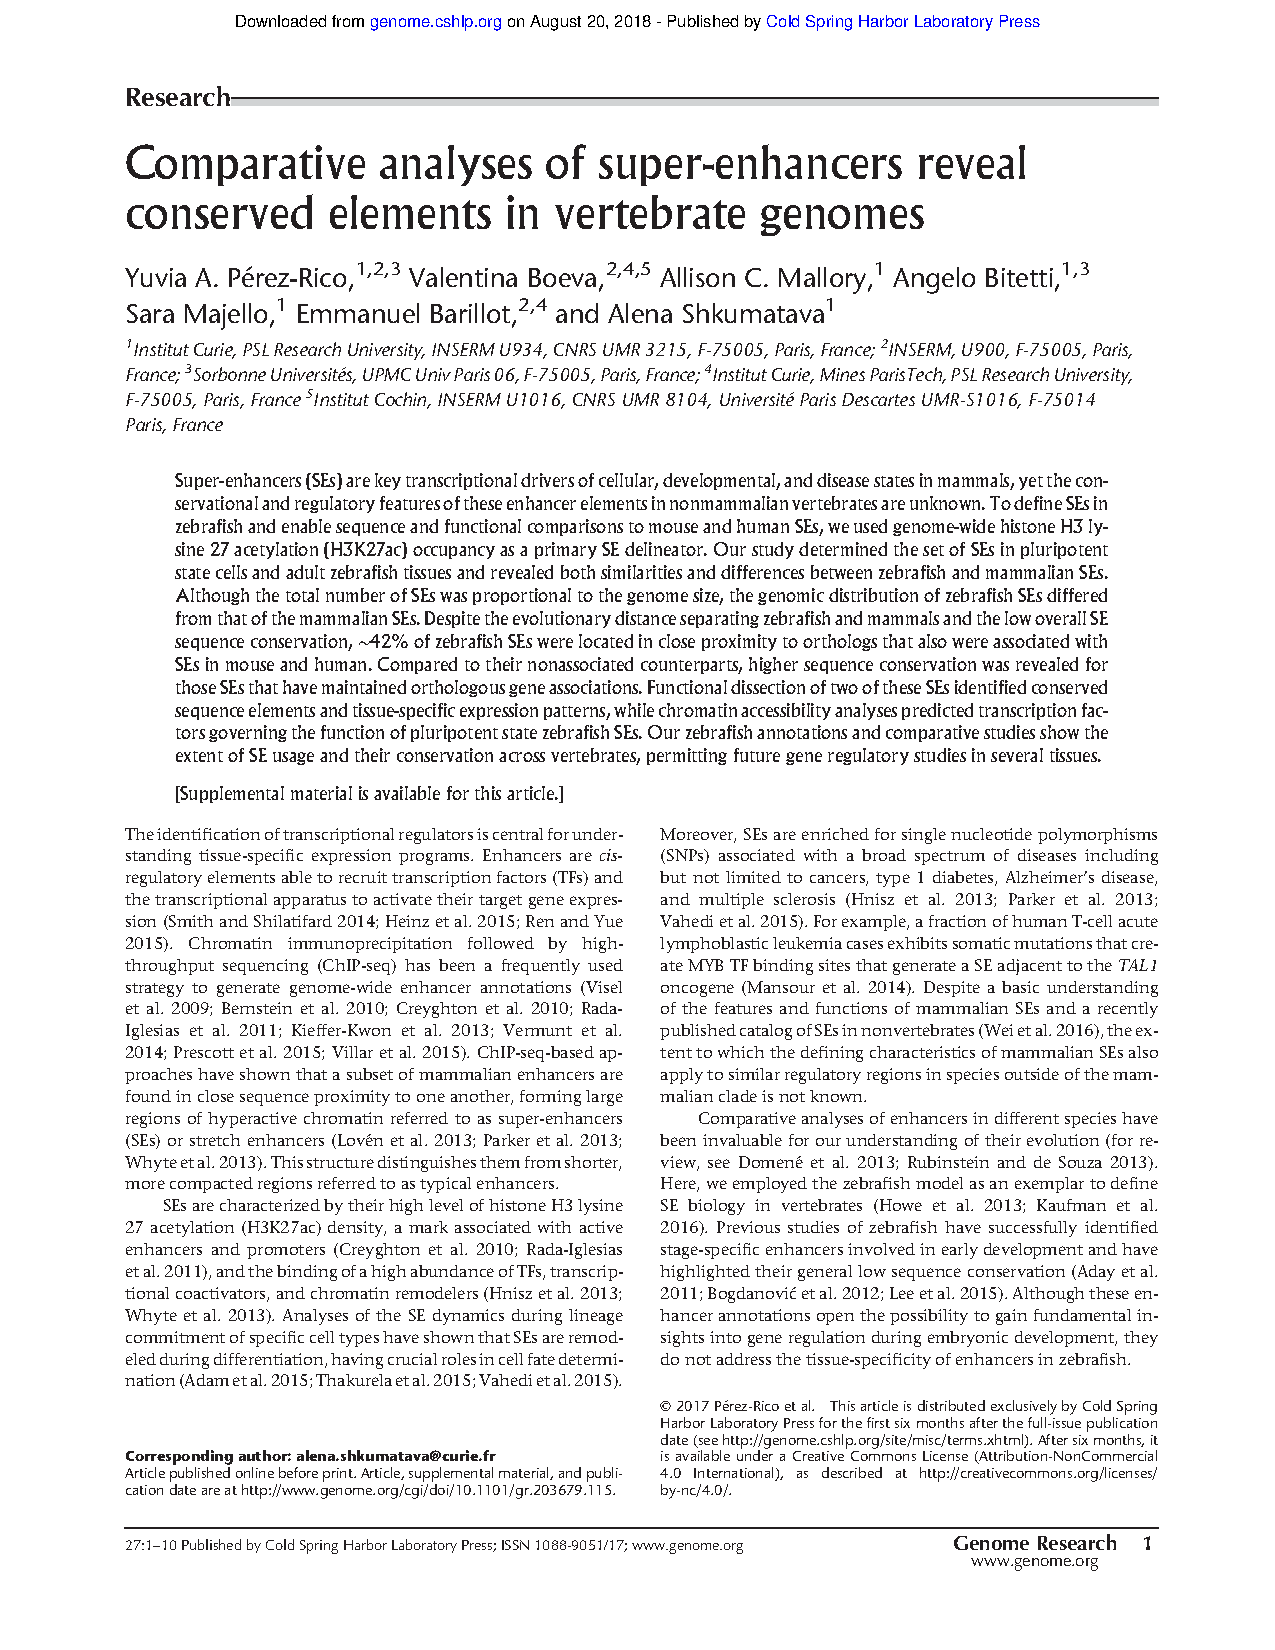
\includepdf[pages=-, pagecommand={\thispagestyle{plain}}, scale=0.95]{GenomeRes_2017/Genome_Res_2017.pdf}

		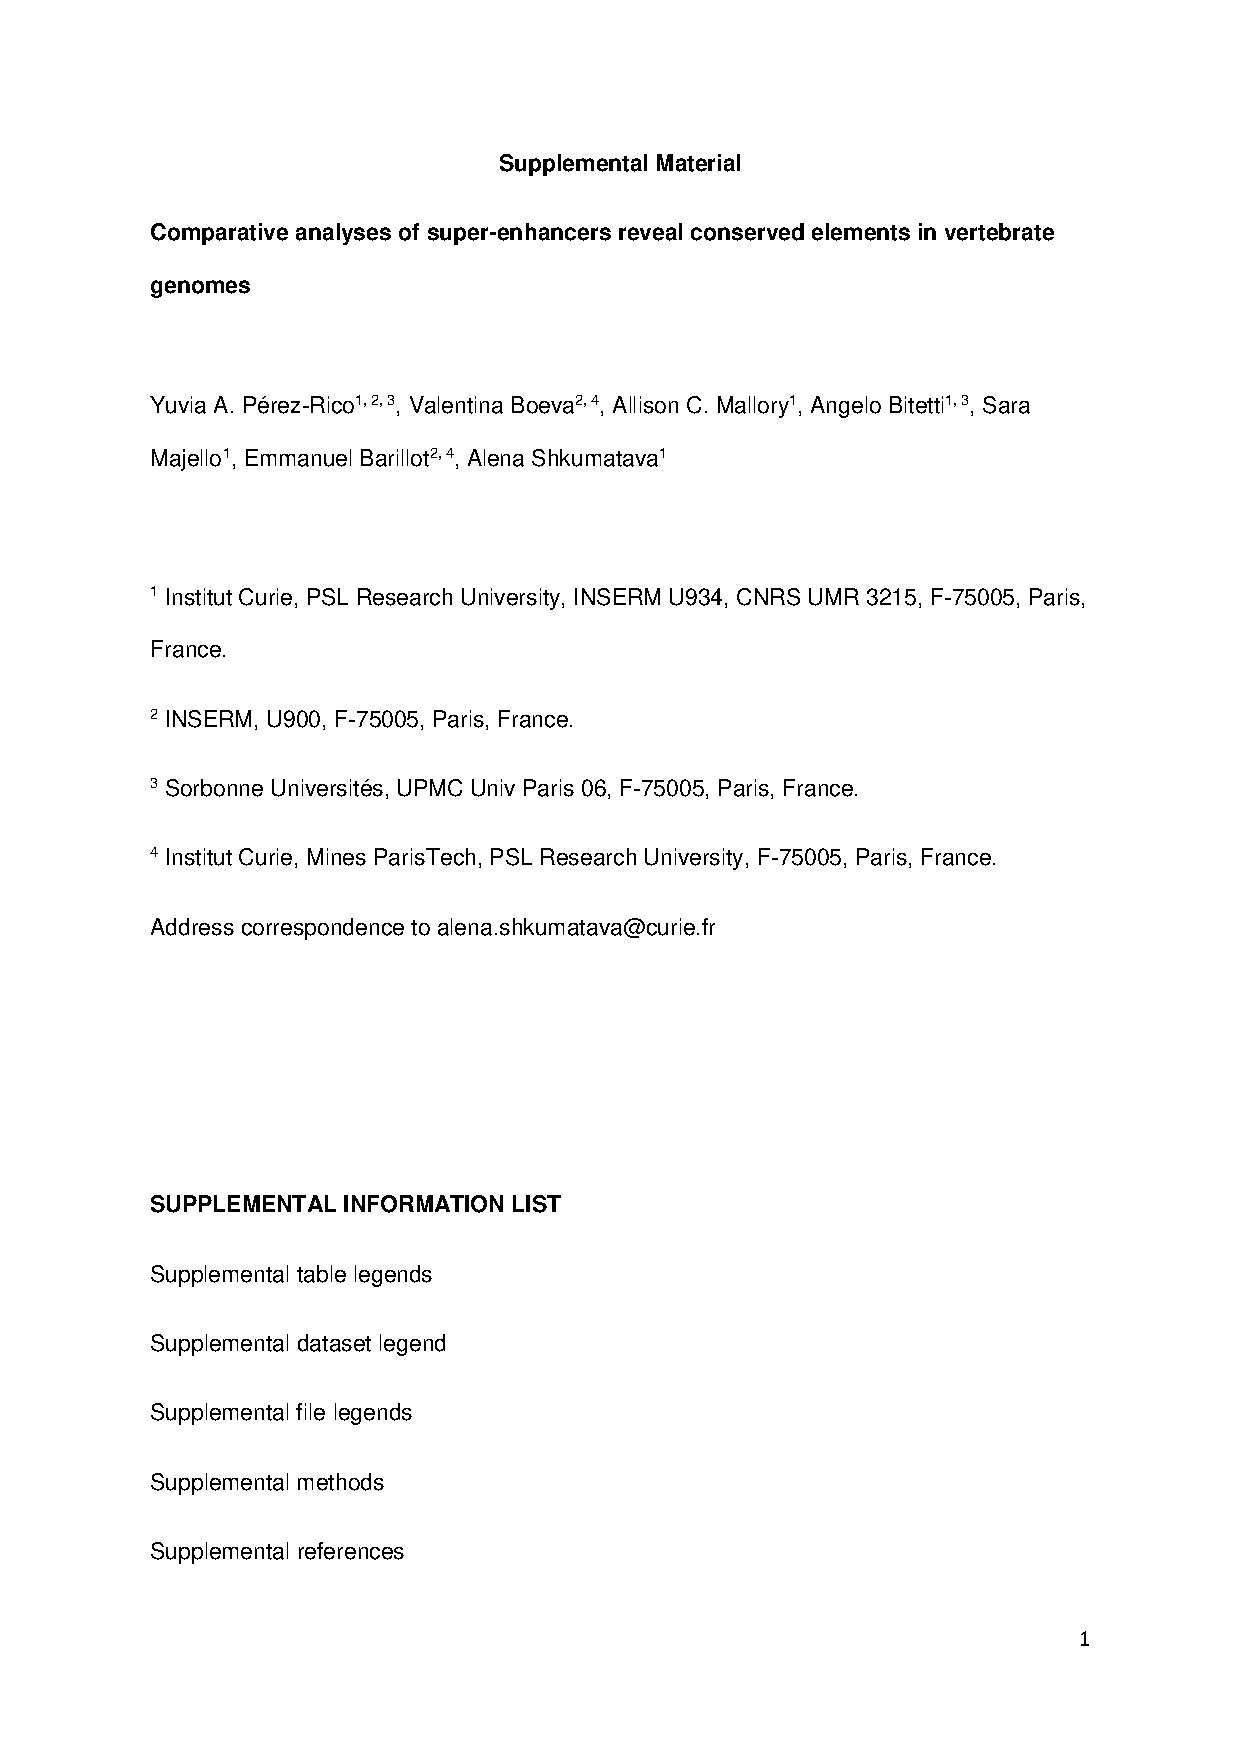
\includepdf[pages=-, pagecommand={\thispagestyle{plain}}, scale=0.9]{GenomeRes_2017/Supplemental_Material.pdf}

		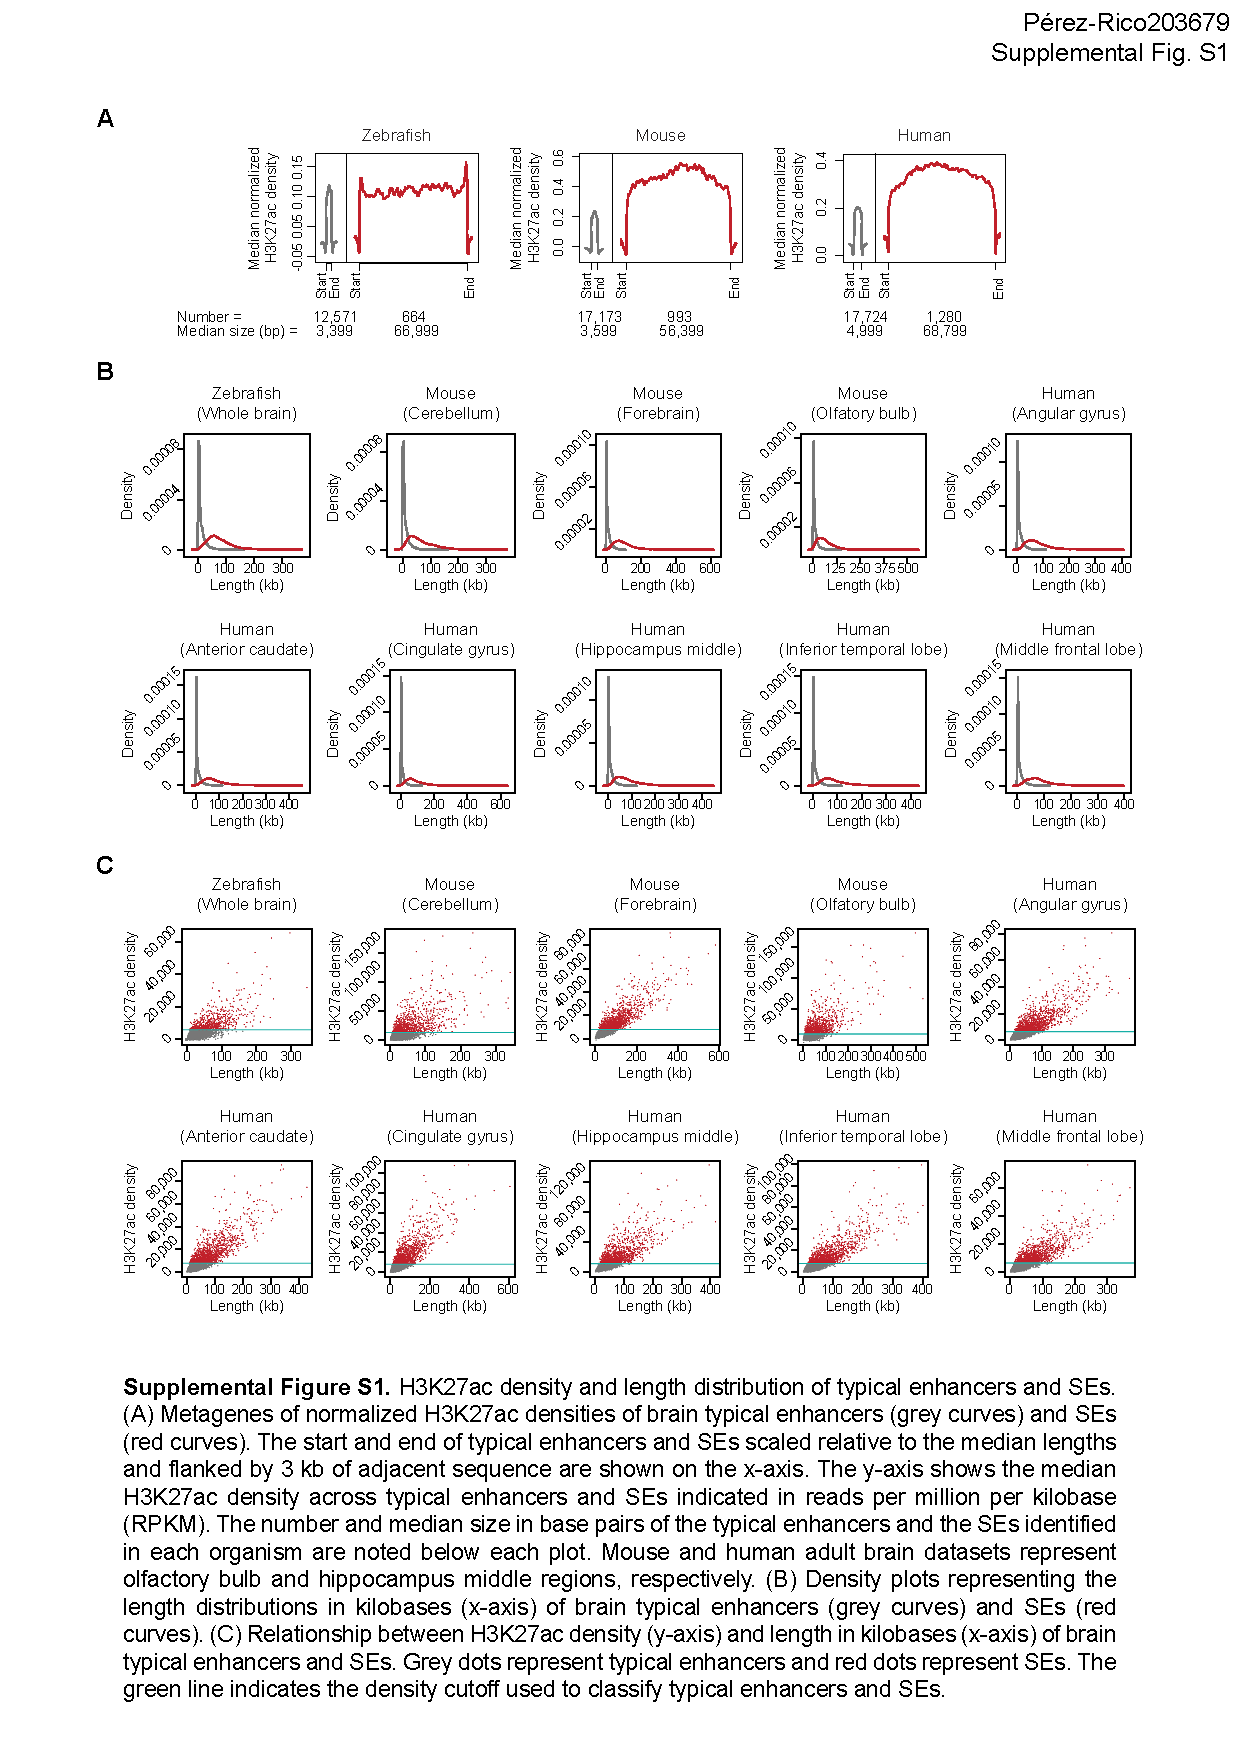
\includepdf[pages=-, pagecommand={\thispagestyle{plain}}, scale=0.8]{GenomeRes_2017/Supplemental_Fig_S1.pdf}

		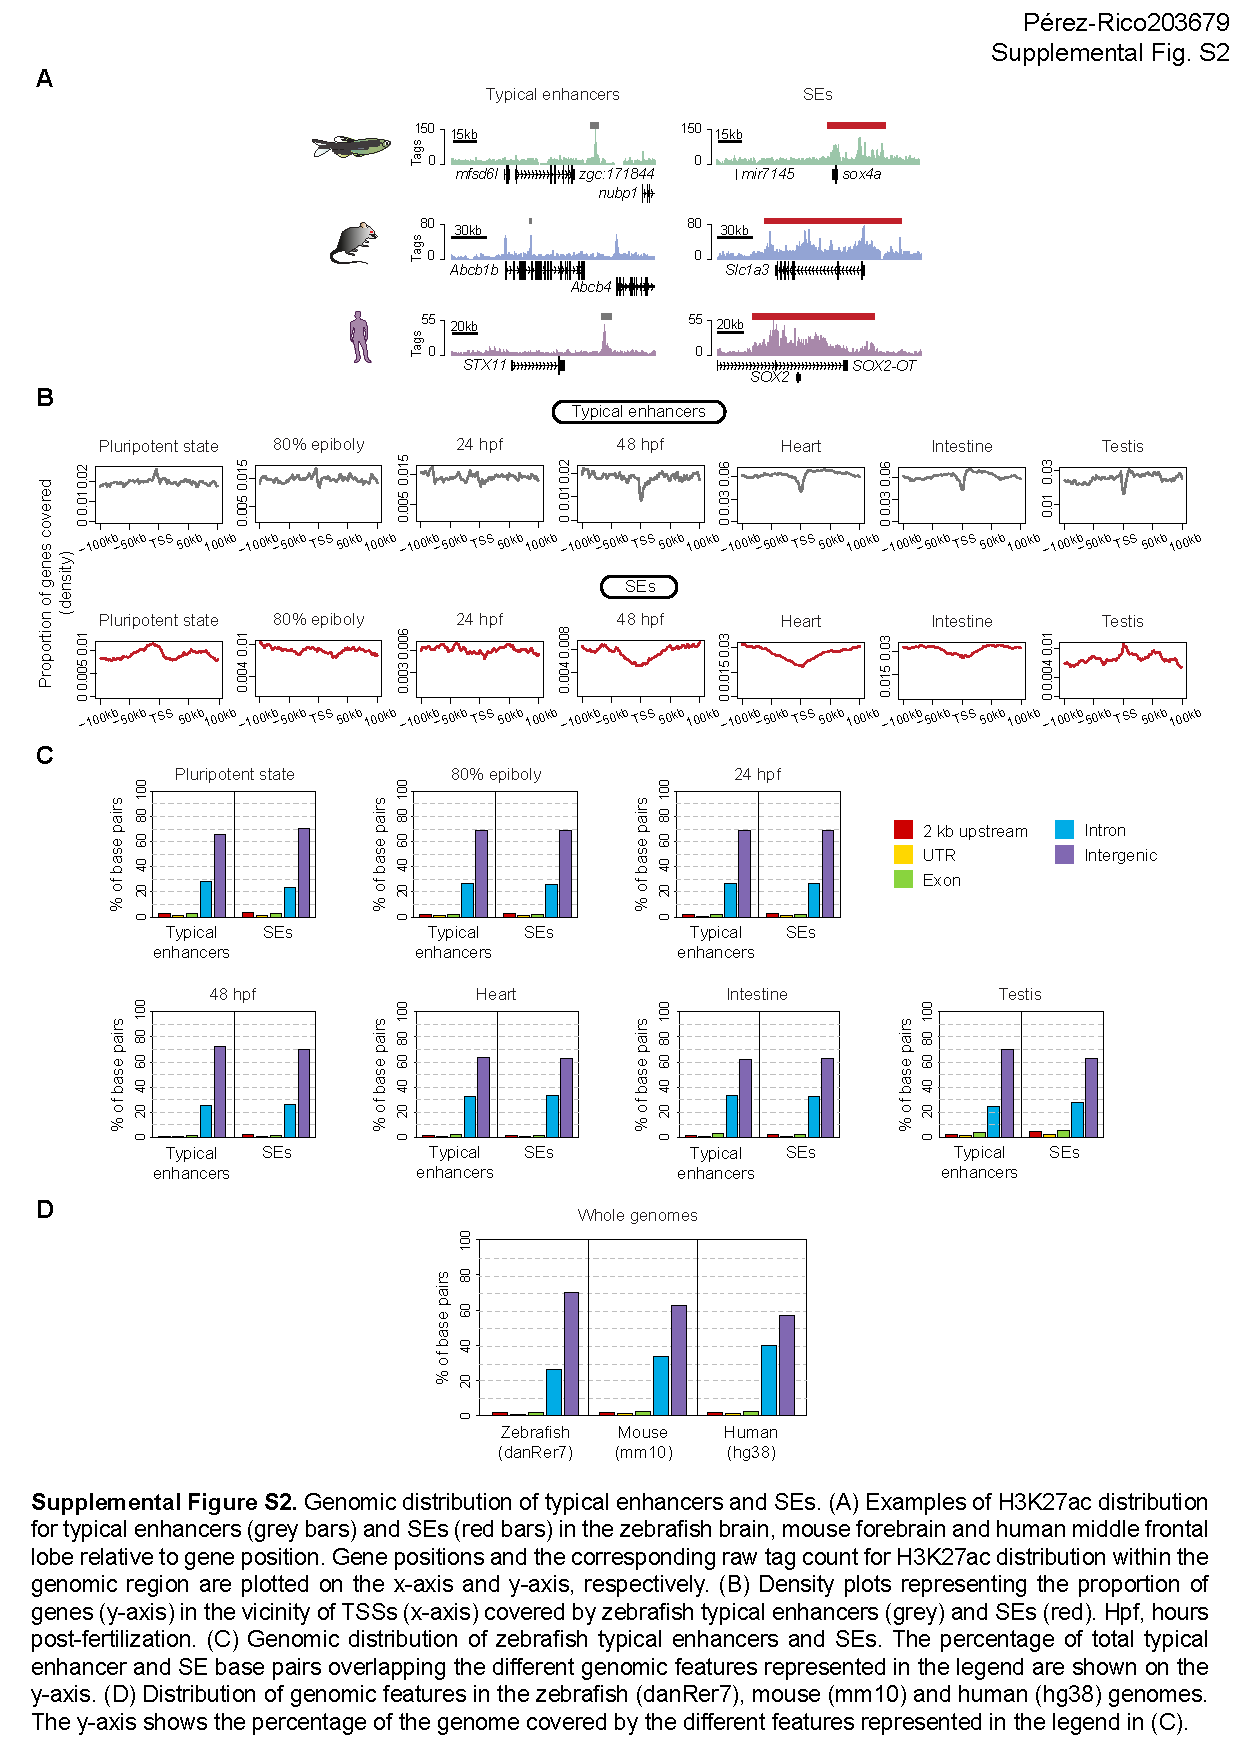
\includepdf[pages=-, pagecommand={\thispagestyle{plain}}, scale=0.8]{GenomeRes_2017/Supplemental_Fig_S2.pdf}

		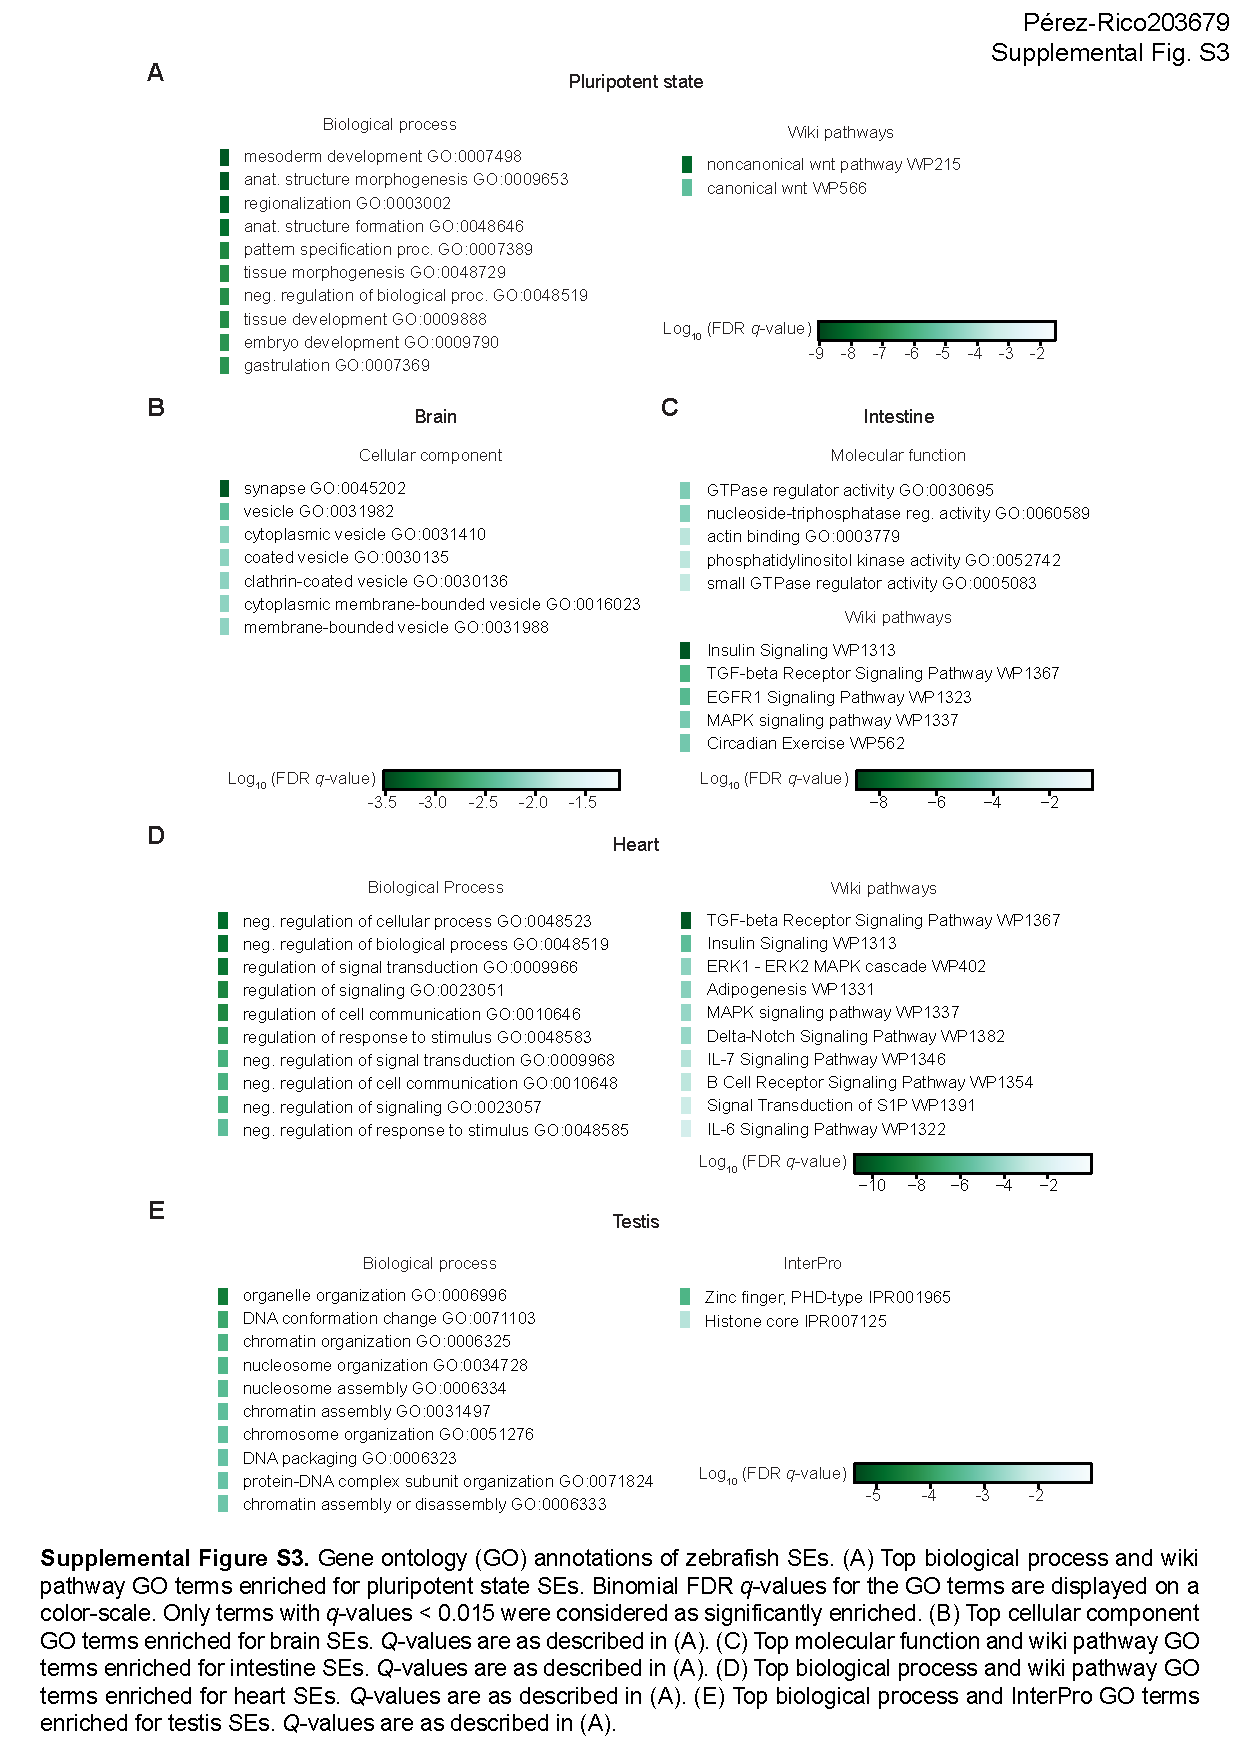
\includepdf[pages=-, pagecommand={\thispagestyle{plain}}, scale=0.8]{GenomeRes_2017/Supplemental_Fig_S3.pdf}

		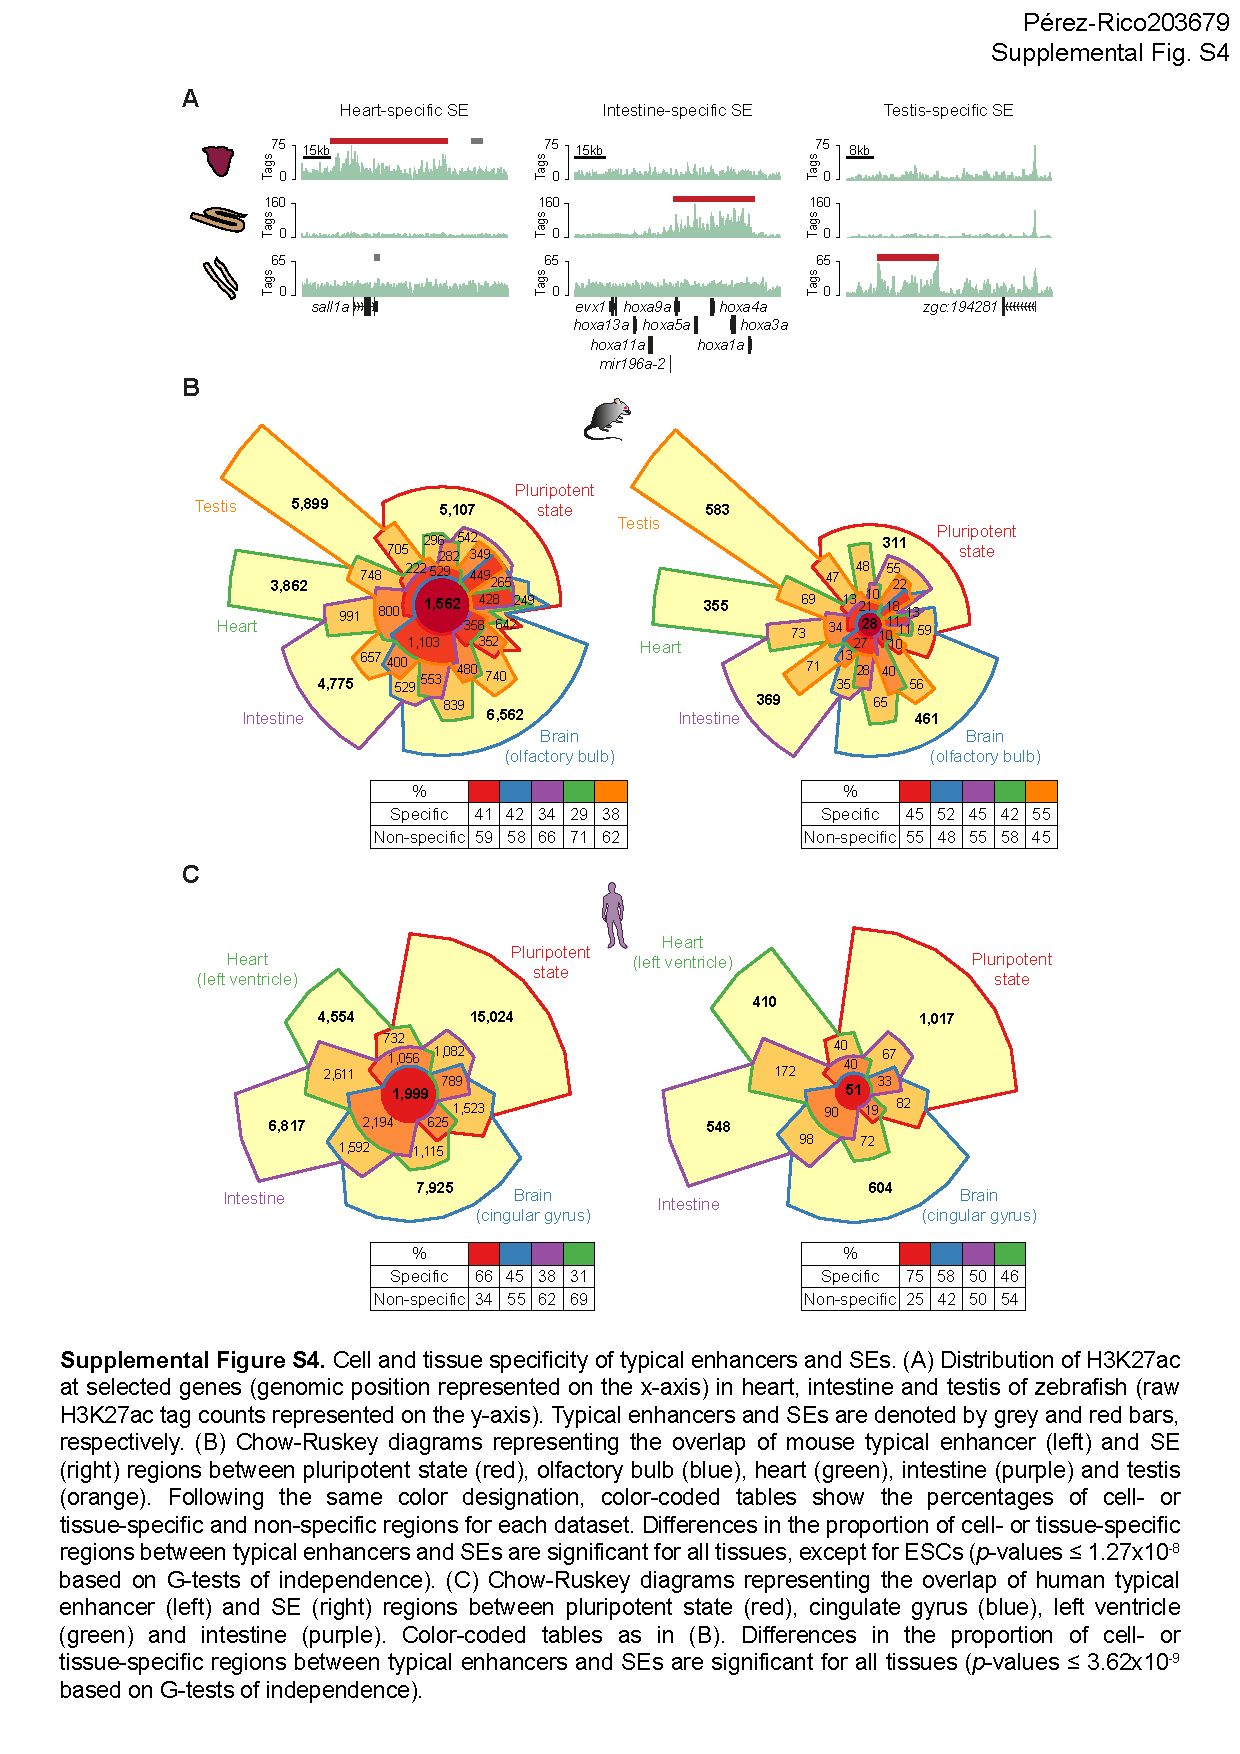
\includepdf[pages=-, pagecommand={\thispagestyle{plain}}, scale=0.8]{GenomeRes_2017/Supplemental_Fig_S4.pdf}

		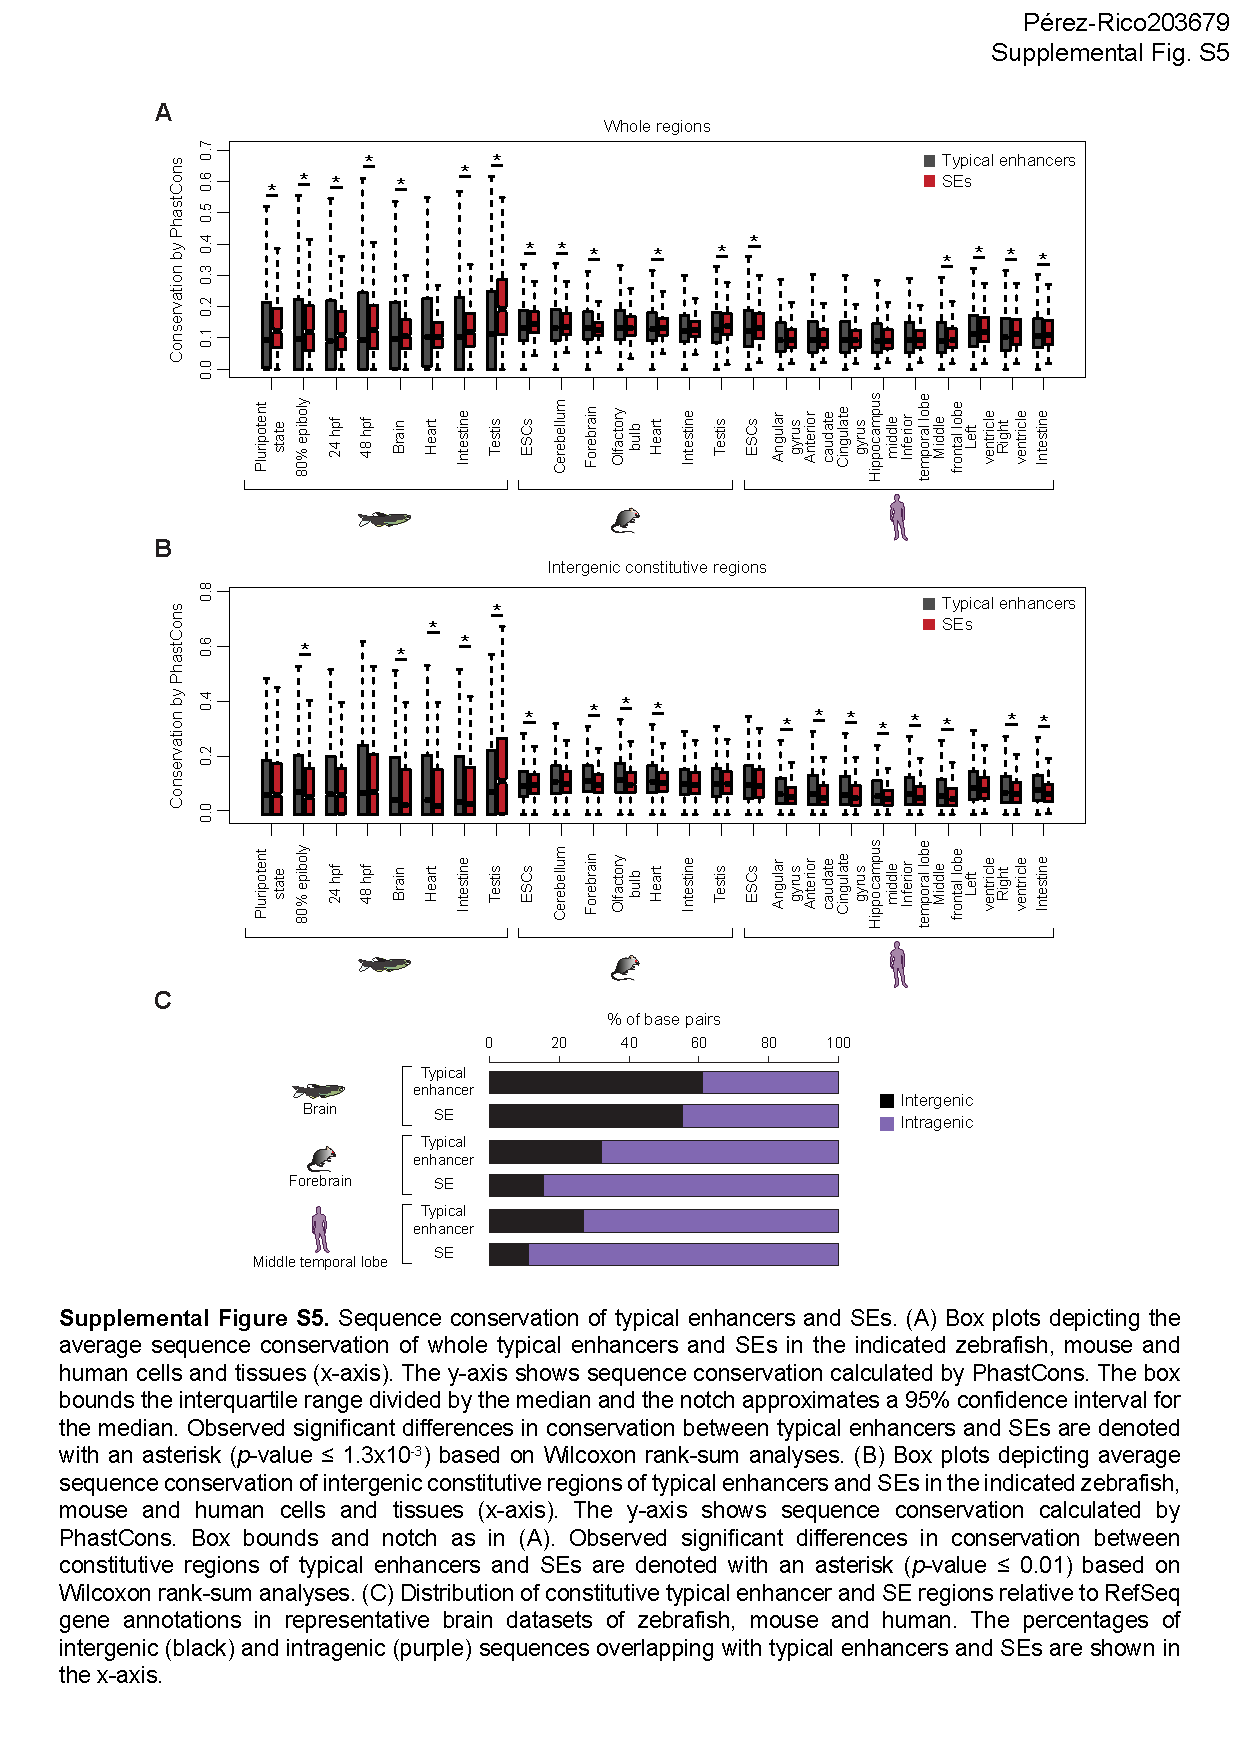
\includepdf[pages=-, pagecommand={\thispagestyle{plain}}, scale=0.8]{GenomeRes_2017/Supplemental_Fig_S5.pdf}

		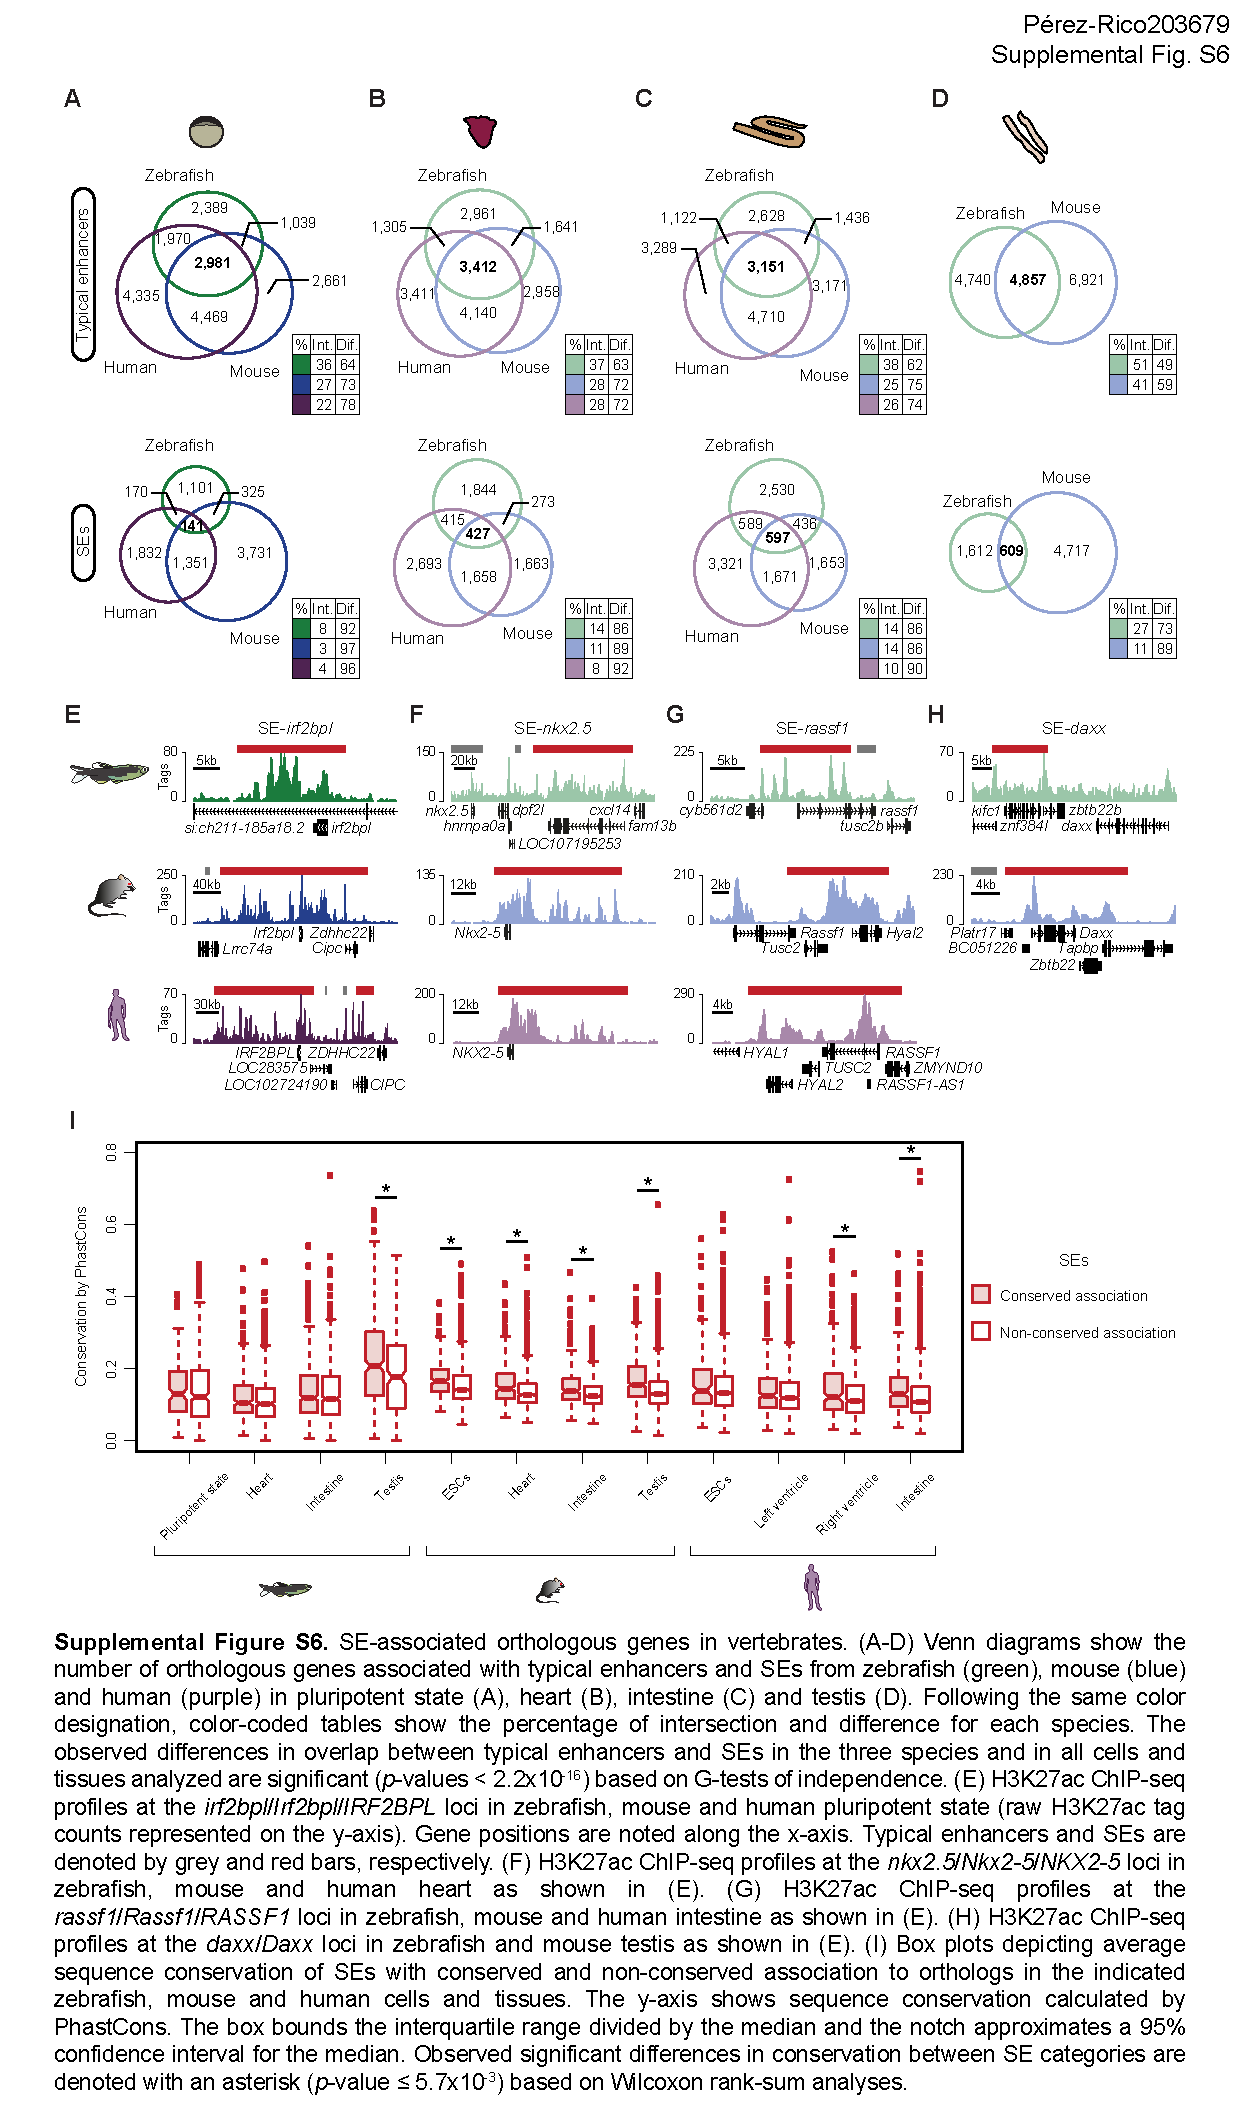
\includepdf[pages=-, pagecommand={\thispagestyle{plain}}, scale=0.8]{GenomeRes_2017/Supplemental_Fig_S6.pdf}

		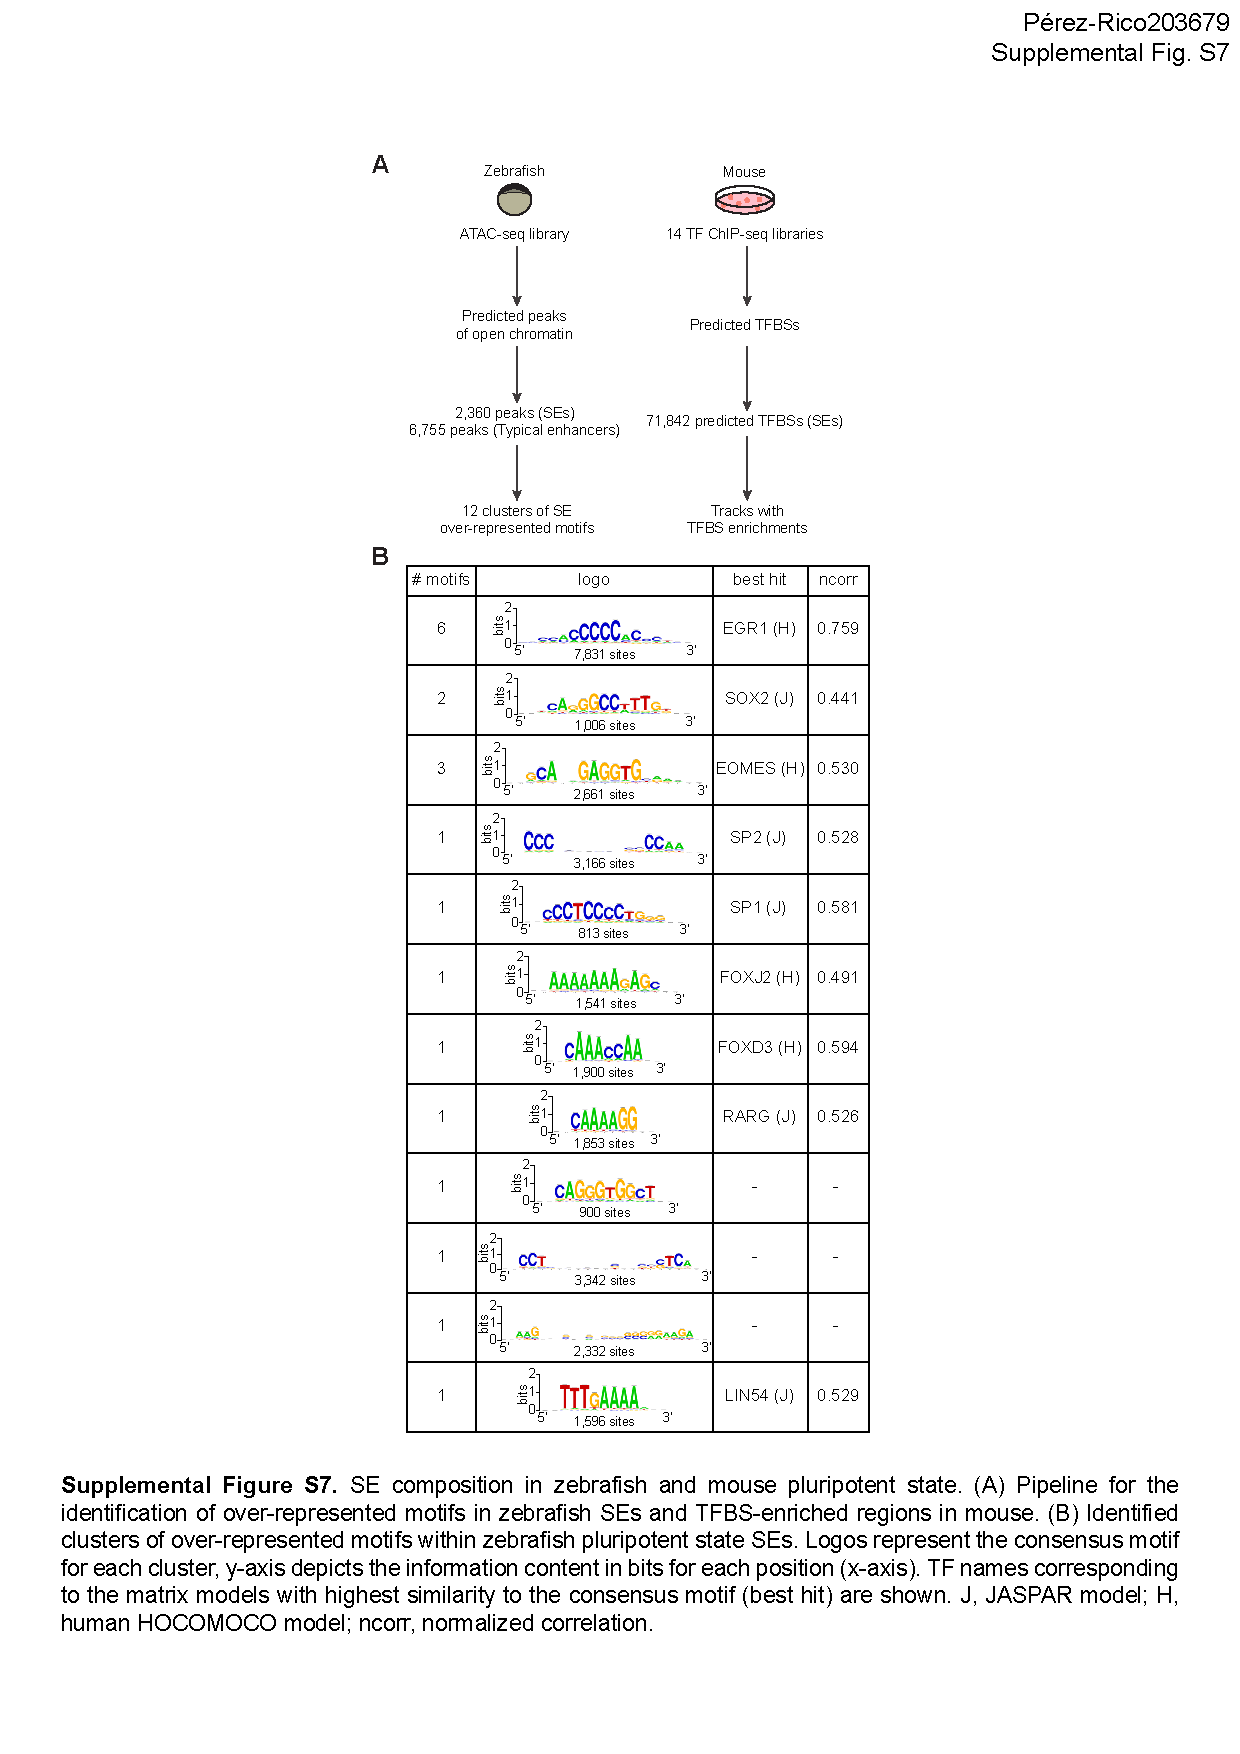
\includepdf[pages=-, pagecommand={\thispagestyle{plain}}, scale=0.8]{GenomeRes_2017/Supplemental_Fig_S7.pdf}

		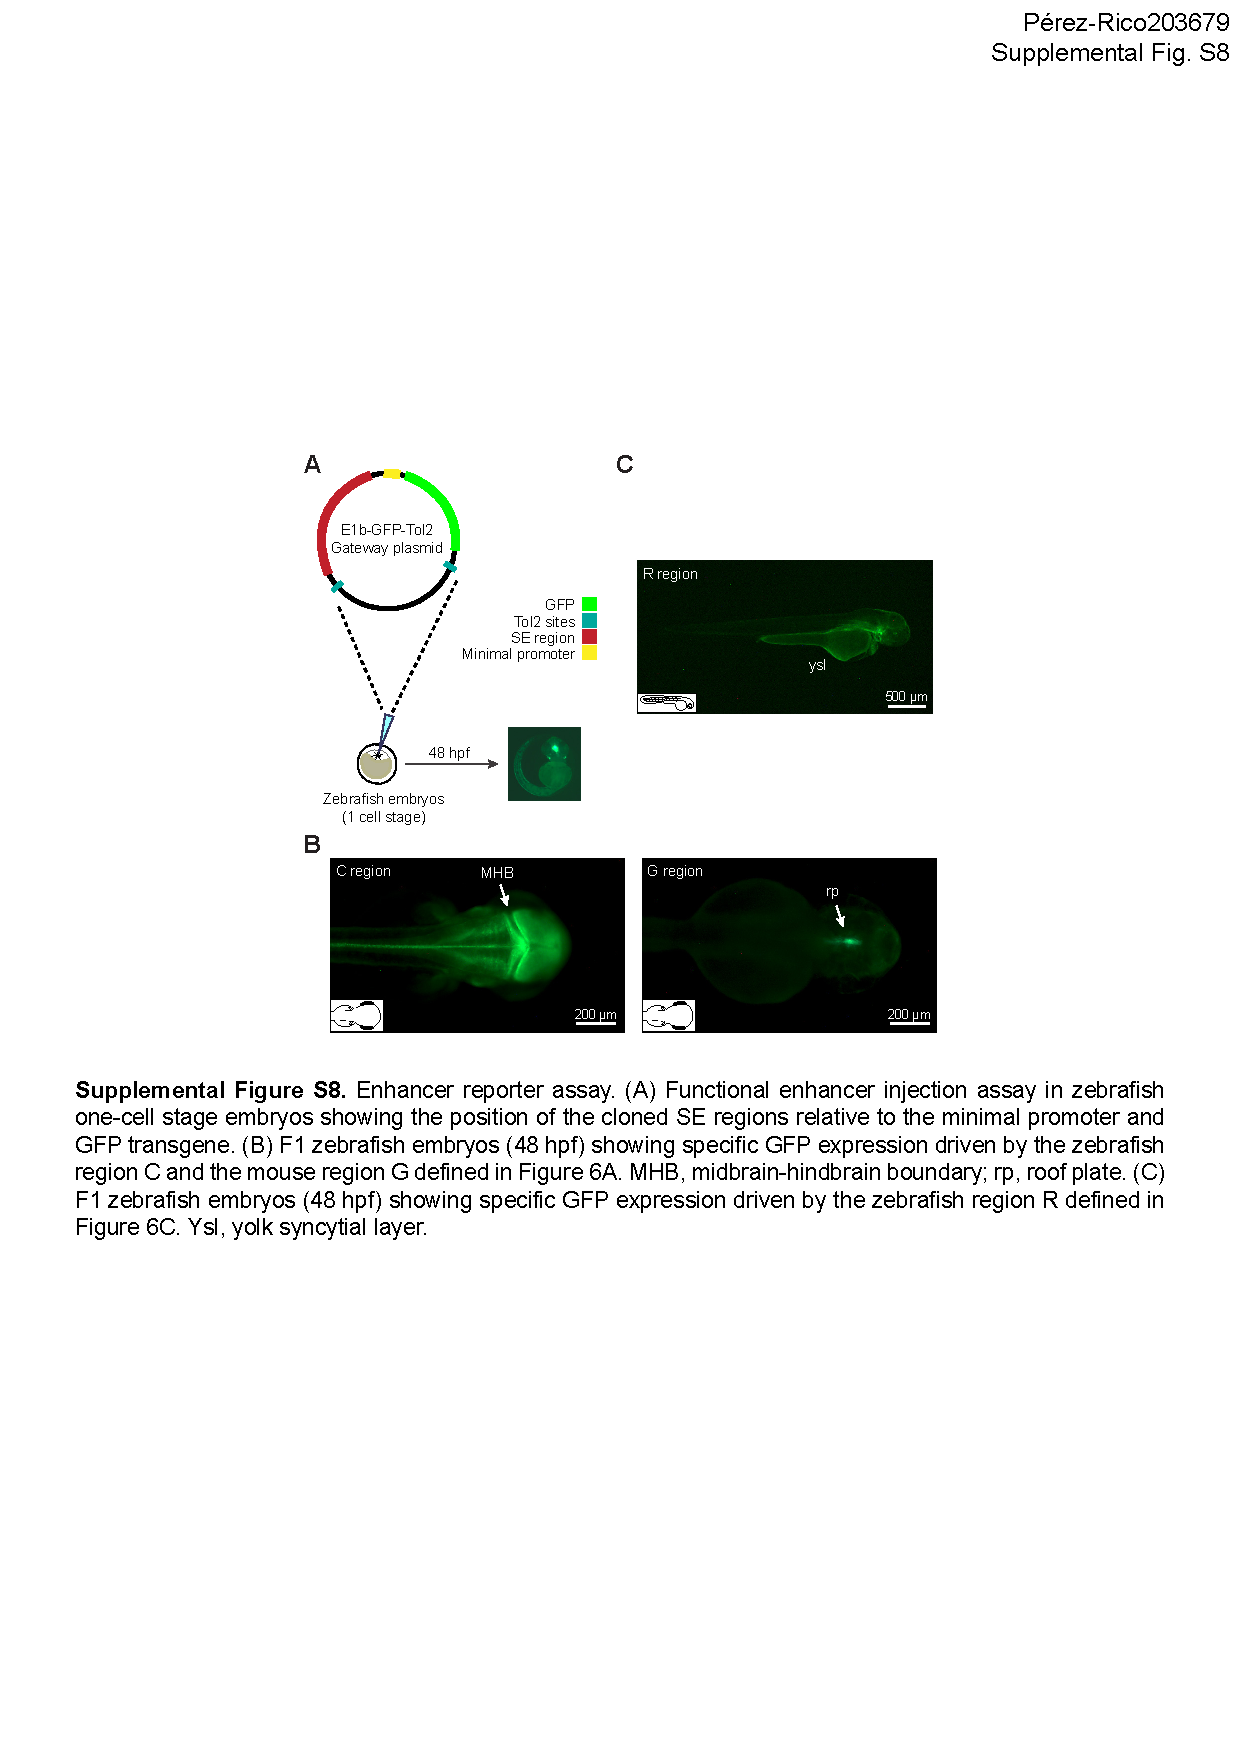
\includepdf[pages=-, pagecommand={\thispagestyle{plain}}, scale=0.8]{GenomeRes_2017/Supplemental_Fig_S8.pdf}

	\section{\textit{In vivo} analysis of CTCF functions in the zebrafish genome}

		The architectural protein CTCF has emerged as a main regulator of the 3D genome organization in mammals. However, the functions of CTCF have been evaluated in a limited number of bilaterian organisms and studies in \textit{Drosophila} have indicated the different roles of CTCF in the genome organization of flies and mammals. Hence, to contribute to the determination of CTCF functions in a phylogenetically distant vertebrate from mammals, genome-wide binding of CTCF has been evaluated for the first time in zebrafish. By integrating additional public genomic data two of the functions of CTCF have been examined.\\ 

		\subsection{Main findings}

			CTCF binding to the zebrafish genome has been difficult to assess, due to the lack of ChIP-seq grade quality antibodies. To overcome this caveat, the CRISPR/Cas9 technology was used to insert an HA-tag in-frame with the coding sequence of \textit{ctcf}. Using this transgenic fish line two biological replicates of CTCF ChIP-seq were generated. ChIP-seq replicates show high correlation and the identified peaks have higher sequence conservation than randomly distributed controls.\\

			Analysis of histone marks over the CTCF peaks show a general enrichment on marks associated with promoters and enhancers. Similarly to described binding sites of CTCF in other vertebrates, extensive motifs of CTCF binding can be identified in a fraction of the CTCF peaks. In addition, repeats enriched on CTCF binding sites were determined, suggesting which sequences could be contributing in the expansion of CTCF sites in this species.\\

			Most of the CTCF peaks localize at intronic and intergenic regions, but there is a small fraction of them that overlaps promoters. For those peaks located in promoter regions, a positive association between the abundance of CTCF and gene expression was identified. Analysis of DNA accessibility supports a mechanism in which CTCF facilitates the establishment of nucleosome free regions in promoters that results in high levels of expression.\\

			Finally, to assess the role of CTCF in the genome organization in zebrafish, Hi-C maps were analyzed. Only a small percentage of CTCF sites is located at contact domain boundaries and, in contrast to its distribution in mammals, CTCF is not enriched at contact domain boundaries of zebrafish embryos. Conversely, marks associated with active transcription show enrichment at boundaries.\\

			In conclusion, the results here presented support the hypothesis of the CTCF code and suggest differences in the relevance of CTCF in the regulation of genome organization in vertebrates. The establishment of this transgenic line opens the possibility to study in more depth the functions of CTCF in zebrafish and therefore, to evaluate its functions in less heterogenic samples.\\


		\includepdf[pages=-, pagecommand={\thispagestyle{plain}}, scale=0.95]{CTCF_paper/Manuscript_CTCF_embryo_analyses_FINAL_THESIS.pdf}

		\setcounter{figure}{0}

		\begin{figure}[h!]
			\centering
			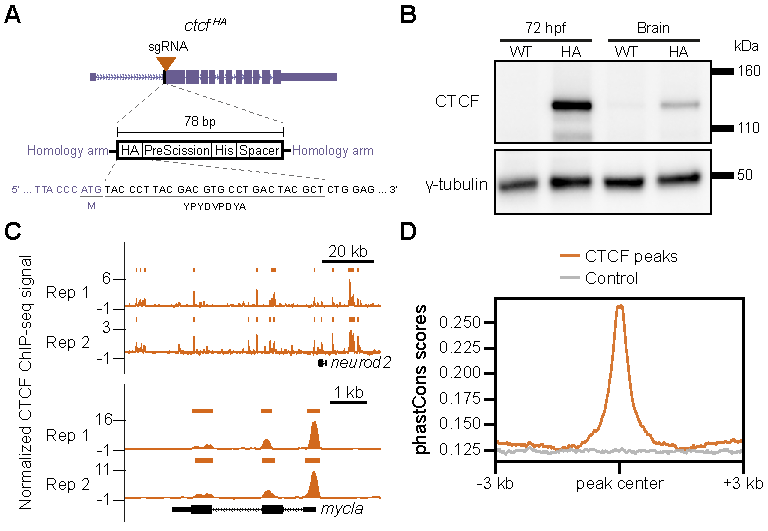
\includegraphics{CTCF_paper/Figure_1.pdf}
  			\caption[one]{Identification of CTCF binding in zebrafish.
(A) Scheme of the \textit{ctcf\textsuperscript{HA}} locus showing the insert used for tagging and the sgRNA site. Sequences at the bottom represent the partial ssDNA oligo corresponding to the HA-tag plus flanking nucleotides and the HA-tag peptide. Sequence in bold is part of the coding sequence; ATG, start codon.
(B) Western blot analysis of wild type (WT) and \textit{ctcf\textsuperscript{HA/HA}} (HA) embryos and adult brains showing specific detection of HA-CTCF in the transgenic line. Molecular weights are indicated on the right.
(C) Tracks showing examples of CTCF peaks in two genomic locations. Displayed signal distributions and peaks correspond to biological replicates (Rep 1, Rep2). Signal is represented on the \textit{y}-axis as -$\log_{10}$ (p-value) of the CTCF ChIP-seq signal.
(D) Distribution of the average sequence conservation of CTCF peaks and control regions using as reference point peak centers.}
			\label{one}
		\end{figure}

		\newpage

		\begin{figure}[h!]
			\centering
			\includegraphics{CTCF_paper/Figure_2.pdf}
  			\caption[two]{Characterization of CTCF peaks and binding sites.
(A) Heat map profiles of four histone marks and ATAC-seq data at CTCF peaks ranked by decreasing CTCF ChIP-seq signal over the displayed region. Normalized signal is shown in FPM (fragments per million mapped fragments) for ATAC-seq and in RPKM (reads per kilobase million) for histone marks.
(B) Dendogram representing the hierarchical clustering results of CTCF and CTCFL motifs. Ncor, normalized Pearson correlation.
(C) Top, histogram showing the number of co-occurrences of the CTCF core and upstream motif at different spacing distances (6 – 25 bp). Non-significant enriched spacings are colored in grey, and enrichments are shown in pink, whereas the highest enrichments are shown in red. Bottom, inferred upstream motifs using the sequences matching to the reference motif at the indicated distances from the CTCF core motif.
(D) Proportion of the top five DNA transposon types enriched on CTCF binding sites. For control regions the mean and the standard deviation (error bars) calculated by bootstrap analyses are shown.}
			\label{two}
		\end{figure}

		\newpage

		\begin{figure}[h!]
			\centering
			\includegraphics{CTCF_paper/Figure_3.pdf}
  			\caption[three]{High CTCF binding at promoters associates with high expression levels.
(A) Distribution of CTCF peaks in different categories of genomic regions. Percentages correspond to the percentage of CTCF peaks in chromosomes for each category.
(B) Average CTCF ChIP-seq signal profiles over the TSS region of genes stratified based on the score of CTCF peaks on their promoters (Low, Medium, High) and genes with no CTCF peaks (No peak).
(C) Contingency tables showing the number of gene promoters for each of the three defined categories (color-coded as in B) that contain a CTCF motif irrespectively of its orientation (top) and in the same orientation than transcription (bottom).
(D) Expression of the stratified gene categories and genes without CTCF peaks at promoters. Observed differences in the distributions are denoted as significant (*) and non-significant (n.s.) according to two-sided Wilcoxon rank-sum test ($p-value \le 1.5x10-5$).
(E) Average ATAC-seq signal profiles over the TSS region of genes stratified based on the score of CTCF peaks on their promoters.
(F-I) Average ChIP-seq signal profiles of (F) H3K4me1, (G) H3K4me3, (H) H3K27ac and (I) H3K36me3 over gene bodies and flanking sequence of the three categories of genes with CTCF bound at promoters.}
			\label{three}
		\end{figure}

		\newpage

		\begin{figure}[h!]
			\centering
			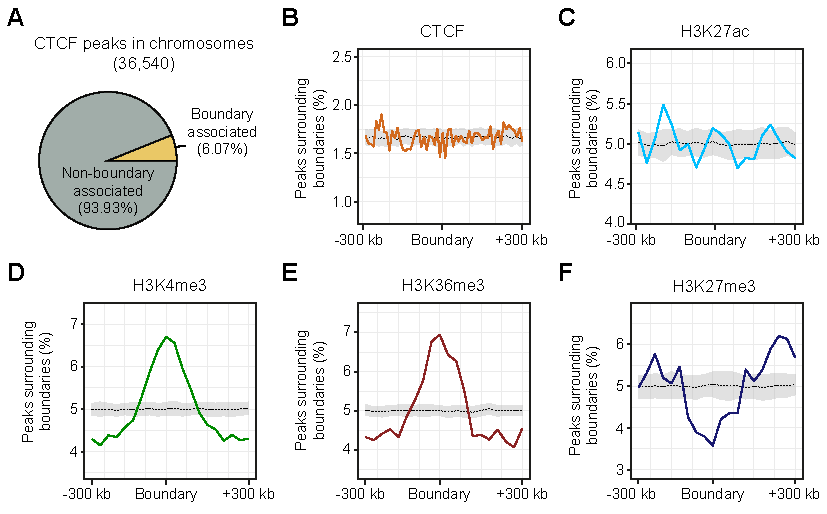
\includegraphics{CTCF_paper/Figure_4.pdf}
  			\caption[three]{Active chromatin marks, but no CTCF, are enriched at domain boundaries.
(A) Classification of CTCF peaks in chromosomes relative to contact domain boundaries.
(B) Distribution of CTCF peaks (orange) along 600 kb regions centered on contact domain boundaries (\textit{x}-axis). The \textit{y}-axis shows the percentage of total peak counts in the 600 kb region located at each genomic position. The dash line represents the mean background distribution and the grey ribbon depicts the $\pm$ 1 standard deviation range from the mean.
(C-F) Distribution of significant (C) H3K27ac, (D) H3K4me3, (E) H3K36me3 and (F) H3K27me3 peaks along contact boundary regions as described for B.}
			\label{four}
		\end{figure}


		\newpage

		\renewcommand{\figurename}{Supplemental Figure}
		\setcounter{figure}{0}

		\begin{figure}[h!]
			\centering
			\includegraphics[width=14cm,height=12cm]{CTCF_paper/Figure_S1.pdf}
  			\caption[five]{Characterization of the \textit{ctcf\textsuperscript{HA}} line.
(A) Images of wild type (WT) and \textit{ctcf\textsuperscript{HA/HA}} embryos during early development. Scale bars for each stage are displayed. Hfp, hours post-fertilization.
(B) Images of wild type (WT) and \textit{ctcf\textsuperscript{HA/HA}} adult fish. Representative fish of each sex and genotype are shown. Scale bars for each genotype are displayed.
(C) Whole gel of the Western blot shown on Fig. 1B and performed using wild type (WT) and \textit{ctcf\textsuperscript{HA/HA}} (HA) embryos and adult brains. Molecular weights are indicated on the left.}
			\label{five}
		\end{figure}

		\newpage

		\begin{figure}[h!]
			\centering
			\includegraphics[width=14cm,height=14cm]{CTCF_paper/Figure_S2.pdf}
  			\caption[six]{Identification of CTCF binding in zebrafish.
(A) Circos plot showing the average CTCF ChIP-seq signal of the two biological replicates in all chromosomes binned in 1 Mb windows. The CTCF peak enrichment track represents enrichment of CTCF peaks identified with combined replicates in 1 Mb windows. Zoom-in of chromosome 15 is displayed.
(B) Correlation between CTCF ChIP-seq biological replicates. In the scatter plot each dot represents one 1Mb bin and the axes correspond to the average signals in replicate 1 (\textit{y}-axis) and replicate 2 (\textit{x}-axis).
(C) Genome track showing the distributions of CTCF signal of biological replicates at the \textit{ctcf} locus.
(D) Distribution of the average sequence conservation of non-exonic CTCF peaks and control regions using as reference point the center of peaks and controls.}
			\label{six}
		\end{figure}

		\newpage

		\begin{figure}[h!]
			\centering
			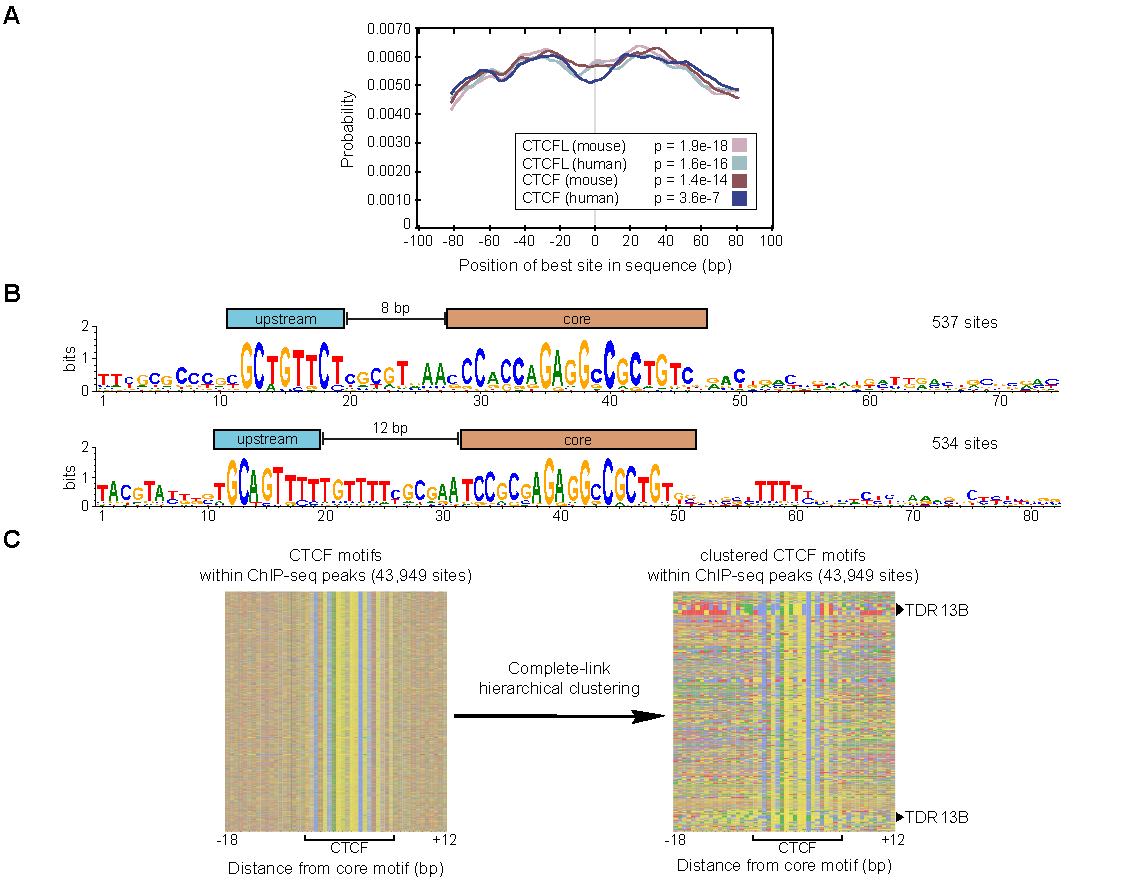
\includegraphics[width=14cm,height=13cm]{CTCF_paper/Figure_S3.pdf}
  			\caption[seven]{Analysis of CTCF binding sites.
(A) Probability distribution of the best motif matches per CTCF peak sequence calculated for the four indicated motifs. P-values support the central enrichment of the motifs.
(B) Extended motif logos for the sequences containing matches to the CTCF core and upstream motifs at spacing distances of 8 (top) and 12 bp (bottom). The number of sequences used to generate the logos is shown.
(C)  Left, color chart representing all the sequences with CTCF sites centered on the region matching to the zebrafish CTCF motif. Right, color chart with the same sequences clustered by edit distances. Clustered sequences indicating the enrichment on TDR13B repeats are indicated with triangles. Nucleotides are represented as follows: A = green, T = red, C = blue, G = yellow.}
			\label{seven}
		\end{figure}

		\newpage

		\begin{figure}[h!]
			\centering
			\includegraphics[width=14cm,height=16cm]{CTCF_paper/Figure_S4.pdf}
  			\caption[eight]{Analysis of promoters with and without CTCF peaks.
(A) Profiles and heat maps of ATAC-seq signal in promoters that do not contain a CTCF peak. Promoters were assigned to eight clusters using k-means.
(B) Genome browser showing strand-specific RNA-seq, CTCF ChIP-seq, ATAC-seq and histone ChIP-seq signal around the \textit{pbx4} gene, which promoter has a highly-bound CTCF peak.
(C) Average H3K27me3 ChIP-seq signal profiles over gene bodies and flanking sequence of the three categories of genes with CTCF bound at promoters.
(D) Average H3K27me3 ChIP-seq signal profiles over gene bodies and flanking sequence of genes without CTCF peaks at promoters.
(E) Contingency table of promoters showing their classification based on the presence/absence of CTCF peaks and their bivalency status. The top pie chart represents all promoters classified based on bivalency status. Pie charts at the bottom represent bivalent promoters (left) and non-bivalent promoters (right) with or without CTCF peaks.}
			\label{eight}
		\end{figure}

		\newpage

		\begin{figure}[h!]
			\centering
			\includegraphics[width=14cm,height=17cm]{CTCF_paper/Figure_S5.pdf}
  			\caption[nine]{Visualization of Hi-C maps of zebrafish embryos shows Rabl configuration of chromosomes.
(A-B) Hi-C maps of zebrafish at (A) 24 hpf and (B) 4 hpf showing intra-chromosomal and inter-chromosomal interaction signal for all 25 chromosomes. Arrowheads point to representative enrichments of interaction between centromeres and telomeres.
(C) Karyotype of the zebrafish chromosomes showing the locations of the intersections between the two strong diagonals visualized on the Hi-C maps (red) and centromeres (blue).
(D) Distribution of CTCF motifs (orange) along 600 kb regions centered on contact domain boundaries (\textit{x}-axis). The \textit{y}-axis shows the percentage of total peak counts in the 600 kb region located at each genomic position. The dash line represents the mean background distribution and the grey ribbon depicts the $\pm$ 1 standard deviation range from the mean.}
			\label{nine}
		\end{figure}

		\newpage

		\includepdf[pages=-, pagecommand={\thispagestyle{plain}}, scale=0.8]{CTCF_paper/Supplemental_File_S1.pdf}

		\includepdf[pages=-, pagecommand={\thispagestyle{plain}}, scale=0.8]{CTCF_paper/Supplemental_Table_S1.pdf}

		\includepdf[pages=-, pagecommand={\thispagestyle{plain}}, scale=0.8]{CTCF_paper/Supplemental_Table_S2.pdf}




	\chapter{Discussion and perspectives}

Extensive analyses of super-enhancers and CTCF in mammalian genomes indicate that these two regulators have major roles in the 3D genome organization, however, little is known about their functions in other vertebrates. In this work, I present the first steps towards the elucidation of super-enhancer and CTCF functions in the zebrafish genome. The results confirm that super-enhancers in zebrafish are cell- and tissue-specific, indicating an association with the establishment of cell identity, and highlight the benefits of analyzing whole super-enhancer regions instead of limiting the analysis to single enhancers. Regarding the analyses of CTCF binding in the zebrafish genome, the results support the notion of a CTCF ``code’’ widespread in vertebrate genomes. Conversely, in spite of the similar genome-wide distribution of CTCF relative to transcription units in zebrafish and mammalian genomes, our results show discrepancy in the distribution of CTCF around contact domains, suggesting differences in the regulation of the 3D genome organization. Future work should aim to analyze the interplay of super-enhancers and CTCF towards the identification of determinants of the genome organization in zebrafish and potential novel regulators.\\

	\section{Comparative analyses of super-enhancers reveal conserved elements in vertebrate genomes}

		\subsection{Zebrafish super-enhancer characteristics}

Out of the previously described characteristics of super-enhancers in mammals, analysis of zebrafish super-enhancers was focused on their cell and tissue specificity and on their distribution relative to gene bodies. Whereas the high cell and tissue specificity of zebrafish super-enhancers was confirmed, differences in their distribution in the genome were observed. Contrary to mouse and human super-enhancers located in the vicinity of genes, zebrafish super-enhancers are not preferentially located downstream of the TSSs and, in general, they are not enriched over gene bodies. If this observation has an impact in the relationship between super-enhancers and their targets genes has not been evaluated. In addition, the identity of the genes with super-enhancer enrichment in mouse and human was not analyzed to assess if those genes show particular features or if they correspond to specific gene classes. Also, the reference annotations of mouse and human are more complete and curated; therefore, the analyses of zebrafish super-enhancers could have been partially hampered by missing gene annotations, including those of noncoding RNA genes.\\

It remains to be tested if other super-enhancer characteristics described in mammals also apply to zebrafish super-enhancers. Among those characteristics, it will be important to determine if zebrafish super-enhancers have high sensitivity to perturbations of their binding proteins (Whyte et al. 2013; Lovén et al. 2013; Vahedi et al. 2015), if they are also confined in insulated neighborhoods (Dowen et al. 2014) and if they have spatial colocalization (Beagrie et al. 2017) to create complex regulatory networks (Novo et al. 2018). These characteristics will be important to analyze because they can provide clues about the establishment of super-enhancers in light of the phase separation and loop extrusion models (Fudenberg et al. 2016; Hnisz et al. 2017). In fact, super-enhancers are involved in intra- and inter-chromosomal interactions in 8 and 24 hpf zebrafish embryos (Kaaij et al. 2018), indicating that super-enhancers in zebrafish might also form phase separated foci.\\

		\subsection{Analysis of super-enhancer sequence conservation}

Sequence conservation assessed by PhastCons scores showed that super-enhancers do not have higher conservation than typical enhancers, and only those super-enhancers that are associated with orthologs in zebrafish, mouse and human show significant higher sequence conservation than the rest of super-enhancers. Nevertheless, it was not analyzed if these increase in sequence conservation was a general increase of conservation in the whole super-enhancer regions, or if it was rather caused by small regions with high conservation values. It is important to analyze this difference, as small intergenic regions of high conservation could be an indicative of conserved \textit{cis}-regulatory modules. Therefore, this information could be used as a basis to identify super-enhancers containing regions driving conserved patterns of expression, similar to the regions described for SE-\textit{zic2a} and SE-\textit{irf2bpl}. Independently of their sequence conservation, the identified subset of super-enhancers with conserved association to orthologous genes could also be used to predict short regions of conserved functionally, as it has been previously performed using noncoding sequence elements with no evident conservation based on pair-wise comparisons of distant genomes (Taher et al. 2011). Notably, the scanning of the identified regions driving similar patterns of gene expression within SE-\textit{zic2a} and SE-\textit{irf2bpl} did not show any specific conserved TFBS grammar, suggesting that specialized algorithms to identify low conserved regulatory modules (Taher et al. 2011) and the scanning with more TF matrix models will be required to identify the mechanism governing their functional conservation. These analyses would have to be complemented with enhancer reporter assays bashing the regions to identify the minimal sequences driving equivalent expression patterns.\\

In addition, the process that leads to establishment of super-enhancers near orthologous genes has not been assessed. One possibility is that these super-enhancers are located in syntenic blocks in the three species, indicating a common origin. This evidence combined with annotations of contact domains can be used to analyze if super-enhancers and those orthologs are located within the same contact domain, explaining why their preferential associations have been maintained in evolution. Another possibility is that these super-enhancers emerged independently in each species, which is also a viable explanation considering that super-enhancers can emerged from single nucleation events (Mansour et al. 2014).\\

		\subsection{Improvement in the annotation of target genes}

Super-enhancer target genes were annotated based on a simple method relying on sequence proximity. Comparison of annotations based on proximity and ChIA-PET data have shown good correlation (Dowen et al. 2014). Nevertheless, it is clear that annotations based on chromosome conformation capture data are more reliable because enhancers can control the expression of target genes that are located more distantly than 100 kb (Sanyal et al. 2012), the proximity value used to annotate target genes. Considering that adjacent super-enhancers and genes could be located in different contact domains it is likely that, besides disregarding true target genes, annotations solely based on proximity potentially include false positive target genes.\\

		\subsection{Identification of TFs governing super-enhancer functions}

Although zebrafish ATAC-seq data was available for the dome stage, the performed enhancer reporter assays and comparison with nanog ChIP-seq data indicate that ATAC-seq is not sufficient to comprehensively identify TFBS epicenters. Therefore, experimental data sets interrogating the binding of more TFs are required to better characterize the TFs enriched at super-enhancers and their cooperativity within them. Despite the lack of antibodies with reactivity to zebrafish, determination of TF binding in the genome can now be achieved using CRISPR/Cas9, as shown for CTCF.\\

Differential analysis of ATAC-seq regions within typical enhancers and super-enhancers identified motifs showing similarity to SOX and ESRRA matrix models, however, experimental validation is necessary to confirm if there is a particular collaboration of these factors within super-enhancers. For instance, binding of these transcription factors to the composite motifs could be confirmed by electrophoretic mobility shift assays, whereas, sequential ChIP-seq could be performed to identify co-bound regions and assess their enrichment at super-enhancers.\\

		\subsection{Biological relevance of super-enhancers}

After the characterization of super-enhancers in mouse and human cells and tissues (Whyte et al. 2013; Lovén et al. 2013; Hnisz et al. 2013) their biological relevance started to be questioned, as there is the assumption that super-enhancers have to act as a single unit to be considered as regulators apart of what is considered an enhancer. Most of this criticism is supported on genetic deletions performed in super-enhancers showing that some of their constituent enhancers act independently and in additive manner, as expected of enhancers (Hay et al. 2016; Moorthy et al. 2017). These results have then minimized the value of identifying super-enhancers. However, genetic deletions have also shown that super-enhancers can in fact act in a synergistic manner, and that deletion of small regions can lead to the collapse of the whole super-enhancer or interfere with the regulation of target genes (Mansour et al. 2014; Shin et al. 2016). Therefore, it is not reasonable to conclude that super-enhancers do not represent a particular subset of regulators enhancing gene expression just because their mechanisms of action cannot be generalized, as even the rules governing enhancer and promoter functions cannot be generalized. In addition, the fact that some genes involved in the establishment of cell identity are not associated with a super-enhancer (Moorthy et al. 2017) do not discredit that super-enhancers are at the core of transcriptional networks (Hnisz et al. 2015; Lin et al. 2016; Saint-André et al. 2016).\\

However, it is important to emphasize that the current process to identify super-enhancers is only based on ChIP-seq signal and the threshold to consider a stitched region as super-enhancer is the inflection point. For this reason, results of the ROSE program to identify super-enhancers have to be taken cautiously and all the characteristics described for super-enhancers cannot be directly attributed to the regions identified as super-enhancers without performing analyses to evaluate their characteristics. This is particularly relevant for the super-enhancers with ChIP-seq abundances slightly higher than the threshold, but as a general rule, a super-enhancer cannot be considered as important for cell fate without experimental data that supports this conclusion. I consider that identification of super-enhancers is a strong strategy to start to investigate gene regulation in species, or samples in general, for which few genomic data sets are available. Predictions of potential master regulators obtained from the study of super-enhancers could then be used to design additional experiments and improve the annotation of regulators. I envision that the annotation of super-enhancers could be improved by incorporating Hi-C data or data generated by other variants of 3C-based techniques that interrogate chromatin interactions genome-wide. Currently, it is known that regions that can be considered to act as \textit{bona fide} super-enhancers, in the sense that they represent regions of high interconnectivity to exert their function, are visualized in Hi-C maps as regions with high frequency of interaction that often appear as ``stripes’’ (Vian et al. 2018). Therefore, one approach to identify better quality super-enhancers will be to first annotate super-enhancers using the ROSE program and then calculate the intra-interaction frequency of these regions to filter out those with low interaction frequencies.\\

The selection of super-enhancers to dissect their functions by enhancer reporter assays was based on their identification in pluripotent cells and brain tissues and in the known functions of Zic2 (Luo et al. 2015). However, these two super-enhancers were also ranked as top super-enhancers by ROSE, thus, it is likely that this non-selected characteristic was also important to enable the identification of zebrafish and mouse regions driving similar expression patterns. For this reason, it will be interesting to assess if super-enhancers associated with orthologous genes in the three species tend to be ranked among the top super-enhancers and if this is the case, it would also support that additional criteria besides an inflection point are useful to annotate super-enhancers.\\

Enhancer reporter assays performed for the two selected super-enhancers also led to the conclusion that analysis of whole super-enhancer regions are useful to study enhancer redundancy, considering that possible ``shadow’’ enhancers could be contained within these regions of active chromatin to facilitate their activation under specific conditions. Another important conclusion of the analyses here presented is that conserved association with orthologous genes can be used as a criterion to select super-enhancers for their further characterization to assess their roles in a specific tissue or cell type. Strikingly, the functions of \textit{irf2bpl} were unknown at the time that the SE-\textit{irf2bpl} was analyzed. However, recent evidence indicates that mutations in \textit{IRF2BPL} can cause neurological defects in humans (Tran Mau-Them et al. 2018). This supports the idea that the same criterion of association can also be used to select genes for additional investigation of their functions.\\

Altogether, the results obtained from the analyses of zebrafish super-enhancers in combination with the current knowledge about their implication in the control of gene expression (Whyte et al. 2013; Lovén et al. 2013; Dowen et al. 2014), processing of RNAs (Suzuki et al. 2017) and in the 3D genome organization (Beagrie et al. 2017; Vian et al. 2018; Novo et al. 2018) confirm that the study of super-enhancers is important to have a comprehensive vision of gene regulation. However, I consider that the knowledge that we have gained during the last years should be applied to improve the annotation of super-enhancers and that super-enhancers have to be substantially analyzed before implicating them in specific functions.\\

		\subsection{Impact of tissue heterogeneity in super-enhancer annotation}

The main disadvantage of the super-enhancer annotations here presented, with the exception of those of pluripotent cells, is that the H3K27ac ChIP-seq libraries that were used for the annotation were prepared by homogenization of whole tissues. This implies that the H3K27ac signal that is identified represents the average in the population of different cell types. Therefore, it is possible that a fraction of the annotated super-enhancers are false positives caused by the effect of merging single enhancers located around the same loci in different cell types. In particular, one of the previously defined super-enhancers associated with \textit{Myc} in mouse do represent a cluster of enhancers, but these enhancers act in the hierarchy of hematopoietic lineages rather than in a specific cell type (Bahr et al. 2018). Hence, selection of specific cell types before preparing sequencing libraries will provide a refined set of super-enhancers. For instance, fluorescence activated cell sorting has been coupled to ATAC-seq to generate annotations of endothelial specific enhancers in zebrafish (Quillien et al. 2017). Importantly, a broad set of lineage specific markers is now available (Wagner et al. 2018; Farrell et al. 2018) and will be fundamental in future analyses of gene regulation.\\

	\section{\textit{In vivo} analysis of CTCF functions in the zebrafish genome}

		\subsection{Transgenic lines to overcome the lack of antibodies in zebrafish}

In spite of being a well-established model organism, only few TF ChIP-seq libraries of zebrafish have been generated (Xu et al. 2012; Nelson et al. 2014, 2017; Meier et al. 2018). This can be partially explained by the fact that few antibodies against TFs have reactivity to zebrafish. Despite that two independent groups have developed CTCF custom antibodies, (Delgado-Olguín et al. 2011; Meier et al. 2018; Carmona-Aldana et al. 2018) they have not been used to generate ChIP-seq libraries, even when these data would have strength the claims of these analyses. Hence, to avoid problems with custom antibodies that might not have the needed quality to perform ChIP, I raised a zebrafish line with a tagged version of CTCF and obtained good quality ChIP-seq data sets. This was possible by applying a strategy to tag the endogenous protein using the CRISPR/Cas9 system and it will prove useful to analyze the functions of more proteins for which antibodies are not available. This is particularly important because notwithstanding the fact that motifs obtained with mammalian data can be successfully used to predict TFBSs in the zebrafish genome, we showed that the zebrafish CTCF specific core motif identifies more CTCF peaks containing a CTCF site.\\

The \textit{ctcf\textsuperscript{HA/HA}} zebrafish show normal development and reach adulthood, however, it cannot be completely discarded that the insertion of the HA-tag in the N-terminus of CTCF does not disturb the interaction between CTCF and partner proteins. One possible way to test if this insertion destabilize interactions is by generating an additional zebrafish line with CTCF tagged at the C-terminus, and compare the proteins that are co-purified with CTCF.\\

		\subsection{Functions of CTCF at promoters and intragenic regions}

Comparison of CTCF abundance at promoter regions and gene expression levels of the genes corresponding to those promoters showed that, in average, genes with high abundance of CTCF at promoters have higher expression levels than those with no or low abundance CTCF-bound promoters. This could be explained by at least two mechanisms. First, it has been previously shown that CTCF binding can stabilize enhancer-promoter interactions (Ren et al. 2017). However, with the resolution of the zebrafish Hi-C data used, it will be impossible to globally assign specific promoters to enhancers and analyze if this is the mechanism by which CTCF is facilitating the expression of those genes. Ultra-deep Hi-C analyses during neural differentiation have shown that interactions between enhancers and promoters are not strongly dependent on CTCF (Bonev et al. 2017); therefore, this evidence disfavors the mechanism of enhancer-promoter interaction stabilization in zebrafish. Second, an alternative mechanism is that CTCF participates in the establishment of nucleosome-free regions at these promoters. Indeed, ATAC-seq data indicates that the promoters with the highest enrichment of CTCF also coincide with higher accessibility signal, supporting this mechanism. In agreement with these results, genes that have early downregulation after CTCF depletion in mESCs also have high accessibility at their promoters, which are bound by CTCF (Nora et al. 2017). Although the mechanisms involving nucleosome blocking by CTCF is supported by the current data, it will be interesting to analyze if CTCF is additionally participating in the stabilization of interactions with enhancers. Hi-C might not be the more appropriate method to try to identify more defined interactions between enhancers and promoters in zebrafish given the redundancy of the genome, but the availability of the zebrafish line with the tagged version of CTCF enables the generation of CTCF HiChIP libraries. These data will be useful to directly identify CTCF-mediated loops and test this mechanism. Moreover, CTCF loops could also be used to analyze if CTCF binding events at intragenic regions are engaged in loops with the promoter to control exon inclusion as determined for humans (Shukla et al. 2011; Ruiz-Velasco et al. 2017).\\

		\subsection{Impact of mitotic cells on Hi-C contact maps}

Visualization of the Hi-C data generated with 24 hpf embryos shows a distribution of the signal that is not expected from cells in interphase. In these maps there is a second diagonal with enriched interaction frequencies that intersects at the centromere the strong diagonal corresponding to the interactions at short distances. Also, there are enriched interactions between the centromeres and telomeres. These characteristics indicate a Rabl configuration of the chromosomes, which implies that at least a fraction of the cells used to build the Hi-C libraries were undergoing mitosis. Indeed, the Rabl configuration is more evident in the contact maps of 4 hpf embryos, which are still undergoing fast rounds of mitosis.\\

In the original work for which this zebrafish Hi-C data was generated, the authors performed Hi-C at different developmental stages to analyze the dynamics of the 3D genome organization before and after the maternal to zygotic transition (Kaaij et al. 2018). They conclude that at the early blastula stage, contact and compartment domains are present, but they are loss around the transition phase and gradually gained until they become more insulated at 24 hpf. Nevertheless, the fact that they did not use synchronous embryos for the analyses limits the possibility to distinguish between cell cycle effects and stage-specific effects. Although the authors claimed that cells at the time points analyzed are not mainly going through mitosis using four DAPI stains of other matching samples, the Hi-C contact maps reflect that the 4 hpf embryos were enriched on mitotic cells, which is in agreement with the fast divisions occurring at this stage. In conclusion, experiments considering the cell cycle will have to be performed using synchronous embryos to address the dynamics of the 3D genome organization during the genome activation, as previously done in \textit{Drosophila} and mouse embryos (Hug et al. 2017; Ke et al. 2017).\\

If we consider previous Hi-C contact maps of mitotic mouse and human cells an interesting question can be derived: why the strong second diagonal is not visible in the maps of mitotic mouse and human cells? This discrepancy has a different explanation for each species. In the case of mouse, the chromosomes are telocentric and they are generally masked for analyses, therefore, the main visual evidence of mitotic cells is the observation of inter-chromosomal interactions along the whole chromosomes (Nagano et al. 2017), which is the same that can be observed for chromosome arms in zebrafish. In the case of human, chromosomes are not telocentric, but the cells used to generate human Hi-C data during mitosis were synchronized by nocodazol treatment (Naumova et al. 2013). In consequence, the spindle is not assembled and the chromosomes are not been pulled, as such, the maps do not reflect a Rabl configuration. However, if Hi-C maps were generated using cells in anaphase, the chromosomes should have a Rabl configuration.\\

		\subsection{What can be concluded about CTCF functions?}

In agreement with CTCF binding in other vertebrate genomes, CTCF can bind to extended motifs in the zebrafish genome. In this first analysis, I focused only on the upstream motif that was originally reported in mammals (Filippova et al. 1996; Rhee and Pugh 2011; Schmidt et al. 2012). However, it remains to be determined if the described downstream motif is also present in zebrafish (Ren et al. 2017). In addition, it will be interesting to determine if CTCF has different functions according to the sites that it recognizes, which is the reasoning behind the CTCF code.\\

Strikingly, enrichment of CTCF at boundaries of contact domains is not detected at 24 hpf in zebrafish embryos. This difference in enrichment compared to mammals could be originated by divergence in the relevance of CTCF functions in the 3D genome organization in zebrafish and mammals. Additional Hi-C and CTCF ChIP-seq data from more zebrafish samples is required to confirm this difference in the distribution relative to contact domains. For those analyses it would be required to use fully differentiated cell types or tissue samples mainly composed by cells in interphase, to discard the possibility that CTCF enrichment at contact domains in zebrafish was hidden by the inclusion of mitotic cells in the sample, considering that CTCF is globally removed from chromatin during mitosis (Agarwal et al. 2017). Although CTCF is not generally enriched at boundaries, a fraction of them contain CTCF peaks; therefore, it remains to be analyzed if the motifs located in these \textit{in vivo} identified regions have the preferred orientation observed in mammals (Rao et al. 2014; Guo et al. 2015).\\

In contrast to CTCF, active chromatin marks are enriched at contact domain boundaries, suggesting that transcription could be an important determinant of their establishment in zebrafish. Indeed, it has been demonstrated that transcription is the main regulatory mechanism in the formation of structural domains in \textit{Drosophila} and other eukaryotes (Rowley et al. 2017). As such, the impact of transcription in the formation of contact domains in zebrafish will be an important aspect to evaluate, this could be partially achieved by performing modelling of Hi-C contact maps using RNA-seq and histone ChIP-seq data of the marks enriched at boundaries. Inclusion of CTCF ChIP-seq data in this modelling approach could help to discern the impact of transcription and CTCF on the genome organization in zebrafish, similar to what has been shown using human data (Rowley et al. 2017).\\

		\subsection{Limitations of the analyses}

As in the case of the super-enhancer analyses, the main limitation to characterize CTCF functions in embryos is the heterogeneity of the sample. This was particularly evidenced when I performed the analysis of promoters marked by H3K4me3 and H3K27me3, because it is not possible to distinguish if the signal was actually enriched in the same promoter. Furthermore, as it has already been discussed above, the resolution of the Hi-C data is a limiting factor to identify loops between specific regions. Hence, CTCF HiChIP in specific cell types represents an effective solution to overcome both limitations.\\

In conclusion, in this work I have analyzed the characteristics and functions of super-enhancers and CTCF in zebrafish. The results here obtained will be valuable to design strategies to further evaluate the functions of these regulators and their impact on the 3D genome organization. Finally, the integration of super-enhancer annotations and CTCF data will be important to predict additional regulators in the zebrafish genome and assess their conservation.\\





	\newpage

	\begin{thebibliography}{1}

	\bibitem[]{citation1} Adam RC, Yang H, Rockowitz S, Larsen SB, Nikolova M, Oristian DS, Polak L, Kadaja M, Asare A, Zheng D, et al. 2015. Pioneer factors govern super-enhancer dynamics in stem cell plasticity and lineage choice. Nature 521: 366–370. http://dx.doi.org/10.1038/nature14289.
	\bibitem[]{citation2} Aday AW, Zhu LJ, Lakshmanan A, Wang J, Lawson ND. 2011. Identification of cis regulatory features in the embryonic zebrafish genome through large-scale profiling of H3K4me1 and H3K4me3 binding sites. Dev Biol 357: 450–462.
	\bibitem[]{citation3} Agarwal H, Reisser M, Wortmann C, Gebhardt JCM. 2017. Direct Observation of Cell-Cycle-Dependent Interactions between CTCF and Chromatin. Biophys J 112: 2051–2055. http://dx.doi.org/10.1016/j.bpj.2017.04.018.
	\bibitem[]{citation4} Alberts et al. 2007. Molecular Biology of the Cell, 5th ed Garland Science, New York, USA.
	\bibitem[]{citation5} Amaral PP, Leonardi T, Han N, Vire E, Gascoigne DK, Arias-Carrasco R, Buscher M, Zhang A, Pluchino S, Maracaja-Coutinho V, et al. 2016. Genomic positional conservation identifies topological anchor point (tap)RNAs linked to developmental loci. Genome Biol 051052. http://biorxiv.org/lookup/doi/10.1101/051052.
	\bibitem[]{citation6} Andersson R, Gebhard C, Miguel-Escalada I, Hoof I, Bornholdt J, Boyd M, Chen Y, Zhao X, Schmidl C, Suzuki T, et al. 2014. An atlas of active enhancers across human cell types and tissues. Nature 507: 455–461.
	\bibitem[]{citation7} Arnold CD, Gerlach D, Spies D, Matts JA, Sytnikova YA, Pagani M, Lau NC, Stark A. 2014. Quantitative genome-wide enhancer activity maps for five Drosophila species show functional enhancer conservation and turnover during cis-regulatory evolution. Nat Genet 46: 685–692. http://dx.doi.org/10.1038/ng.3009.
	\bibitem[]{citation8} Arnold CD, Gerlach D, Stelzer C, Boryn LM, Rath M, Stark A. 2013. Genome-Wide Quantitative Enhancer Activity Maps Identified by STARR-seq. Science (80- ) 339: 1074–1077. http://www.sciencemag.org/cgi/doi/10.1126/science.1232542.
	\bibitem[]{citation9} Auer TO, Duroure K, Cian A De, Concordet J, Bene F Del. 2014. Highly efficient CRISPR / Cas9-mediated knock-in in zebrafish by homology-independent DNA repair. Genome Res 24: 142–153.
	\bibitem[]{citation10} Azuara V, Perry P, Sauer S, Spivakov M, Jørgensen HF, John RM, Gouti M, Casanova M, Warnes G, Merkenschlager M, et al. 2006. Chromatin signatures of pluripotent cell lines. Nat Cell Biol 8: 532–538.
	\bibitem[]{citation11} Bahr C, von Paleske L, Uslu V V, Remeseiro S, Takayama N, Ng SW, Murison A, Langenfeld K, Petretich M, Scognamiglio R, et al. 2018. A Myc enhancer cluster regulates normal and leukaemic haematopoietic stem cell hierarchies The transcription factor Myc is essential for the regulation of haematopoietic stem cells and progenitors and has a critical function in haematopoietic malignancies. Nat Publ Gr 553: 515–520. http://dx.doi.org/10.1038/nature25193.
	\bibitem[]{citation12} Banerji J, Rusconi S, Schaffner W. 1981. Expression of a $\beta$-globin gene is enhanced by remote SV40 DNA sequences. Cell. 27: 299-308.
	\bibitem[]{citation13} Banerji J, Olson L, Schaffner W. 1983. A lymphocyte-specific cellular enhancer is located downstream of the joining region in immunoglobulin heavy chain genes. Cell. 33: 729-40.
	\bibitem[]{citation14} Barakat TS, Halbritter F, Zhang M, Rendeiro AF, Perenthaler E, Bock C, Chambers I. 2018. Functional Dissection of the Enhancer Repertoire in Human Embryonic Stem Cells. Cell Stem Cell 23: 276–288.e8. https://linkinghub.elsevier.com/retrieve/pii/S1934590918302960.
	\bibitem[]{citation15} Barski A, Cuddapah S, Cui K, Roh TY, Schones DE, Wang Z, Wei G, Chepelev I, Zhao K. 2007. High-Resolution Profiling of Histone Methylations in the Human Genome. Cell 129: 823–837.
	\bibitem[]{citation16} Battulin N, Fishman VS, Mazur AM, Pomaznoy M, Khabarova AA, Afonnikov DA, Prokhortchouk EB, Serov OL. 2015. Comparison of the three-dimensional organization of sperm and fibroblast genomes using the Hi-C approach. Genome Biol 16: 77. http://dx.doi.org/10.1186/s13059-015-0642-0.
	\bibitem[]{citation17} Baudement M, Cournac A, Court F, Seveno M, Parrinello H, Reynes C, Sabatier R, Bouschet T, Yi Z, Sallis S, et al. 2018. High-salt – recovered sequences are associated with the active chromosomal compartment and with large ribonucleoprotein complexes including nuclear bodies. 1–14.
	\bibitem[]{citation18} Beagrie RA, Scialdone A, Schueler M, Kraemer DCA, Chotalia M, Xie SQ, Barbieri M, De Santiago I, Lavitas LM, Branco MR, et al. 2017. Complex multi-enhancer contacts captured by genome architecture mapping. Nature 543: 519–524. http://dx.doi.org/10.1038/nature21411.
	\bibitem[]{citation19} Bejerano G, Pheasant M, Makunin I, Stephen S, Kent WJ, Mattick JS, Haussler D. 2004. Ultraconserved elements in the human genome. Science 304: 1321–5. http://www.sciencemag.org/cgi/doi/10.1126/science.1098119.
	\bibitem[]{citation20} Bernstein BE, Mikkelsen TS, Xie X, Kamal M, Huebert DJ, Cuff J, Fry B, Meissner A, Wernig M, Plath K, et al. 2006. A Bivalent Chromatin Structure Marks Key Developmental Genes in Embryonic Stem Cells. Cell 125: 315–326.
	\bibitem[]{citation21} Blinka S, Reimer MH, Pulakanti K, Rao S. 2016. Super-Enhancers at the Nanog Locus Differentially Regulate Neighboring Pluripotency-Associated Genes. Cell Rep 17: 19–28. http://dx.doi.org/10.1016/j.celrep.2016.09.002.
	\bibitem[]{citation22} Bogdanović O, Fernandez-Miñán A, Tena JJ, De La Calle-Mustienes E, Hidalgo C, Van Kruysbergen I, Van Heeringen SJ, Veenstra GJC, Gómez-Skarmeta JL. 2012. Dynamics of enhancer chromatin signatures mark the transition from pluripotency to cell specification during embryogenesis. Genome Res 22: 2043–2053.
	\bibitem[]{citation23} Bogdanović O, Smits AH, De La Calle Mustienes E, Tena JJ, Ford E, Williams R, Senanayake U, Schultz MD, Hontelez S, Van Kruijsbergen I, et al. 2016. Active DNA demethylation at enhancers during the vertebrate phylotypic period. Nat Genet 48: 417–426.
	\bibitem[]{citation24} Bonev B, Mendelson Cohen N, Szabo Q, Fritsch L, Papadopoulos GL, Lubling Y, Xu X, Lv X, Hugnot JP, Tanay A, et al. 2017. Multiscale 3D Genome Rewiring during Mouse Neural Development. Cell 171: 557–572.e24. https://doi.org/10.1016/j.cell.2017.09.043.
	\bibitem[]{citation25} Calo E, Wysocka J. 2013. Modification of Enhancer Chromatin: What, How, and Why? Mol Cell 49: 825–837. http://dx.doi.org/10.1016/j.molcel.2013.01.038.
	\bibitem[]{citation26} Carelli FN, Liechti A, Halbert J, Warnefors M, Kaessmann H. 2018. Repurposing of promoters and enhancers during mammalian evolution. Nat Commun 9: 4066. http://www.ncbi.nlm.nih.gov/pubmed/30287902.
	\bibitem[]{citation27} Carmona-Aldana F, Zampedri C, Suaste-Olmos F, Murillo-de-Ozores A, Guerrero G, Arzate-Mejía R, Maldonado E, Navarro RE, Chimal-Monroy J, Recillas-Targa F. 2018. CTCF knockout reveals an essential role for this protein during the zebrafish development. Mech Dev 1–9. https://doi.org/10.1016/j.mod.2018.04.006.
	\bibitem[]{citation28} Cho SW, Xu J, Sun R, Mumbach MR, Carter AC, Chen YG, Yost KE, Kim J, He J, Nevins SA, et al. 2018a. Promoter of lncRNA Gene PVT1 Is a Tumor-Suppressor DNA Boundary Element. Cell 173: 1398–1412.e22. http://linkinghub.elsevier.com/retrieve/pii/S0092867418304008.
	\bibitem[]{citation29} Cho W-K, Spille J-H, Hecht M, Lee C, Li C, Grube V, Cisse II. 2018b. Mediator and RNA polymerase II clusters associate in transcription-dependent condensates. Science (80- ) 361: 412–415. www.sciencemag.org/cgi/content/full/science.aar4199/DC1.
	\bibitem[]{citation30} Clarke SL, VanderMeer JE, Wenger AM, Schaar BT, Ahituv N, Bejerano G. 2012. Human Developmental Enhancers Conserved between Deuterostomes and Protostomes ed. J. Brosius. PLoS Genet 8: e1002852. http://dx.plos.org/10.1371/journal.pgen.1002852.
	\bibitem[]{citation31} Core LJ, Martins AL, Danko CG, Waters CT, Siepel A, Lis JT. 2014. Analysis of nascent RNA identifies a unified architecture of initiation regions at mammalian promoters and enhancers. Nat Genet 46: 1311–1320.
	\bibitem[]{citation32} Creyghton MP, Cheng AW, Welstead GG, Kooistra T, Carey BW, Steine EJ, Hanna J, Lodato MA, Frampton GM, Sharp PA, et al. 2010. Histone H3K27ac separates active from poised enhancers and predicts developmental state. Proc Natl Acad Sci 107: 21931–21936. http://www.pnas.org/cgi/doi/10.1073/pnas.1016071107.
	\bibitem[]{citation33} Criscione SW, De Cecco M, Siranosian B, Zhang Y, Kreiling JA, Sedivy JM, Neretti N. 2016. Reorganization of chromosome architecture in replicative cellular senescence. Sci Adv 2: e1500882. http://advances.sciencemag.org/lookup/doi/10.1126/sciadv.1500882.
	\bibitem[]{citation34} Da Rocha ST, Heard E. 2017. Novel players in X inactivation: Insights into Xist-mediated gene silencing and chromosome conformation. Nat Struct Mol Biol 24: 197–204. http://dx.doi.org/10.1038/nsmb.3370.
	\bibitem[]{citation35} Danko CG, Hyland SL, Core LJ, Martins AL, Waters CT, Lee HW, Cheung VG, Kraus WL, Lis JT, Siepel A. 2015. Identification of active transcriptional regulatory elements from GRO-seq data. Nat Methods 12: 433–438.
	\bibitem[]{citation36} Dao LTM, Galindo-Albarrán AO, Castro-Mondragon JA, Andrieu-Soler C, Medina-Rivera A, Souaid C, Charbonnier G, Griffon A, Vanhille L, Stephen T, et al. 2017. Genome-wide characterization of mammalian promoters with distal enhancer functions. Nat Genet 49: 1073–1081. http://dx.doi.org/10.1038/ng.3884.
	\bibitem[]{citation37} de Wit E, Vos ESM, Holwerda SJB, Valdes-Quezada C, Verstegen MJAM, Teunissen H, Splinter E, Wijchers PJ, Krijger PHL, de Laat W. 2015. CTCF Binding Polarity Determines Chromatin Looping. Mol Cell 60: 676–684. http://dx.doi.org/10.1016/j.molcel.2015.09.023.
	\bibitem[]{citation38} Deaton A, Bird A. 2011. CpG islands and the regulation of transcription. Genes Dev 25: 1010–1022. http://genesdev.cshlp.org/content/25/10/1010.short.
	\bibitem[]{citation39} Decker KB, Hinton DM. 2013. Transcription Regulation at the Core: Similarities Among Bacterial, Archaeal, and Eukaryotic RNA Polymerases. Annu Rev Microbiol 67: 113–139. http://www.annualreviews.org/doi/10.1146/annurev-micro-092412-155756.
	\bibitem[]{citation40} Dekker J. 2016. Mapping the 3D genome: Aiming for consilience. Nat Rev Mol Cell Biol 17: 741–742. http://dx.doi.org/10.1038/nrm.2016.151.
	\bibitem[]{citation41} Dekker J, Rippe K, Dekker M, Kleckner N. 2002. Capturing chromosome conformation. Science 295: 1306–11. http://www.ncbi.nlm.nih.gov/pubmed/11847345.
	\bibitem[]{citation42} Delgado-Olguín P, Brand-Arzamendi K, Scott IC, Jungblut B, Stainier DY, Bruneau BG, Recillas-Targa F. 2011. CTCF promotes muscle differentiation by modulating the activity of myogenic regulatory factors. J Biol Chem 286: 12483–12494.
	\bibitem[]{citation43} Denker A, De Laat W. 2016. The second decade of 3C technologies: Detailed insights into nuclear organization. Genes Dev 30: 1357–1382.
	\bibitem[]{citation44} Dixon JR, Jung I, Selvaraj S, Shen Y, Antosiewicz-Bourget JE, Lee AY, Ye Z, Kim A, Rajagopal N, Xie W, et al. 2015. Chromatin architecture reorganization during stem cell differentiation. Nature 518: 331–336. http://dx.doi.org/10.1038/nature14222.
	\bibitem[]{citation45} Dixon JR, Selvaraj S, Yue F, Kim A, Li Y, Shen Y, Hu M, Liu JS, Ren B. 2012. Topological domains in mammalian genomes identified by analysis of chromatin interactions. Nature 485: 376–380. http://dx.doi.org/10.1038/nature11082.
	\bibitem[]{citation46} Dowen JM, Fan ZP, Hnisz D, Ren G, Abraham BJ, Zhang LN, Weintraub AS, Schuijers J, Lee TI, Zhao K, et al. 2014. Control of cell identity genes occurs in insulated neighborhoods in mammalian chromosomes. Cell 159: 374–387. http://dx.doi.org/10.1016/j.cell.2014.09.030.
	\bibitem[]{citation47} Dunham I, Kundaje A, Aldred SF, Collins PJ, Davis CA, Doyle F, Epstein CB, Frietze S, Harrow J, Kaul R, et al. 2012. An integrated encyclopedia of DNA elements in the human genome. Nature 489: 57–74.
	\bibitem[]{citation48} Engel C, Neyer S, Cramer P. 2018. Distinct Mechanisms of Transcription Initiation by RNA Polymerases I and II. Annu Rev Biophys 47: 425–446. https://doi.org/10.1146/annurev-biophys-.
	\bibitem[]{citation49} Farrell JA, Wang Y, Riesenfeld SJ, Shekhar K, Regev A, Schier AF. 2018. Single-cell reconstruction of developmental trajectories during zebrafish embryogenesis. Science 360: 1–15. http://www.ncbi.nlm.nih.gov/pubmed/29700225.
	\bibitem[]{citation50} Fedoriw AM, Stein P, Svoboda P, Schultz RM, Bartolomei MS. 2004. Transgenic RNAi reveals essential function for CTCF in H19 gene imprinting. Science 303: 238–40. http://www.ncbi.nlm.nih.gov/pubmed/14716017.
	\bibitem[]{citation51} Filippova GN, Fagerlie S, Klenova EM, Myers C, Dehner Y, Goodwin G, Neiman PE, Collins SJ, Lobanenkov V V. 1996. An exceptionally conserved transcriptional repressor, CTCF, employs different combinations of zinc fingers to bind diverged promoter sequences of avian and mammalian c-myc oncogenes. Mol Cell Biol 16: 2802–13. http://mcb.asm.org/lookup/doi/10.1128/MCB.16.6.2802.
	\bibitem[]{citation52} Flyamer IM, Gassler J, Imakaev M, Brandão HB, Ulianov S V., Abdennur N, Razin S V., Mirny LA, Tachibana-Konwalski K. 2017. Single-nucleus Hi-C reveals unique chromatin reorganization at oocyte-to-zygote transition. Nature 544: 110–114. http://dx.doi.org/10.1038/nature21711.
	\bibitem[]{citation53} Forrest ARR, Kawaji H, Rehli M, Baillie JK, De Hoon MJL, Haberle V, Lassmann T, Kulakovskiy I V., Lizio M, Itoh M, et al. 2014. A promoter-level mammalian expression atlas. Nature 507: 462–470. http://dx.doi.org/10.1038/nature13182.
	\bibitem[]{citation54} Franke M, Ibrahim DM, Andrey G, Schwarzer W, Heinrich V, Schöpflin R, Kraft K, Kempfer R, Jerković I, Chan WL, et al. 2016. Formation of new chromatin domains determines pathogenicity of genomic duplications. Nature 538: 265–269. http://dx.doi.org/10.1038/nature19800.
	\bibitem[]{citation55} Fudenberg G, Imakaev M. 2017. FISH-ing for captured contacts: Towards reconciling FISH and 3C. Nat Methods 14: 673–678. http://dx.doi.org/10.1038/nmeth.4329.
	\bibitem[]{citation56} Fudenberg G, Imakaev M, Lu C, Goloborodko A, Abdennur N, Mirny LA. 2016. Formation of Chromosomal Domains by Loop Extrusion. Cell Rep 15: 2038–2049.
	\bibitem[]{citation57} Fukaya T, Lim B, Levine M. 2016. Enhancer Control of Transcriptional Bursting. Cell 166: 358–368. http://dx.doi.org/10.1016/j.cell.2016.05.025.
	\bibitem[]{citation58} Gassler J, Brandão HB, Imakaev M, Flyamer IM, Ladstätter S, Bickmore WA, Peters J, Mirny LA, Tachibana K. 2017. A mechanism of cohesin - dependent loop extrusion organizes zygotic genome architecture. EMBO J 36: e201798083. http://emboj.embopress.org/lookup/doi/10.15252/embj.201798083.
	\bibitem[]{citation59} Gershenzon NI, Ioshikhes IP. 2005. Synergy of human Pol II core promoter elements revealed by statistical sequence analysis. Bioinformatics 21: 1295–300. http://www.ncbi.nlm.nih.gov/pubmed/15572469.
	\bibitem[]{citation60} Giorgetti L, Heard E. 2016. Closing the loop: 3C versus DNA FISH. Genome Biol 17: 215. http://dx.doi.org/10.1186/s13059-016-1081-2.
	\bibitem[]{citation61} Giorgetti L, Lajoie BR, Carter AC, Attia M, Zhan Y, Xu J, Chen CJ, Kaplan N, Chang HY, Heard E, et al. 2016. Structural organization of the inactive X chromosome in the mouse. Nature 535: 575–579.
	\bibitem[]{citation62} Gómez-Marín C, Tena JJ, Acemel RD, López-Mayorga M, Naranjo S, de la Calle-Mustienes E, Maeso I, Beccari L, Aneas I, Vielmas E, et al. 2015. Evolutionary comparison reveals that diverging CTCF sites are signatures of ancestral topological associating domains borders. Proc Natl Acad Sci 112: 7542–7547. http://www.pnas.org/lookup/doi/10.1073/pnas.1505463112.
	\bibitem[]{citation63} Groff AF, Sanchez-Gomez DB, Soruco MML, Gerhardinger C, Barutcu AR, Li E, Elcavage L, Plana O, Sanchez L V., Lee JC, et al. 2016. In Vivo Characterization of Linc-p21 Reveals Functional cis -Regulatory DNA Elements. Cell Rep 16: 2178–2186. http://dx.doi.org/10.1016/j.celrep.2016.07.050.
	\bibitem[]{citation64} Guenther MG, Levine SS, Boyer LA, Jaenisch R, Young RA. 2007. A Chromatin Landmark and Transcription Initiation at Most Promoters in Human Cells. Cell 130: 77–88.
	\bibitem[]{citation65} Guo Y, Xu Q, Canzio D, Shou J, Li J, Gorkin DU, Jung I, Wu H, Zhai Y, Tang Y, et al. 2015. CRISPR Inversion of CTCF Sites Alters Genome Topology and Enhancer/Promoter Function. Cell 162: 900–910. http://dx.doi.org/10.1016/j.cell.2015.07.038.
	\bibitem[]{citation66} Gurdon JB. 1968. Transplanted nuclei and cell differentiation. Sci Am. 219: 24-35.
	\bibitem[]{citation67} Haarhuis JHI, van der Weide RH, Blomen VA, Yáñez-Cuna JO, Amendola M, van Ruiten MS, Krijger PHL, Teunissen H, Medema RH, van Steensel B, et al. 2017. The Cohesin Release Factor WAPL Restricts Chromatin Loop Extension. Cell 169: 693–707.e14.
	\bibitem[]{citation68} Haberle V, Stark A. 2018. Eukaryotic core promoters and the functional basis of transcription initiation. Nat Rev Mol Cell Biol 19: 621–637. http://dx.doi.org/10.1038/s41580-018-0028-8.
	\bibitem[]{citation69} Hacisuleyman E, Goff LA, Trapnell C, Williams A, Henao-Mejia J, Sun L, McClanahan P, Hendrickson DG, Sauvageau M, Kelley DR, et al. 2014. Topological organization of multichromosomal regions by the long intergenic noncoding RNA Firre. Nat Struct Mol Biol 21: 198–206.
	\bibitem[]{citation70} Hantsche M, Cramer P. 2017. ScienceDirect Conserved RNA polymerase II initiation complex structure. Curr Opin Struct Biol 47: 17–22. http://dx.doi.org/10.1016/j.sbi.2017.03.013.
	\bibitem[]{citation71} Hare EE, Peterson BK, Iyer VN, Meier R, Eisen MB. 2008. Sepsid even-skipped enhancers are functionally conserved in Drosophila despite lack of sequence conservation. PLoS Genet 4: e1000106. http://www.ncbi.nlm.nih.gov/pubmed/18584029.
	\bibitem[]{citation72} Harmston N, Ing-Simmons E, Tan G, Perry M, Merkenschlager M, Lenhard B. 2017. Topologically associating domains are ancient features that coincide with Metazoan clusters of extreme noncoding conservation. Nat Commun 8: 441. http://dx.doi.org/10.1038/s41467-017-00524-5.
	\bibitem[]{citation73} Hay D, Hughes JR, Babbs C, Davies JOJ, Graham BJ, Hanssen LLP, Kassouf MT, Oudelaar AM, Sharpe JA, Suciu MC, et al. 2016. Genetic dissection of the $\alpha$-globin super-enhancer in vivo. Nat Genet 48: 895–903. http://dx.doi.org/10.1038/ng.3605.
	\bibitem[]{citation74} Heger P, Marin B, Bartkuhn M, Schierenberg E, Wiehe T. 2012. The chromatin insulator CTCF and the emergence of metazoan diversity. Proc Natl Acad Sci 109: 17507–17512. http://www.pnas.org/cgi/doi/10.1073/pnas.1111941109.
	\bibitem[]{citation75} Heintzman ND, Hon GC, Hawkins RD, Kheradpour P, Stark A, Harp LF, Ye Z, Lee LK, Stuart RK, Ching CW, et al. 2009. Histone modifications at human enhancers reflect global cell-type-specific gene expression. Nature 459: 108–112. http://dx.doi.org/10.1038/nature07829.
	\bibitem[]{citation76} Heinz S, Texari L, Hayes MGB, Urbanowski M, Chang MW, Givarkes N, Rialdi A, White KM, Albrecht RA, Pache L, et al. 2018. Transcription Elongation Can Affect Genome 3D Structure. Cell 174: 1522–1536.e22. https://linkinghub.elsevier.com/retrieve/pii/S0092867418309759.
	\bibitem[]{citation77} Hnisz D, Abraham BJ, Lee TI, Lau A, Saint-André V, Sigova AA, Hoke HA, Young RA. 2013. Super-Enhancers in the Control of Cell Identity and Disease. Cell 155: 934–947. https://linkinghub.elsevier.com/retrieve/pii/S0092867413012270.
	\bibitem[]{citation78} Hnisz D, Day DS, Young RA. 2016. Insulated Neighborhoods: Structural and Functional Units of Mammalian Gene Control. Cell 167: 1188–1200. http://dx.doi.org/10.1016/j.cell.2016.10.024.
	\bibitem[]{citation79} Hnisz D, Schuijers J, Lin CY, Weintraub AS, Abraham BJ, Lee TI, Bradner JE, Young RA. 2015. Convergence of Developmental and Oncogenic Signaling Pathways at Transcriptional Super-Enhancers. Mol Cell 58: 362–370. http://dx.doi.org/10.1016/j.molcel.2015.02.014.
	\bibitem[]{citation80} Hnisz D, Shrinivas K, Young RA, Chakraborty AK, Sharp PA. 2017. A Phase Separation Model for Transcriptional Control. Cell 169: 13–23. http://dx.doi.org/10.1016/j.cell.2017.02.007.
	\bibitem[]{citation81} Hoffman EA, Frey BL, Smith LM, Auble DT. 2015. Formaldehyde crosslinking: A tool for the study of chromatin complexes. J Biol Chem 290: 26404–26411.
	\bibitem[]{citation82} Howe K, Clark MD, Torroja CF, Torrance J, Berthelot C, Muffato M, Collins JE, Humphray S, McLaren K, Matthews L, et al. 2013. The zebrafish reference genome sequence and its relationship to the human genome. Nature 496: 498–503.
	\bibitem[]{citation83} Hug CB, Grimaldi AG, Kruse K, Vaquerizas JM. 2017. Chromatin Architecture Emerges during Zygotic Genome Activation Independent of Transcription. Cell 169: 216–228.e19. http://dx.doi.org/10.1016/j.cell.2017.03.024.
	\bibitem[]{citation84} Hwang WY, Fu Y, Reyon D, Maeder ML, Tsai SQ, Sander JD, Peterson RT, Yeh JRJ, Joung JK. 2013. Efficient genome editing in zebrafish using a CRISPR-Cas system. Nat Biotechnol 31: 227–229. http://dx.doi.org/10.1038/nbt.2501.
	\bibitem[]{citation85} Ibn-Salem J, Köhler S, Love MI, Chung H-R, Huang N, Hurles ME, Haendel M, Washington NL, Smedley D, Mungall CJ, et al. 2014. Deletions of chromosomal regulatory boundaries are associated with congenital disease. Genome Biol 15: 423. http://genomebiology.biomedcentral.com/articles/10.1186/s13059-014-0423-1.
	\bibitem[]{citation86} Imakaev M, Fudenberg G, McCord RP, Naumova N, Goloborodko A, Lajoie BR, Dekker J, Mirny LA. 2012. Iterative correction of Hi-C data reveals hallmarks of chromosome organization. Nat Methods 9: 999–1003.
	\bibitem[]{citation87} Jacob F, Monod J. 1961. Genetic regulatory mechanisms in the synthesis of proteins. J Mol Biol. 3: 318-56.
	\bibitem[]{citation88} Jeronimo C, Robert F. 2017. The Mediator Complex: At the Nexus of RNA Polymerase II Transcription. Trends Cell Biol 27: 765–783. http://dx.doi.org/10.1016/j.tcb.2017.07.001.
	\bibitem[]{citation89} Ji X, Dadon DB, Powell BE, Fan ZP, Borges-Rivera D, Shachar S, Weintraub AS, Hnisz D, Pegoraro G, Lee TI, et al. 2016. 3D Chromosome Regulatory Landscape of Human Pluripotent Cells. Cell Stem Cell 18: 262–275. http://dx.doi.org/10.1016/j.stem.2015.11.007.
	\bibitem[]{citation90} Jin C, Zang C, Wei G, Cui K, Peng W, Zhao K, Felsenfeld G. 2009. H3.3/H2A.Z double variant-containing nucleosomes mark “nucleosome-free regions” of active promoters and other regulatory regions. Nat Genet 41: 941–945. http://dx.doi.org/10.1038/ng.409.
	\bibitem[]{citation91} Kaaij LJT, van der Weide RH, Ketting RF, de Wit E. 2018. Systemic Loss and Gain of Chromatin Architecture throughout Zebrafish Development. Cell Rep 24: 1–10.e4. https://linkinghub.elsevier.com/retrieve/pii/S2211124718308982.
	\bibitem[]{citation92} Kagey MH, Newman JJ, Bilodeau S, Zhan Y, Orlando DA, Berkum NL Van, Ebmeier CC, Goossens J, Rahl PB, Levine SS, et al. 2010. Mediator and cohesin connect gene expression and chromatin architecture. Nature 467: 430–435. http://dx.doi.org/10.1038/nature09380.
	\bibitem[]{citation93} Kang J, Hu J, Karra R, Dickson AL, Tornini VA, Nachtrab G, Gemberling M, Goldman JA, Black BL, Poss KD. 2016. Modulation of tissue repair by regeneration enhancer elements. Nature 532: 201–206. http://dx.doi.org/10.1038/nature17644.
	\bibitem[]{citation94} Kaufman CK, Mosimann C, Fan ZP en., Yang S, Thomas AJ, Ablain J, Tan JL, Fogley RD, van Rooijen E, Hagedorn EJ, et al. 2016. A zebrafish melanoma model reveals emergence of neural crest identity during melanoma initiation. Science (80- ) 351: aad2197-aad2197. http://www.sciencemag.org/cgi/doi/10.1126/science.aad2197.
	\bibitem[]{citation95} Ke Y, Xu Y, Chen X, Feng S, Liu Z, Sun Y, Yao X, Li F, Zhu W, Gao L, et al. 2017. 3D Chromatin Structures of Mature Gametes and Structural Reprogramming during Mammalian Embryogenesis. Cell 170: 367–381.e20. http://dx.doi.org/10.1016/j.cell.2017.06.029.
	\bibitem[]{citation96} Kieffer-Kwon KR, Tang Z, Mathe E, Qian J, Sung MH, Li G, Resch W, Baek S, Pruett N, Grøntved L, et al. 2013. Interactome maps of mouse gene regulatory domains reveal basic principles of transcriptional regulation. Cell 155: 1507–1520. http://dx.doi.org/10.1016/j.cell.2013.11.039.
	\bibitem[]{citation97} Kim TK, Hemberg M, Gray JM, Costa AM, Bear DM, Wu J, Harmin DA, Laptewicz M, Barbara-Haley K, Kuersten S, et al. 2010. Widespread transcription at neuronal activity-regulated enhancers. Nature 465: 182–187. http://dx.doi.org/10.1038/nature09033.
	\bibitem[]{citation98} Kok FO, Shin M, Ni CW, Gupta A, Grosse AS, vanImpel A, Kirchmaier BC, Peterson-Maduro J, Kourkoulis G, Male I, et al. 2015. Reverse genetic screening reveals poor correlation between morpholino-induced and mutant phenotypes in zebrafish. Dev Cell 32: 97–108. http://dx.doi.org/10.1016/j.devcel.2014.11.018.
	\bibitem[]{citation99} Krefting J, Andrade-Navarro MA, Ibn-Salem J. 2018. Evolutionary stability of topologically associating domains is associated with conserved gene regulation. BMC Biol 16: 87. https://bmcbiol.biomedcentral.com/articles/10.1186/s12915-018-0556-x.
	\bibitem[]{citation100} Lazar---Stefanita L, Scolari VF, Mercy G, Muller H, Guérin TM, Thierry A, Mozziconacci J, Koszul R. 2017. Cohesins and condensins orchestrate the 4D dynamics of yeast chromosomes during the cell cycle. EMBO J 36: e201797342. http://emboj.embopress.org/lookup/doi/10.15252/embj.201797342.
	\bibitem[]{citation101} Lee HJ, Lowdon RF, Maricque B, Zhang B, Stevens M, Li D, Johnson SL, Wang T. 2015. Developmental enhancers revealed by extensive DNA methylome maps of zebrafish early embryos. Nat Commun 6: 6315. http://www.nature.com/articles/ncomms7315.
	\bibitem[]{citation102} Levine M, Cattoglio C, Tjian R. 2014. Looping Back to Leap Forward: Transcription Enters a New Era. Cell 157: 13–25. http://dx.doi.org/10.1016/j.cell.2014.02.009.
	\bibitem[]{citation103} Lieberman-Aiden E, van Berkum NL, Williams L, Imakaev M, Ragoczy T, Telling A, Amit I, Lajoie BR, Sabo PJ, Dorschner MO, et al. 2009. Comprehensive Mapping of Long-Range Interactions Reveals Folding Principles of the Human Genome. Science (80- ) 326: 289–293. http://www.sciencemag.org/cgi/doi/10.1126/science.1181369.
	\bibitem[]{citation104} Lin CY, Erkek S, Tong Y, Yin L, Federation AJ, Zapatka M, Haldipur P, Kawauchi D, Risch T, Warnatz HJ, et al. 2016. Active medulloblastoma enhancers reveal subgroup-specific cellular origins. Nature 530: 57–62. http://dx.doi.org/10.1038/nature16546.
	\bibitem[]{citation105} Long HK, Prescott SL, Wysocka J. 2016. Review Ever-Changing Landscapes: Transcriptional Enhancers in Development and Evolution. Cell 167: 1170–1187. http://dx.doi.org/10.1016/j.cell.2016.09.018.
	\bibitem[]{citation106} Lovén J, Hoke HA, Lin CY, Lau A, Orlando DA, Vakoc CR, Bradner JE, Lee TI, Young RA. 2013. Selective inhibition of tumor oncogenes by disruption of super-enhancers. Cell 153: 320–334.
	\bibitem[]{citation107} Luo Z, Gao X, Lin C, Smith ER, Marshall SA, Swanson SK, Florens L, Washburn MP, Shilatifard A. 2015. Zic2 is an enhancer-binding factor required for embryonic stem cell specification. Mol Cell 57: 685–694. http://dx.doi.org/10.1016/j.molcel.2015.01.007.
	\bibitem[]{citation108} Lupiáñez DG, Kraft K, Heinrich V, Krawitz P, Brancati F, Klopocki E, Horn D, Kayserili H, Opitz JM, Laxova R, et al. 2015. Disruptions of topological chromatin domains cause pathogenic rewiring of gene-enhancer interactions. Cell 161: 1012–1025.
	\bibitem[]{citation109} Ma W, Ay F, Lee C, Gulsoy G, Deng X, Cook S, Hesson J, Cavanaugh C, Ware CB, Krumm A, et al. 2014. Fine-scale chromatin interaction maps reveal the cis-regulatory landscape of human lincRNA genes. Nat Methods 12: 71–78.
	\bibitem[]{citation110} Maass PG, Barutcu AR, Rinn JL. 2018a. Interchromosomal interactions: A genomic love story of kissing chromosomes. J Cell Biol jcb.201806052. http://www.jcb.org/lookup/doi/10.1083/jcb.201806052.
	\bibitem[]{citation111} Maass PG, Barutcu AR, Weiner CL, Rinn JL. 2018b. Inter-chromosomal Contact Properties in Live-Cell Imaging and in Hi-C. Mol Cell 69: 1039–1045.e3. http://linkinghub.elsevier.com/retrieve/pii/S1097276518301059.
	\bibitem[]{citation112} Mansbridge J. 1998. Skin substitutes to enhance wound healing. Expert Opin Investig Drugs 7: 803–809. http://linkinghub.elsevier.com/retrieve/pii/0092867483900156.
	\bibitem[]{citation113} Mansour MR, Abraham BJ, Anders L, Berezovskaya A, Gutierrez A, Durbin AD, Etchin J, Lawton L, Sallan SE, Silverman LB, et al. 2014. An oncogenic super-enhancer formed through somatic mutation of a noncoding intergenic element. Science (80- ) 346: 1373–1377. http://www.sciencemag.org/cgi/doi/10.1126/science.1259037.
	\bibitem[]{citation114} Marchese FP, Raimondi I, Huarte M. 2017. The multidimensional mechanisms of long noncoding RNA function. Genome Biol 18: 1–13.
	\bibitem[]{citation115} Market E, Papavasiliou FN. 2003. V(D)J recombination and the evolution of the adaptive immune system. PLoS Biol 1: 24–27.
	\bibitem[]{citation116} Marsman J, O’Neill AC, Kao BRY, Rhodes JM, Meier M, Antony J, Mönnich M, Horsfield JA. 2014. Cohesin and CTCF differentially regulate spatiotemporal runx1 expression during zebrafish development. Biochim Biophys Acta - Gene Regul Mech 1839: 50–61.
	\bibitem[]{citation117} Mavrich TN, Jiang C, Ioshikhes IP, Li X, Venters BJ, Zanton SJ, Tomsho LP, Qi J, Glaser RL, Schuster SC, et al. 2008. Nucleosome organization in the Drosophila genome. Nature 453: 358–362.
	\bibitem[]{citation118} Mayer A, Landry HM, Churchman LS. 2017. Pause \& go: from the discovery of RNA polymerase pausing to its functional implications. Curr Opin Cell Biol 46: 72–80. http://dx.doi.org/10.1016/j.ceb.2017.03.002.
	\bibitem[]{citation119} Meier M, Grant J, Dowdle A, Thomas A, Gerton J, Collas P, O’Sullivan JM, Horsfield JA. 2018. Cohesin facilitates zygotic genome activation in zebrafish. Development 145: dev156521. http://dev.biologists.org/lookup/doi/10.1242/dev.156521.
	\bibitem[]{citation120} Meng FL, Du Z, Federation A, Hu J, Wang Q, Kieffer-Kwon KR, Meyers RM, Amor C, Wasserman CR, Neuberg D, et al. 2014. Convergent transcription at intragenic super-enhancers targets AID-initiated genomic instability. Cell 159: 1538–1548. http://dx.doi.org/10.1016/j.cell.2014.11.014.
	\bibitem[]{citation121} Minzel W, Venkatachalam A, Fink A, Hung E, Brachya G, Burstain I, Shaham M, Rivlin A, Omer I, Zinger A, et al. 2018. Small Molecules Co - targeting CKI$\alpha$ and the Transcriptional Kinases CDK7/9 Control AML in Preclinical Models. Cell 175: 171–185.e25. https://doi.org/10.1016/j.cell.2018.07.045.
	\bibitem[]{citation122} Moorthy SD, Davidson S, Shchuka VM, Singh G, Malek-Gilani N, Langroudi L, Martchenko A, So V, Macpherson NN, Mitchell JA. 2017. Enhancers and super-enhancers have an equivalent regulatory role in embryonic stem cells through regulation of single or multiple genes. Genome Res 27: 246–258. http://genome.cshlp.org/lookup/doi/10.1101/gr.210930.116.
	\bibitem[]{citation123} Mumbach MR, Rubin AJ, Flynn RA, Dai C, Khavari PA, Greenleaf WJ, Chang HY. 2016. HiChIP: Efficient and sensitive analysis of protein-directed genome architecture. Nat Methods 13: 919–922.
	\bibitem[]{citation124} Nagano T, Lubling Y, Várnai C, Dudley C, Leung W, Baran Y, Mendelson Cohen N, Wingett S, Fraser P, Tanay A. 2017. Cell-cycle dynamics of chromosomal organization at single-cell resolution. Nature 547: 61–67. http://dx.doi.org/10.1038/nature23001.
	\bibitem[]{citation125} Naumova N, Imakaev M, Fudenberg G, Zhan Y, Lajoie BR, Mirny L a, Dekker J. 2013. Organization of the Mitotic Chromosome. Science (80- ) 342: 948–953. http://www.sciencemag.org/cgi/doi/10.1126/science.1236083.
	\bibitem[]{citation126} Nelson AC, Cutty SJ, Gasiunas SN, Deplae I, Stemple DL, Wardle FC. 2017. In Vivo Regulation of the Zebrafish Endoderm Progenitor Niche by T-Box Transcription Factors. Cell Rep 19: 2782–2795. http://dx.doi.org/10.1016/j.celrep.2017.06.011.
	\bibitem[]{citation127} Nelson AC, Cutty SJ, Niini M, Stemple DL, Flicek P, Houart C, Bruce AEE, Wardle FC. 2014. Global identification of smad2 and eomesodermin targets in zebrafish identifies a conserved transcriptional network in mesendoderm and a novel role for eomesodermin in repression of ectodermal gene expression. BMC Biol 12: 1–20.
	\bibitem[]{citation128} Nepal C, Hadzhiev Y, Previti C, Haberle V, Li N, Takahashi H, Suzuki AMM, Sheng Y, Abdelhamid RF, Anand S, et al. 2013. Dynamic regulation of the transcription initiation landscape at single nucleotide resolution during vertebrate embryogenesis. Genome Res 23: 1938–1950.
	\bibitem[]{citation129} Nobrega MA, Ovcharenko I, Afzal V, Rubin EM. 2003. Scanning human gene deserts for long-range enhancers. Science 302: 413. http://www.sciencemag.org/cgi/doi/10.1126/science.1088328.
	\bibitem[]{citation130} Nora EP, Goloborodko A, Valton AL, Gibcus JH, Uebersohn A, Abdennur N, Dekker J, Mirny LA, Bruneau BG. 2017. Targeted Degradation of CTCF Decouples Local Insulation of Chromosome Domains from Genomic Compartmentalization. Cell 169: 930–944.e22.
	\bibitem[]{citation131} Nora EP, Lajoie BR, Schulz EG, Giorgetti L, Okamoto I, Servant N, Piolot T, Van Berkum NL, Meisig J, Sedat J, et al. 2012. Spatial partitioning of the regulatory landscape of the X-inactivation centre. Nature 485: 381–385.
	\bibitem[]{citation132} Nord AS, Blow MJ, Attanasio C, Akiyama JA, Holt A, Hosseini R, Phouanenavong S, Plajzer-Frick I, Shoukry M, Afzal V, et al. 2013. Rapid and pervasive changes in genome-wide enhancer usage during mammalian development. Cell 155: 1521–1531. http://dx.doi.org/10.1016/j.cell.2013.11.033.
	\bibitem[]{citation133} Novo CL, Javierre B-M, Cairns J, Segonds-Pichon A, Wingett SW, Freire-Pritchett P, Furlan-Magaril M, Schoenfelder S, Fraser P, Rugg-Gunn PJ. 2018. Long-Range Enhancer Interactions Are Prevalent in Mouse Embryonic Stem Cells and Are Reorganized upon Pluripotent State Transition. Cell Rep 22: 2615–2627. http://linkinghub.elsevier.com/retrieve/pii/S2211124718302213.
	\bibitem[]{citation134} Oehler S, Eismann ER, Krämer H, Müller-Hill B. 1990. The three operators of the lac operon cooperate in repression. EMBO J 9: 973–979.
	\bibitem[]{citation135} Paralkar VR, Taborda CC, Huang P, Yao Y, Kossenkov A V., Prasad R, Luan J, Davies JOJ, Hughes JR, Hardison RC, et al. 2016. Unlinking an lncRNA from Its Associated cis Element. Mol Cell 62: 104–110. http://dx.doi.org/10.1016/j.molcel.2016.02.029.
	\bibitem[]{citation136} Pardee AB, Jacob F, Monod J. 1958 [The role of the inducible alleles and the constrtutive alleles in the synthesis of beta-galactosidase in zygotes of Escherichia coli]. C R Hebd Seances Acad Sci. 246: 3125-8. French.
	\bibitem[]{citation137} Pauli A, Valen E, Lin MF, Garber M, Vastenhouw NL, Levin JZ, Fan L, Sandelin A, Rinn JL, Regev A, et al. 2012. Systematic identification of long noncoding RNAs expressed during zebrafish embryogenesis. Genome Res 22: 577–591. http://genome.cshlp.org/cgi/doi/10.1101/gr.133009.111.
	\bibitem[]{citation138} Pennacchio LA, Ahituv N, Moses AM, Prabhakar S, Nobrega MA, Shoukry M, Minovitsky S, Dubchak I, Holt A, Lewis KD, et al. 2006. In vivo enhancer analysis of human conserved non-coding sequences. Nature 444: 499–502.
	\bibitem[]{citation139} Pérez-Rico YA, Boeva V, Mallory AC, Bitetti A, Majello S, Barillot E, Shkumatava A. 2017. Comparative analyses of super-enhancers reveal conserved elements in vertebrate genomes. Genome Res 27: 259–268.
	\bibitem[]{citation140} Pugacheva EM, Kwon YW, Hukriede NA, Pack S, Flanagan PT, Ahn JC, Park JA, Choi KS, Kim KW, Loukinov D, et al. 2006. Cloning and characterization of zebrafish CTCF: Developmental expression patterns, regulation of the promoter region, and evolutionary aspects of gene organization. Gene 375: 26–36.
	\bibitem[]{citation141} Quillien A, Abdalla M, Yu J, Ou J, Zhu LJ, Lawson ND. 2017. Robust Identification of Developmentally Active Endothelial Enhancers in Zebrafish Using FANS-Assisted ATAC-Seq. Cell Rep 20: 709–720. http://dx.doi.org/10.1016/j.celrep.2017.06.070.
	\bibitem[]{citation142} Quinodoz SA, Ollikainen N, Tabak B, Palla A, Schmidt JM, Detmar E, Lai MM, Shishkin AA, Bhat P, Takei Y, et al. 2018. Higher-Order Inter-chromosomal Hubs Shape 3D Genome Organization in the Nucleus. Cell 174: 744–757.e24. https://doi.org/10.1016/j.cell.2018.05.024.
	\bibitem[]{citation143} Rada-Iglesias A, Bajpai R, Swigut T, Brugmann SA, Flynn RA, Wysocka J. 2011. A unique chromatin signature uncovers early developmental enhancers in humans. Nature 470: 279–285. http://dx.doi.org/10.1038/nature09692.
	\bibitem[]{citation144} Rao SSP, Huang SC, Glenn St Hilaire B, Engreitz JM, Perez EM, Kieffer-Kwon KR, Sanborn AL, Johnstone SE, Bascom GD, Bochkov ID, et al. 2017. Cohesin Loss Eliminates All Loop Domains. Cell 171: 305–320.e24. https://doi.org/10.1016/j.cell.2017.09.026.
	\bibitem[]{citation145} Rao SSP, Huntley MH, Durand NC, Stamenova EK, Bochkov ID, Robinson JT, Sanborn AL, Machol I, Omer AD, Lander ES, et al. 2014. A 3D map of the human genome at kilobase resolution reveals principles of chromatin looping. Cell 159: 1665–1680. http://dx.doi.org/10.1016/j.cell.2014.11.021.
	\bibitem[]{citation146} Rastegar S, Hess I, Dickmeis T, Nicod JC, Ertzer R, Hadzhiev Y, Thies WG, Scherer G, Strähle U. 2008. The words of the regulatory code are arranged in a variable manner in highly conserved enhancers. Dev Biol 318: 366–377.
	\bibitem[]{citation147} Ren G, Jin W, Cui K, Rodrigez J, Hu G, Zhang Z, Larson DR, Zhao K. 2017. CTCF-Mediated Enhancer-Promoter Interaction Is a Critical Regulator of Cell-to-Cell Variation of Gene Expression. Mol Cell 67: 1049–1058.e6. http://dx.doi.org/10.1016/j.molcel.2017.08.026.
	\bibitem[]{citation148} Rhee HS, Pugh BF. 2011. Comprehensive genome-wide protein-DNA interactions detected at single-nucleotide resolution. Cell 147: 1408–1419. http://dx.doi.org/10.1016/j.cell.2011.11.013.
	\bibitem[]{citation149} Rhodes JM, Bentley FK, Print CG, Dorsett D, Misulovin Z, Dickinson EJ, Crosier KE, Crosier PS, Horsfield JA. 2010. Positive regulation of c-Myc by cohesin is direct, and evolutionarily conserved. Dev Biol 344: 637–649.
	\bibitem[]{citation150} Roeder RG. 2005. Transcriptional regulation and the role of diverse coactivators in animal cells. FEBS Lett 579: 909–915.
	\bibitem[]{citation151} Rothschild G, Basu U. 2017. Lingering Questions about Enhancer RNA and Enhancer Transcription-Coupled Genomic Instability. Trends Genet 33: 143–154. http://dx.doi.org/10.1016/j.tig.2016.12.002.
	\bibitem[]{citation152} Rowley MJ, Nichols MH, Lyu X, Ando-Kuri M, Rivera ISM, Hermetz K, Wang P, Ruan Y, Corces VG. 2017. Evolutionarily Conserved Principles Predict 3D Chromatin Organization. Mol Cell 67: 837–852.e7. http://dx.doi.org/10.1016/j.molcel.2017.07.022.
	\bibitem[]{citation153} Ruiz-Velasco M, Kumar M, Lai MC, Bhat P, Solis-Pinson AB, Reyes A, Kleinsorg S, Noh KM, Gibson TJ, Zaugg JB. 2017. CTCF-Mediated Chromatin Loops between Promoter and Gene Body Regulate Alternative Splicing across Individuals. Cell Syst 5: 628–637.e6. https://doi.org/10.1016/j.cels.2017.10.018.
	\bibitem[]{citation154} Sabari BR, Agnese AD, Boija A, Klein IA, Coffey L, Shrinivas K, Abraham BJ, Hannett NM, Zamudio A V, Manteiga JC, et al. 2018. Coactivator condensation at super - enhancers links phase separation and gene control. Science 3958: eaar3958. http://www.ncbi.nlm.nih.gov/pubmed/29930091.
	\bibitem[]{citation155} Saint-André V, Federation AJ, Lin CY, Abraham BJ, Reddy J, Lee TI, Bradner JE, Young RA. 2016. Models of human core transcriptional regulatory circuitries. Genome Res 26: 385–396.
	\bibitem[]{citation156} Sanborn AL, Rao SSP, Huang S-C, Durand NC, Huntley MH, Jewett AI, Bochkov ID, Chinnappan D, Cutkosky A, Li J, et al. 2015. Chromatin extrusion explains key features of loop and domain formation in wild-type and engineered genomes. Proc Natl Acad Sci 112: E6456–E6465. http://www.pnas.org/lookup/doi/10.1073/pnas.1518552112.
	\bibitem[]{citation157} Sanyal A, Lajoie BR, Jain G, Dekker J. 2012. The long-range interaction landscape of gene promoters. Nature 489: 109–113. http://dx.doi.org/10.1038/nature11279.
	\bibitem[]{citation157b} Razin SV, Ulianov SV. 2017. Gene functioning and storage within a folded genome. Cellular \& Molecular Biology Letters. 22: 18. doi:10.1186/s11658-017-0050-4.
	\bibitem[]{citation158} Schaffner W. 2015. Enhancers, enhancers - From their discovery to today’s universe of transcription enhancers. Biol Chem 396: 311–327.
	\bibitem[]{citation159} Schikora-Tamarit MÀ, Lopez-Grado i Salinas G, Gonzalez-Navasa C, Calderón I, Marcos-Fa X, Sas M, Carey LB. 2018. Promoter Activity Buffering Reduces the Fitness Cost of Misregulation. Cell Rep 24: 755–765. http://www.ncbi.nlm.nih.gov/pubmed/30021171.
	\bibitem[]{citation160} Schmidt D, Schwalie PC, Wilson MD, Ballester B, Gonalves Â, Kutter C, Brown GD, Marshall A, Flicek P, Odom DT. 2012. Waves of retrotransposon expansion remodel genome organization and CTCF binding in multiple mammalian lineages. Cell 148: 335–348.
	\bibitem[]{citation161} Schmitt AD, Hu M, Jung I, Xu Z, Qiu Y, Tan CL, Li Y, Lin S, Lin Y, Barr CL, et al. 2016. A Compendium of Chromatin Contact Maps Reveals Spatially Active Regions in the Human Genome. Cell Rep 17: 2042–2059. http://dx.doi.org/10.1016/j.celrep.2016.10.061.
	\bibitem[]{citation162} Schwarzer W, Abdennur N, Goloborodko A, Pekowska A, Fudenberg G, Loe-Mie Y, Fonseca NA, Huber W, Haering CH, Mirny L, et al. 2017. Two independent modes of chromatin organization revealed by cohesin removal. Nature 551: 51–56. http://dx.doi.org/10.1038/nature24281.
	\bibitem[]{citation163} Sebé-Pedrós A, Ballaré C, Parra-Acero H, Chiva C, Tena JJ, Sabidó E, Gómez-Skarmeta JL, Di Croce L, Ruiz-Trillo I. 2016. The Dynamic Regulatory Genome of Capsaspora and the Origin of Animal Multicellularity. Cell 165: 1224–1237.
	\bibitem[]{citation164} Servant N, Varoquaux N, Lajoie BR, Viara E, Chen C-J, Vert J-P, Heard E, Dekker J, Barillot E. 2015. HiC-Pro: an optimized and flexible pipeline for Hi-C data processing. Genome Biol 16: 259. http://genomebiology.com/2015/16/1/259.
	\bibitem[]{citation165} Sexton T, Yaffe E, Kenigsberg E, Bantignies F, Leblanc B, Hoichman M, Parrinello H, Tanay A, Cavalli G. 2012. Three-dimensional folding and functional organization principles of the Drosophila genome. Cell 148: 458–472.
	\bibitem[]{citation166} Shen Y, Yue F, Mccleary DF, Ye Z, Edsall L, Kuan S, Wagner U, Dixon J, Lee L, Lobanenkov V V, et al. 2012. genome. Nature 488: 116–120. http://dx.doi.org/10.1038/nature11243.
	\bibitem[]{citation167} Shin HY, Willi M, Yoo KH, Zeng X, Wang C, Metser G, Hennighausen L. 2016. Hierarchy within the mammary STAT5-driven Wap super-enhancer. Nat Genet 48: 904–911. http://dx.doi.org/10.1038/ng.3606.
	\bibitem[]{citation168} Shlyueva D, Stampfel G, Stark A. 2014. Transcriptional enhancers: From properties to genome-wide predictions. Nat Rev Genet 15: 272–286. http://dx.doi.org/10.1038/nrg3682.
	\bibitem[]{citation169} Shukla S, Kavak E, Gregory M, Imashimizu M, Shutinoski B, Kashlev M, Oberdoerffer P, Sandberg R, Oberdoerffer S. 2011. CTCF-promoted RNA polymerase II pausing links DNA methylation to splicing. Nature 479: 74–79. http://dx.doi.org/10.1038/nature10442.
	\bibitem[]{citation170} Siersbæk R, Rabiee A, Nielsen R, Sidoli S, Traynor S, Loft A, Poulsen LLC, Rogowska-Wrzesinska A, Jensen ON, Mandrup S. 2014. Transcription factor cooperativity in early adipogenic hotspots and super-enhancers. Cell Rep 7: 1443–1455. http://dx.doi.org/10.1016/j.celrep.2014.04.042.
	\bibitem[]{citation171} Strom AR, Emelyanov A V., Mir M, Fyodorov D V., Darzacq X, Karpen GH. 2017. Phase separation drives heterochromatin domain formation. Nature 547: 241–245. http://dx.doi.org/10.1038/nature22989.
	\bibitem[]{citation172} Suzuki HI, Young RA, Sharp PA. 2017. Super-Enhancer-Mediated RNA Processing Revealed by Integrative MicroRNA Network Analysis. Cell 168: 1000–1014.e15. http://dx.doi.org/10.1016/j.cell.2017.02.015.
	\bibitem[]{citation173} Symmons O, Pan L, Remeseiro S, Aktas T, Klein F, Huber W, Spitz F. 2016. The Shh Topological Domain Facilitates the Action of Remote Enhancers by Reducing the Effects of Genomic Distances. Dev Cell 39: 529–543.
	\bibitem[]{citation174} Taher L, McGaughey DM, Maragh S, Aneas I, Bessling SL, Miller W, Nobrega MA, McCallion AS, Ovcharenko I. 2011. Genome-wide identification of conserved regulatory function in diverged sequences. Genome Res 21: 1139–1149. http://genome.cshlp.org/cgi/doi/10.1101/gr.119016.110.
	\bibitem[]{citation175} Tan JY, Smith AAT, Ferreira da Silva M, Matthey-Doret C, Rueedi R, Sönmez R, Ding D, Kutalik Z, Bergmann S, Marques AC. 2017. cis-Acting Complex-Trait-Associated lincRNA Expression Correlates with Modulation of Chromosomal Architecture. Cell Rep 18: 2280–2288.
	\bibitem[]{citation176} Tang Z, Luo OJ, Li X, Zheng M, Zhu JJ, Szalaj P, Trzaskoma P, Magalska A, Wlodarczyk J, Ruszczycki B, et al. 2015. CTCF-Mediated Human 3D Genome Architecture Reveals Chromatin Topology for Transcription. Cell 163: 1611–1627. http://dx.doi.org/10.1016/j.cell.2015.11.024.
	\bibitem[]{citation177} Tena JJ, Alonso ME, de la Calle-Mustienes E, Splinter E, de Laat W, Manzanares M, Gómez-Skarmeta JL. 2011. An evolutionarily conserved three-dimensional structure in the vertebrate Irx clusters facilitates enhancer sharing and coregulation. Nat Commun 2: 310. http://www.nature.com/articles/ncomms1301.
	\bibitem[]{citation178} Tran Mau-Them F, Guibaud L, Duplomb L, Keren B, Lindstrom K, Marey I, Mochel F, van den Boogaard MJ, Oegema R, Nava C, et al. 2018. De novo truncating variants in the intronless IRF2BPL are responsible for developmental epileptic encephalopathy. Genet Med Aug 31. doi: 10.1038/s41436-018-0143-0. http://www.ncbi.nlm.nih.gov/pubmed/30166628.
	\bibitem[]{citation179} Ulianov S V., Khrameeva EE, Gavrilov AA, Flyamer IM, Kos P, Mikhaleva EA, Penin AA, Logacheva MD, Imakaev M V., Chertovich A, et al. 2016. Active chromatin and transcription play a key role in chromosome partitioning into topologically associating domains. Genome Res 26: 70–84. http://genome.cshlp.org/content/26/1/70.full.pdf.
	\bibitem[]{citation180} Vahedi G, Kanno Y, Furumoto Y, Jiang K, Parker SCJ, Erdos MR, Davis SR, Roychoudhuri R, Restifo NP, Gadina M, et al. 2015. Super-enhancers delineate disease-associated regulatory nodes in T cells. Nature 520: 558–562.
	\bibitem[]{citation181} Valouev A, Johnson SM, Boyd SD, Smith CL, Fire AZ, Sidow A. 2011. Determinants of nucleosome organization in primary human cells. Nature 474: 516–522. http://dx.doi.org/10.1038/nature10002.
	\bibitem[]{citation182} Van Bortle K, Ramos E, Takenaka N, Yang J, Wahi JE, Corces VG. 2012. Drosophila CTCF tandemly aligns with other insulator proteins at the borders of H3K27me3 domains. Genome Res 22: 2176–2187.
	\bibitem[]{citation183} Vanhille L, Griffon A, Maqbool MA, Zacarias-Cabeza J, Dao LTM, Fernandez N, Ballester B, Andrau JC, Spicuglia S. 2015. High-throughput and quantitative assessment of enhancer activity in mammals by CapStarr-seq. Nat Commun 6: 6905. http://www.nature.com/articles/ncomms7905.
	\bibitem[]{citation184} Vastenhouw NL, Zhang Y, Woods IG, Imam F, Regev A, Liu XS, Rinn J, Schier AF. 2010. Chromatin signature of embryonic pluripotency is established during genome activation. Nature 464: 922–926. http://dx.doi.org/10.1038/nature08866.
	\bibitem[]{citation185} Vermunt MW, Reinink P, Korving J, de Bruijn E, Creyghton PM, Basak O, Geeven G, Toonen PW, Lansu N, Meunier C, et al. 2014. Large-scale identification of coregulated enhancer networks in the adult human brain. Cell Rep 9: 767–779.
	\bibitem[]{citation186} Vesterlund L, Jiao H, Unneberg P, Hovatta O, Kere J. 2011. The zebrafish transcriptome during early development. BMC Dev Biol 11: 30. http://www.biomedcentral.com/1471-213X/11/30.
	\bibitem[]{citation187} Vian L, Pekowska A, Rao SS, Kieffer-Kwon K-R, Jung S, Baranello L, Huang S-C, El Khattabi L, Dose M, Pruett N, et al. 2018. The Energetics and Physiological Impact of Cohesin Extrusion. Cell 173: 1165–1178.e20. https://doi.org/10.1016/j.cell.2018.03.072.
	\bibitem[]{citation188} Vietri Rudan M, Barrington C, Henderson S, Ernst C, Odom DT, Tanay A, Hadjur S. 2015. Comparative Hi-C Reveals that CTCF Underlies Evolution of Chromosomal Domain Architecture. Cell Rep 10: 1297–1309. http://dx.doi.org/10.1016/j.celrep.2015.02.004.
	\bibitem[]{citation189} Villar D, Berthelot C, Flicek P, Odom DT, Villar D, Berthelot C, Aldridge S, Rayner TF, Lukk M, Pignatelli M. 2015. Enhancer Evolution across 20 Mammalian Species Article Enhancer Evolution across 20 Mammalian Species. Cell 160: 554–566. http://dx.doi.org/10.1016/j.cell.2015.01.006.
	\bibitem[]{citation190} Visel A, Blow MJ, Li Z, Zhang T, Akiyama JA, Holt A, Plajzer-Frick I, Shoukry M, Wright C, Chen F, et al. 2009. ChIP-seq accurately predicts tissue-specific activity of enhancers. Nature 457: 854–858. http://dx.doi.org/10.1038/nature07730.
	\bibitem[]{citation191} Wagner DE, Weinreb C, Collins ZM, Briggs JA, Megason SG, Klein AM. 2018. Single-cell mapping of gene expression landscapes and lineage in the zebrafish embryo. Science (80- ) 360: 981–987. http://www.sciencemag.org/lookup/doi/10.1126/science.aar4362.
	\bibitem[]{citation192} Weingarten-Gabbay S, Segal E. 2014. A shared architecture for promoters and enhancers. Nat Genet 46: 1253–1254.
	\bibitem[]{citation193} White RJ, Collins JE, Sealy IM, Wali N, Dooley CM, Digby Z, Stemple DL, Murphy DN, Billis K, Hourlier T, et al. 2017. A high-resolution mRNA expression time course of embryonic development in zebrafish. Elife 6: 1–32. https://elifesciences.org/articles/30860.
	\bibitem[]{citation194} Whyte WA, Orlando DA, Hnisz D, Abraham BJ, Lin CY, Kagey MH, Rahl PB, Lee TI, Young RA. 2013. Master transcription factors and mediator establish super-enhancers at key cell identity genes. Cell 153: 307–319. http://dx.doi.org/10.1016/j.cell.2013.03.035.
	\bibitem[]{citation195} Wittkopp PJ, Kalay G. 2012. Cis-regulatory elements: Molecular mechanisms and evolutionary processes underlying divergence. Nat Rev Genet 13: 59–69. http://dx.doi.org/10.1038/nrg3095.
	\bibitem[]{citation196} Woolfe A, Goodson M, Goode DK, Snell P, McEwen GK, Vavouri T, Smith SF, North P, Callaway H, Kelly K, et al. 2004. Highly Conserved Non-Coding Sequences Are Associated with Vertebrate Development ed. Sean Eddy. PLoS Biol 3: e7. http://dx.plos.org/10.1371/journal.pbio.0030007.
	\bibitem[]{citation197} Wutz G, Várnai C, Nagasaka K, Cisneros DA, Stocsits RR, Tang W, Schoenfelder S, Jessberger G, Muhar M, Hossain MJ, et al. 2017. Topologically associating domains and chromatin loops depend on cohesin and are regulated by CTCF, WAPL, and PDS5 proteins. EMBO J 36: e201798004. http://emboj.embopress.org/lookup/doi/10.15252/embj.201798004.
	\bibitem[]{citation198} Xu C, Fan ZP, Müller P, Fogley R, DiBiase A, Trompouki E, Unternaehrer J, Xiong F, Torregroza I, Evans T, et al. 2012. Nanog-like Regulates Endoderm Formation through the Mxtx2-Nodal Pathway. Dev Cell 22: 625–638.
	\bibitem[]{citation199} Zhan Y, Mariani L, Barozzi I, Schulz EG, Blüthgen N, Stadler M, Tiana G, Giorgetti L. 2017. Reciprocal insulation analysis of Hi-C data shows that TADs represent a functionally but not structurally privileged scale in the hierarchical folding of chromosomes. Genome Res 27: 479–490.
	\bibitem[]{citation200} Zhang Y, Vastenhouw NL, Feng J, Fu K, Wang C, Ge Y, Pauli A, Van Hummelen P, Schier AF, Liu XS. 2014. Canonical nucleosome organization at promoters forms during genome activation. Genome Res 24: 260–266.
	\bibitem[]{citation201} Zhou H, Schmidt SCS, Jiang S, Willox B, Bernhardt K, Liang J, Johannsen EC, Kharchenko P, Gewurz BE, Kieff E, et al. 2015. Epstein-barr virus oncoprotein super-enhancers control B cell growth. Cell Host Microbe 17: 205–216. http://dx.doi.org/10.1016/j.chom.2014.12.013.

\end{thebibliography}





	\appendix

		\chapter{Annexes}

	\section{Resum\'e}

		Les vert\'ebr\'es sont des chord\'es caract\'eris\'es par la pr\'esence d'une colonne vert\'ebrale. En tant qu'organismes multicellulaires, ils repr\'esentent des mosa\"iques de types cellulaires. Comprendre quels m\'ecanismes et quels r\'egulateurs contr\^olent le destin cellulaire et conduisent \`a la vari\'et\'e de morphologies et de physiologies observ\'ees chez les vert\'ebr\'es est une des \'enigmes de la biologie. Le g\'enome est le principal point commun entre les diff\'erents types de cellules d'un organisme et cette caract\'eristique s'applique \`a presque tous les types de cellules somatiques saines, sauf quelques exceptions, comme les cellules du syst\`eme immunitaire. En cons\'equence, \'etant donn\'e qu'il n'y a pas de diff\'erences majeures en termes de contenu g\'enique entre les diverses types cellulaires, ce qui g\'en\`ere la myriade de types de cellules chez un vert\'ebr\'e est la r\'egulation pr\'ecise des g\`enes.\\

		L'expression des g\`enes chez les vert\'ebr\'es et d'autres eucaryotes est influenc\'ee par les \'ev\'ene-ments r\'egulateurs dans le noyau et dans le cytoplasme. Dans ce travail, je me suis concentr\'ee sur le premier niveau r\'egulateur de l'expression g\'enique qui est la r\'egulation transcriptionnelle. En particulier, j'ai analys\'e des m\'ecanismes et r\'egulateurs contr\^olant l'initiation et le maintien de la transcription.\\

		Les promoteurs sont d\'efinis comme les s\'equences entourant les sites d'initiation de la transcription capables de recruter des facteurs de transcription basaux et des co-activateurs pour d\'eclencher la transcription productive de leur g\`ene associ\'e, et moins fr\'equemment, pour r\'eguler l'expression de g\`enes distaux. L'expression des g\`enes est \'egalement contr\^ol\'ee par des amplificateurs, qui sont des \'el\'ements r\'egulateurs qui stimulent l'expression de leurs g\`enes cibles ind\'ependamment de leur localisation par rapport aux promoteurs. Donc, les amplificateurs peuvent interagir avec leurs promoteurs cibles localis\'es \`a de longues distances lin\'eaires. Des analyses d'amplificateurs dans les cellules souches chez la souris ont r\'ev\'el\'e que des g\`enes importants pour la sp\'ecification de la pluripotence sont \`a proximit\'e des agglom\'er\'es d'amplifica-teurs. Ces agglom\'er\'es sont d\'esign\'es sous le nom de super-amplificateurs. Cependant, les super-amplificateurs ne sont pas des r\'egulateurs restreints aux cellules souches et ils ont \'et\'e aussi identifi\'es dans d'autres types cellulaires et tissus, exposant son association pr\'ef\'erentielle avec des g\`enes d'identit\'e cellulaire. Pour avoir une compr\'ehension globale des m\'ecanismes d'action des super-amplificateurs, il est n\'ecessaire de les analyser en consid\'erant le contexte nucl\'eaire r\'eel, dans lequel les g\'enomes sont organis\'es dans un espace tridimensionnel (3D). Par exemple, les super-amplificateurs sont organis\'es dans des r\'egions nucl\'eaires isol\'es qui sont d\'elimit\'es par CTCF et le complexe prot\'eique cohesin. Notamment, il a \'et\'e d\'emontr\'e que les super-amplificateurs ont une colocalisation spatiale pour participer simultan\'ement \`a des interactions complexes avec plusieurs g\`enes cibles.\\

		Pendant l'interphase, tous les chromosomes sont pr\'ef\'erentiellement s\'epar\'es en volumes d\'efinis, appel\'es territoires chromosomiques, qui peuvent interagir avec leurs territoires voisins. De plus, les chromosomes sont compartiment\'es dans deux types de domaines en fonction de leur \'etat de chromatine et des r\'egions discr\`etes de chromatine auto-interagissant peuvent \^etre identifi\'ees dans les donn\'ees g\'en\`eres par des exp\'eriences de Hi-C en utilisant des populations de cellules. Ces r\'egions discr\`etes sont appel\'ees domaines de contact et \'etablissent des volumes confin\'es qui favorisent les interactions des g\`enes avec leurs \'el\'ements r\'egulateurs. En plus de participer \`a la formation de r\'egions nucl\'eaires de super-amplificateurs, CTCF est enrichi aux limites des domaines de contact. En effet, les boucles d'ADN m\'edi\'ees par CTCF peuvent r\'ecapituler les cartes de contact obtenues par exp\'eriences d'haute r\'esolution de Hi-C chez l'humain. Aussi, il a \'et\'e d\'etermin\'e que les ancres des domaines de contact sont principalement observ\'ees entre des r\'egions contenant des sites de CTCF dans une orientation convergente. Par cons\'equent, il existe un enrichissement des sites de CTCF divergents aux limites des domaines de contact. D\'el\'etions de ces sites de CTCF permettent la formation d'interactions ectopiques entre les amplificateurs et les promoteurs de domaines de contact adjacents. Pour ces raisons, le CTCF est consid\'er\'e comme un important r\'egulateur de l'organisation du g\'enome 3D.\\

		Cependant, la plupart de nos connaissances sur la r\'egulation des g\`enes chez les vert\'ebr\'es ont \'et\'e obtenues par des analyses du g\'enome de la souris et de l'humain. Afin de d\'eterminer si les fonctions des super-amplificateurs et de CTCF sont conserv\'ees chez un vert\'ebr\'e distant des mammif\`eres, je me suis concentr\'ee sur la caract\'erisation des super-amplificateurs et sur l'analyse de la liaison \`a l'ADN de CTCF chez le poisson z\`ebre.\\

		Des annotations de super-amplificateurs ont \'et\'e g\'en\'er\'ees sur la base de l'enrichissement du signal ChIP-seq de H3K27ac dans quatre tissus et cellules pluripotentes chez le poisson zèbre. Une forte sp\'ecificit\'e cellulaire et tissulaire a \'et\'e identifi\'ee comme un point commun entre les super-amplificateurs chez les mammifères et le poisson zèbre. L'analyse comparative de la conservation de la s\'equence des r\'egions constitutives des super-amplificateurs et du reste des amplificateurs n'indique pas une conservation de la s\'equence diff\'erentielle. N\'eanmoins, un groupe de gènes orthologues situ\'es à proximit\'e des super-amplificateurs chez le poisson zèbre, la souris et l'humain a \'et\'e identifi\'e. Les super-amplificateurs associ\'es à ces gènes montrent une conservation de s\'equence plus \'elev\'ee que ceux sans associations avec des orthologues. Aussi, des essais pour deux super-amplificateurs avec des gènes rapporteurs ont \'et\'e utilis\'es pour identifier des r\'egions avec des fonctions \'equivalentes chez le poisson zèbre et la souris.\\

		La liaison de CTCF au g\'enome du poisson z\'ebre a \'et\'e difficile \`a \'evaluer en raison de l'absence d'anticorps de haut qualit\'e. Pour surmonter cette limitation, la technologie d'\'edition des g\'enomes CRISPR / Cas9 a \'et\'e utilis\'ee pour ins\'erer une \'etiquette HA dans la s\'equence codant de \textit{ctcf}. En utilisant cette lign\'ee de poisson transg\'enique, des donn\'ees de ChIP-seq ont \'et\'e g\'en\'er\'ees. De mani\`ere similaire aux sites de liaison de CTCF d\'ecrits chez les vert\'ebr\'es pr\'ec\'edemment analys\'es, des motifs \'etendus de liaison de CTCF ont \'et\'e identifi\'es dans une fraction des sites de liaison de CTCF. En outre, des s\'equences r\'ep\'etitives enrichies sur les sites de liaison de CTCF ont \'et\'e annot\'ees, sugg\'erant quelles s\'equences pourraient contribuer \`a l'expansion de ces sites chez le poisson z\`ebre. Une association positive entre l'abondance de CTCF et l'expression g\'enique a \'et\'e identifi\'ee pour les sites de liaison de CTCF situ\'es dans les promoteurs. L'analyse de l'accessibilit\'e de l'ADN dans ces r\'egions sugg\`ere un m\'ecanisme dans lequel CTCF facilite l'\'etablissement de r\'egions exemptes de nucl\'eosomes dans les promoteurs qui favorisent des hauts niveaux d'expression. Enfin, pour confirmer le r\^ole de CTCF dans l'organisation du g\'enome chez le poisson z\`ebre, des cartes de Hi-C ont \'et\'e analys\'ees. Contrairement \`a ce qui a \'et\'e \'etablis chez les mammifères, CTCF n'est pas d\'etect\'e comme enrichi aux limites des domaines de contact chez les embryons de poisson z\`ebre, mais des marques de chromatine associ\'ees à la transcription active sont enrichies dans ces r\'egions. M\^eme si le CTCF n'est g\'en\'eralement pas enrichi aux limites de domaines, une fraction d'entre eux contient des sites de CTCF, donc, il reste \`a analyser si les motifs situ\'es dans ces r\'egions ont l'orientation pr\'ef\'er\'ee observ\'ee chez les mammif\`eres.\\

		Le principal inconv\'enient des annotations de super-amplificateur pr\'esent\'ees ici, \`a l'exception de celles des cellules pluripotentes, est que les banques de ChIP-seq utilis\'ees pour leur annotation ont \'et\'e pr\'epar\'ees par homog\'en\'eisation de tissus entiers. Cela implique que le signal identifi\'e repr\'esente la moyenne de la population de diff\'erents types cellulaires. Par cons\'equent, il est possible qu'une fraction des super-amplificateurs annot\'es corresponde \`a des faux positifs caus\'es par l'effet de la fusion d'amplificateurs sp\'ecifiques situ\'es autour de la m\^eme r\'egion dans diff\'erents types cellulaires. De m\^eme, la principale limitation \`a la caract\'erisation des fonctions de CTCF chez les embryons est l'h\'et\'erog\'en\'eit\'e des \'echantillons utilis\'es pour l'identification des sites de liaison.\\

		La strat\'egie appliqu\'ee pour \'etudier le CTCF chez le poisson z\`ebre serait utile dans l'analyse d'autres facteurs de transcription. Aussi, la ligne \'etablie du poisson z\`ebre permettrait de mener des analyses plus cibl\'ees sur l'organisation du g\'enome afin de caract\'eriser en profondeur les fonctions de CTCF.\\

		En conclusion, dans ce travail, j'ai analys\'e les caract\'eristiques et les fonctions des super-amplificateurs et de CTCF chez le poisson z\`ebre. Les r\'esultats obtenus ici seront pr\'ecieux pour concevoir des strat\'egies permettant d'\'evaluer plus en profondeur les fonctions de ces r\'egulateurs et leur impact sur l'organisation du g\'enome 3D. L'int\'egration des annotations de super-amplificateurs et sites de liaison de CTCF sera importante pour identifier d'autres r\'egulateurs du g\'enome et ses fonctions sp\'ecifiques chez le poisson z\`ebre.\\

	\newpage

	\section{MicroRNA degradation by a conserved target RNA regulates animal behavior}

		miRNAs are small noncoding RNAs that regulate gene expression at the post-transcriptional level by a mechanism based on the pairing of miRNA positions 2-8 to their target RNAs. \textit{In vitro} analyses in cell lines using exogenous RNAs with extensive complementarity to miRNAs have previously shown that increase in the pairing between miRNAs and target sequences can lead to the degradation of miRNAs. However, endogenous RNA targets regulating the levels of miRNAs had not been identified. In this article, the first example of endogenous miRNA degration in animals is reported. First, \textit{libra}, a long noncoding RNA containing a highly conserved near-perfect miR-29 binding site, was characterized in zebrafish. \textit{libra} expression is enriched in brain tissues, and disruption of the genomic locus in zebrafish results in behavioral abnormalities. Similarly, mutant mice carrying a scrambled miR-29 binding site in the mouse ortholog of \textit{libra} (\textit{Nrep}) have motor learning impairment. This is concordant with the gain of ectopic expression of mir-29b in mouse cerebellum. Analyses of mature miRNAs in mouse neural progenitor cells show accumulation of mir-29b in mutant cells with the scrambled miR-29 binding site in \textit{Nrep}, while trimmed versions of mir-29b were identified in wild type cells. In conclusion, these results support that \textit{Nrep} regulates mir-29b levels by target RNA-directed miRNA degradation.\\

		\subsection{Contribution}

			My contribution to this study focused on the evolutionary analyses of \textit{libra} in vertebrates. It was previously reported that \textit{libra} contained 3 blocks of high sequence conservation, therefore, to identify orthologous regions in vertebrates I performed sequence alignments using as query the human DNA conserved sequences. With this approach I identified orthologs throughout the mammalian and reptile and birds clade, as well as, in fishes. No \textit{libra} ortholog was identified in non-vertebrate genomes. Using the conserved block with higher sequence variability I built a Bayesian phylogenetic tree that, in agreement with evolutionary distances between species, shows fish sequences as the more distant to mammals and highlights their high accumulation of substitutions.\\

			Importantly, in all \textit{libra} orthologous regions it was possible to identify a conserved near-perfect mir-29 binding site flanked by sequences that also show high sequence conservation. In contrast, the open reading frame (ORF) that is present in mammalian \textit{libra} orthologs is not conserved in fishes, and coelacanth is the only fish which orthologous region contained a short DNA region that codes for a small 10-aa truncated version of the protein. These results indicate the emergence of \textit{libra} as a long noncoding RNA locus that gained an ORF in the last common ancestor of mammals, reptiles and birds as the most parsimonious scenario of its evolution. Finally, the high conservation of the miR-29 binding site suggest conserved regulatory functions of the miRNA-target pairing throughout vertebrates.\\

		\includepdf[pages=-, pagecommand={\thispagestyle{plain}}, scale=0.85]{NSMB_2018/s41594-018-0032-x.pdf}

		\includepdf[pages=-, pagecommand={\thispagestyle{plain}}, scale=0.9]{NSMB_2018/41594_2018_32_MOESM1_ESM_short.pdf}




		\newpage\null\thispagestyle{empty}\newpage

\end{document}


